\documentclass[a4paper]{article}

\usepackage{float}
\usepackage{fullpage} % Package to use full page
\usepackage{parskip} % Package to tweak paragraph skipping
\usepackage{tikz} % Package for drawing
\usepackage{amsmath}
\usepackage[hidelinks]{hyperref}
\usepackage{amssymb}
\usepackage{bm}
\usepackage{framed}
\usepackage{amsthm}
\usepackage{listings}

\lstset{
  basicstyle=\ttfamily,
  columns=fullflexible,
  keepspaces=true,
  breaklines=true
}

\graphicspath{{figures/}}

\newcommand\independent{\protect\mathpalette{\protect\independenT}{\perp}}
\def\independenT#1#2{\mathrel{\rlap{$#1#2$}\mkern2mu{#1#2}}}

\newcommand{\E}{\mathrm{E}}
\newcommand{\Var}{\mathrm{Var}}
\newcommand{\Cov}{\mathrm{Cov}}
\newcommand{\Cor}{\mathrm{Cor}}


% vertical line in {bmatrix}
\makeatletter
\renewcommand*\env@matrix[1][*\c@MaxMatrixCols c]{%
 \hskip -\arraycolsep
 \let\@ifnextchar\new@ifnextchar
 \array{#1}}
\makeatother


\title{STK3100 - Introduction to generalized linear models \\
Solutions to selected exercises from the book}
\author{Vinnie Ko, University of Oslo}
\date{\today}
\setcounter{secnumdepth}{0}
\begin{document}


\everymath{\displaystyle}
\maketitle

\section{Exercise 1.7}
Recall the definition of \textit{model space}: 
\begin{align*}
C(\bm{X}) = \{\bm{\eta}: \mbox{there is a $\bm{\beta}$ such that $\bm{\eta} = \bm{X}\bm{\beta}$}\}.
\end{align*}
No matter how our $\bm{X}$ looks like, we can always obtain $\bm{\eta} = \bm{X}\bm{\beta}$ by letting $\bm{\beta} = \bm{0}$.
So, $\bm{0}$ is in the model space $C(\bm{X})$ for any linear model $\bm{\mu} = \bm{X}\bm{\beta}.$



\vspace{\baselineskip}
\section{Exercise 1.8}
Let $\bm{X}$ be an arbitrary model matrix with dimension $n \times p$ and let $\bm{x}_{*p}$ denote the last column of $\bm{X}$. Let $\bm{X}_{0}$ be $\bm{X}$ without $\bm{x}_{*p}$. The dimension of $\bm{X}_{0}$ is then $n \times (p - 1)$.\\
Now, let an arbitrary $\bm{b} \in C(\bm{X}_{0})$. Then, by definition, there exists $\bm{\delta}_{0} \in \mathbb{R}^{(p-1)}$ such that $\bm{b} = \bm{X}_{0} \bm{\delta}_{0}$.\\
Let $\bm{\delta} =
\begin{bmatrix}
\bm{\delta}_{0}\\
0
\end{bmatrix}
\in \mathbb{R}^{p}$
, then
$\bm{X}\bm{\delta} =
\begin{bmatrix}
\bm{X}_{0} & \bm{x}_{*p}
\end{bmatrix}
\cdot
\begin{bmatrix}
\bm{\delta}_{0}\\
0
\end{bmatrix}
= \bm{X}_{0} \bm{\delta}_{0}
= \bm{b}
$.

So, every $\bm{b} \in C(\bm{X}_{0})$ satisfies $\bm{b} \in C(\bm{X})$. Therefore, $C(\bm{X}_{0}) \subset C(\bm{X})$.


\vspace{\baselineskip}
\section{Exercise 1.11}
The model matrix
\begin{align*}
\bm{X} = 
\begin{bmatrix}
\bm{1}_{n_{1}} & \bm{1}_{n_{1}} & \bm{0}_{n_{1}} & \cdots & \bm{0}_{n_{1}}\\
\bm{1}_{n_{2}} & \bm{0}_{n_{2}} & \bm{1}_{n_{2}} & \cdots & \bm{0}_{n_{2}}\\
\vdots & \vdots & \vdots & \ddots & \vdots\\
\bm{1}_{n_{r-1}} & \bm{0}_{n_{r-1}} & \bm{0}_{n_{r-1}} & \cdots & \bm{1}_{n_{r-1}}\\
\bm{1}_{n_{r}} & -\bm{1}_{n_{r}} & -\bm{1}_{n_{r}} & \cdots & -\bm{1}_{n_{r}}
\end{bmatrix}
\end{align*}
has linearly independent columns (i.e. has full rank). So, $\bm{\beta}$ is identifiable.\\
(The notation $\bm{0}_{n_{r}}$ and $\bm{1}_{n_{r}}$ are as defined in section 1.3.3 of the book.)


\vspace{\baselineskip}
\section{Exercise 1.12}
\subsection{(a)}
In this \textit{two-way layout} setting, we have 2 categorical variables, one with $r$ categories and one with $c$ categories. These 2 variables are dummy coded by $\beta_{i}$ and $\gamma_{j}$ respectively. So the parameter vector is $\bm{\beta} = \left[\beta_{0}, \beta_{1}, \cdots, \beta_{r}, \gamma_{1}, \cdots, \gamma_{c} \right]^{\rm T}$. So, $p = r+c+1$.

Since the model is \textit{balanced}, $\bm{y}$ and the model matrix look like
\begin{align*}
\bm{Y} = 
\begin{bmatrix}
Y_{1,1,1}\\
\vdots\\
Y_{1,1,n}\\
Y_{1,2,1}\\
\vdots\\
Y_{1,2,n}\\
\vdots\\
Y_{1,r,1}\\
\vdots\\
Y_{1,r,n}\\
Y_{2,1,1}\\
\vdots\\
Y_{r,c,n}\\
\end{bmatrix}
, \quad
\bm{X} = 
\begin{bmatrix}[c|cccc|cccc]
\bm{1}_{n} & \bm{1}_{n} & \bm{0}_{n} & \cdots & \bm{0}_{n} & \bm{1}_{n} & \bm{0}_{n} & \cdots & \bm{0}_{n}\\
\bm{1}_{n} & \bm{1}_{n} & \bm{0}_{n} & \cdots & \bm{0}_{n} & \bm{0}_{n} & \bm{1}_{n} & \cdots & \bm{0}_{n}\\
\vdots & \vdots & \vdots & \ddots & \vdots & \vdots & \vdots & \ddots & \vdots\\
\bm{1}_{n} & \bm{1}_{n} & \bm{0}_{n} & \cdots & \bm{0}_{n} & \bm{0}_{n} & \bm{0}_{n} & \cdots & \bm{1}_{n}\\
\hline
\bm{1}_{n} & \bm{0}_{n} & \bm{1}_{n} & \cdots & \bm{0}_{n} & \bm{1}_{n} & \bm{0}_{n} & \cdots & \bm{0}_{n}\\
\bm{1}_{n} & \bm{0}_{n} & \bm{1}_{n} & \cdots & \bm{0}_{n} & \bm{0}_{n} & \bm{1}_{n} & \cdots & \bm{0}_{n}\\
\vdots & \vdots & \vdots & \ddots & \vdots & \vdots & \vdots & \ddots & \vdots\\
\bm{1}_{n} & \bm{0}_{n} & \bm{1}_{n} & \cdots & \bm{0}_{n} & \bm{0}_{n} & \bm{0}_{n} & \cdots & \bm{1}_{n}\\
\hline
\vdots & \vdots & \vdots & \ddots & \vdots & \vdots & \vdots & \ddots & \vdots\\
\hline
\bm{1}_{n} & \bm{0}_{n} & \bm{0}_{n} & \cdots & \bm{1}_{n} & \bm{1}_{n} & \bm{0}_{n} & \cdots & \bm{0}_{n}\\
\bm{1}_{n} & \bm{0}_{n} & \bm{0}_{n} & \cdots & \bm{1}_{n} & \bm{0}_{n} & \bm{1}_{n} & \cdots & \bm{0}_{n}\\
\vdots & \vdots & \vdots & \ddots & \vdots & \vdots & \vdots & \ddots & \vdots\\
\bm{1}_{n} & \bm{0}_{n} & \bm{0}_{n} & \cdots & \bm{1}_{n} & \bm{0}_{n} & \bm{0}_{n} & \cdots & \bm{1}_{n}
\end{bmatrix}
\end{align*}
and it has rank $r+c-1 < p$. (The sum of columns $2$ to $r+1$ equals the first column and so does the sum of columns r+2 to r+c+1.) So, $\bm{\beta}$ is not identifiable.


\subsection{(b)}

(i)\\
$\bm{\beta}$ is not identifiable. So it's not estimable.

(ii)\\
By the general theory, a quantity is estimable if it can be expressed as a linear combination of the means. (i.e. $\bm{\ell}^{\rm T}\bm{\beta}$ is estimable if there exist coefficients $\bm{a}$ such that $\E[\bm{a}^{\rm T} \bm{y}] = \bm{\ell}^{\rm T}\bm{\beta}$.)\\
Examples are $\beta_{j} - \beta_{l}$ and $\gamma_{k} - \gamma_{m}$.

\vspace{\baselineskip}
\section{Exercise 1.13}

\subsection{(a)}
\begin{align*}
\bm{X} = 
\begin{bmatrix}[c|c|cc]
1 & 0 & 0 & 0\\
1 & 0 & 0 & 0\\
1 & 0 & 1 & 0\\
1 & 0 & 1 & 0\\
1 & 0 & 0 & 1\\
1 & 0 & 0 & 1\\
\hline
1 & 1 & 0 & 0\\
1 & 1 & 0 & 0\\
1 & 1 & 1 & 0\\
1 & 1 & 1 & 0\\
1 & 1 & 0 & 1\\
1 & 1 & 0 & 1
\end{bmatrix}
, \quad
\bm{\beta} =
\begin{bmatrix}
\beta_{0}\\
\beta_{2}\\
\gamma_{2}\\
\gamma_{3}
\end{bmatrix}
\end{align*}

Interpretation:\\
$\beta_{0}$: $\E\left[Y|A = 1, B = 1\right]$.\\
$\beta_{i}$: $\E\left[Y|A = i\right] - \E\left[Y|A = 1\right]$.\\
$\gamma_{j}$: $\E\left[Y|B = j\right] - \E\left[Y|B = 1\right]$.\\

\subsection{(b)}
\begin{align*}
\bm{X} = 
\begin{bmatrix}[c|c|cc]
1 & 1 & 1 & 0\\
1 & 1 & 1 & 0\\
1 & 1 & 0 & 1\\
1 & 1 & 0 & 1\\
1 & 1 & -1 & -1\\
1 & 1 & -1 & -1\\
\hline
1 & -1 & 1 & 0\\
1 & -1 & 1 & 0\\
1 & -1 & 0 & 1\\
1 & -1 & 0 & 1\\
1 & -1 & -1 & -1\\
1 & -1 & -1 & -1\\
\end{bmatrix}
, \quad
\bm{\beta} =
\begin{bmatrix}
\beta_{0}\\
\beta_{1}\\
\gamma_{1}\\
\gamma_{2}\\
\end{bmatrix}
, \quad
\beta_{2} = -\beta_{1}
, \quad
\gamma_{3} = -\gamma_{1} -\gamma_{2}
\end{align*}

Interpretation:\\
$\beta_0$: $\E\left[Y\right]$.\\
$\beta_{i}$: $\E\left[Y|A = i\right] - \E\left[Y\right]$.\\
$\gamma_{j}$: $\E\left[Y|B = j\right] - \E\left[Y\right]$.\\

\subsection{(c)}
In (a) and (b), $\bm{X}$ has full-rank with $\mathrm{rank}(\bm{X}) = r+c-1 = 4$.

\vspace{\baselineskip}
\section{Exercise 1.17}
Recall the definition of \textit{model space}: 
\begin{align*}
C(\bm{X}) = \{\bm{\eta}: \mbox{there is a $\bm{\beta}$ such that $\bm{\eta} = \bm{X}\bm{\beta}$}\}.
\end{align*}
Let $\bm{A}$ be a non-singular matrix, then by definition, there exists $\bm{A}^{-1}$ that satisfies $\bm{A}\bm{A}^{-1} = \bm{A}^{-1}\bm{A} = \bm{I}$. This allows us to write $\bm{\eta} = \bm{X}\bm{\beta} = \bm{X}\bm{I}\bm{\beta} = \bm{X}\bm{A}\bm{A}^{-1}\bm{\beta}$
which yields
\begin{align*}
C(\bm{X}\bm{A}) = \{\bm{\eta}: \mbox{there is a $\bm{A}^{-1}\bm{\beta}$ such that $\bm{\eta} = (\bm{X}\bm{A}) (\bm{A}^{-1}\bm{\beta})$}\}.
\end{align*}
If we can show that vector space of $\bm{\beta}$ and vector space $\bm{A}^{-1}\bm{\beta}$ are same, namely $\mathbb{R}^{p}$, we have $C(\bm{X}) = C(\bm{X}\bm{A})$.

\begin{proof} $ $\newline
Let $\{\bm{v}_{1}, \cdots ,\bm{v}_{k}\}$ be a set of vectors that (linear) span $\mathbb{R}^{p}$. i.e. We can write any element of vector space $\bm{\beta}$ as a linear combination of $\{\bm{v}_{1}, \cdots ,\bm{v}_{k}\}$.\\
Since $\bm{A}\bm{v}_{i} \in \mathbb{R}^{p}$ for each $1 \leq i \leq k$, we can write
\begin{align*}
\bm{A}\bm{v}_{i} = a_{1}\bm{v}_{1} + \cdots + a_{k}\bm{v}_{k}
\end{align*}
where $a_{i}$'s are constants. By multiplying $\bm{A}^{-1}$ on the both sides, we get
\begin{align*}
\bm{v}_{i} = a_{1}\bm{A}^{-1}\bm{v}_{1} + \cdots + a_{k}\bm{A}^{-1}\bm{v}_{k}
\end{align*}
So, any element in the spanning set $\{\bm{v}_{1}, \cdots ,\bm{v}_{k}\}$ can be written as a linear combination of $\{\bm{A}^{-1}\bm{v}_{1}, \cdots ,\bm{A}^{-1}\bm{v}_{k}\}$. In other words, $\{\bm{A}^{-1}\bm{v}_{1}, \cdots ,\bm{A}^{-1}\bm{v}_{k}\}$ is also a spanning set of $\mathbb{R}^{p}$. Thus, vector space of $\bm{\beta}$ and vector space of $\bm{A}^{-1}\bm{\beta}$ are same.
\end{proof}


\vspace{\baselineskip}
\section{Exercise 1.18}

\subsection{(a)}
\begin{align*}
\bm{X}_{c} = 
\begin{bmatrix}
\bm{1}_{n_{1}} & \bm{1}_{n_{1}} & \bm{0}_{n_{1}} & \cdots & \bm{0}_{n_{1}}\\
\bm{1}_{n_{2}} & \bm{0}_{n_{2}} & \bm{1}_{n_{2}} & \cdots & \bm{0}_{n_{2}}\\
\vdots & \vdots & \vdots & \ddots & \vdots\\
\bm{1}_{n_{c-1}} & \bm{0}_{n_{c-1}} & \bm{0}_{n_{c-1}} & \cdots & \bm{1}_{n_{c-1}}\\
\bm{1}_{n_{c}} & \bm{0}_{n_{c}} & \bm{0}_{n_{c}} & \cdots & \bm{0}_{n_{c}}
\end{bmatrix}
\end{align*}


\subsection{(b)}


Let $\bm{G} = \bm{X}_{1}(\bm{X}_{c}^{\rm T}\bm{X}_{c})^{-1}\bm{X}_{c}^{\rm T}$, then $\bm{G}\bm{X}_{c} = \bm{X}_{1}(\bm{X}_{c}^{\rm T}\bm{X}_{c})^{-1}\bm{X}_{c}^{\rm T}\bm{X}_{c} = \bm{X}_{1}$.\\
Or alternatively, $\bm{G} = \bm{X}_{c}^{\rm T}(\bm{X}_{c}\bm{X}_{c}^{\rm T})^{-1}\bm{X}_{1}$, then $\bm{X}_{c}\bm{G} = \bm{X}_{c}\bm{X}_{c}^{\rm T}(\bm{X}_{c}\bm{X}_{c}^{\rm T})^{-1}\bm{X}_{1} = \bm{X}_{1}$.\\

We implement both versions of $\bm{G}$ in \texttt{R} to see how they look like:

\begin{lstlisting}
> # Number of categories in a categorical variable.
> n.cat = 4
> 
> # Model matrix when the first category is the reference category.
> X = diag(n.cat)
> X.1 = cbind(1, rbind(0, X))
> # Model matrix when the last category is the reference category.
> X.c = cbind(1, rbind(X, 0))
> 
> # Transformation matrix for the front side.
> G.front = X.1%*%solve(t(X.c)%*%X.c)%*%t(X.c)
> G.front = round(G.front, digits = 10)
> # Transformation matrix for the back side
> G.back = t(X.c)%*%solve(X.c%*%t(X.c))%*%X.1
> G.back = round(G.back, digits = 10)
> 
> # Display the obtained matrices.
> show(G.front)
     [,1] [,2] [,3] [,4] [,5]
[1,]    0    0    0    0    1
[2,]    1    0    0    0    0
[3,]    0    1    0    0    0
[4,]    0    0    1    0    0
[5,]    0    0    0    1    0
> show(G.back)
     [,1] [,2] [,3] [,4] [,5]
[1,]    1    0    0    0    1
[2,]    0    0    0    0   -1
[3,]    0    1    0    0   -1
[4,]    0    0    1    0   -1
[5,]    0    0    0    1   -1
> 
> # Check whether the created matrices do their job.
> identical(X.1, G.front%*%X.c)
[1] TRUE
> identical(X.1, X.c%*%G.back)
[1] TRUE
\end{lstlisting}


\vspace{\baselineskip}
\section{Exercise 2.11}
i)\\
\begin{align*}
\left(\bm{I} -\frac{1}{n}\bm{1}_{n}\bm{1}_{n}^{\rm T}\right)^{\rm T} = \bm{I}^{\rm T} -\frac{1}{n}\left(\bm{1}_{n}\bm{1}_{n}^{\rm T}\right)^{\rm T} = \bm{I} -\frac{1}{n}\bm{1}_{n}\bm{1}_{n}^{\rm T}
\end{align*}
So, $\bm{I} -\frac{1}{n}\bm{1}_{n}\bm{1}_{n}^{\rm T}$ is symmetric.

ii)\\
\begin{align*}
\left(\bm{I} -\frac{1}{n}\bm{1}_{n}\bm{1}_{n}^{\rm T}\right)\left(\bm{I} -\frac{1}{n}\bm{1}_{n}\bm{1}_{n}^{\rm T}\right)
&= \bm{I} -\frac{2}{n}\bm{1}_{n}\bm{1}_{n}^{\rm T} +\frac{1}{n^2}\bm{1}_{n}\bm{1}_{n}^{\rm T}\bm{1}_{n}\bm{1}_{n}^{\rm T}\\
&= \bm{I} -\frac{2}{n}\bm{1}_{n}\bm{1}_{n}^{\rm T} +\frac{n}{n^2}\bm{1}_{n}\bm{1}_{n}^{\rm T}\\
&= \bm{I} -\frac{1}{n}\bm{1}_{n}\bm{1}_{n}^{\rm T}
\end{align*}
So, $\bm{I} -\frac{1}{n}\bm{1}_{n}\bm{1}_{n}^{\rm T}$ is idempotent.

iii)\\
\begin{align*}
\left(\bm{I} -\frac{1}{n}\bm{1}_{n}\bm{1}_{n}^{\rm T}\right)\bm{y}
= \bm{y} - \bm{1}_{n}\bm{1}_{n}^{\rm T}\bm{y}
= \bm{y} - \overline{y}\bm{1}_{n}
\end{align*}

\vspace{\baselineskip}
\section{Exercise 2.12}
Let $\bm{X}$ be a $n \times p$ matrix of full rank, then $\mathrm{rank}(\bm{X}) = p$. Since $\bm{H}$ is a projection matrix, $\mathrm{rank}(\bm{H}) = \mathrm{tr}(\bm{H})$. So, we have
\begin{align*}
\mathrm{rank}(\bm{H}) = \mathrm{tr}(\bm{H}) = \mathrm{tr}(\bm{X}(\bm{X}^{\rm T}\bm{X})^{-1}\bm{X}^{\rm T}) = \mathrm{tr}(\bm{X}^{\rm T}\bm{X}(\bm{X}^{\rm T}\bm{X})^{-1}) = \mathrm{tr}(\bm{I}_{p}) = p = \mathrm{rank}(\bm{X}).
\end{align*}

\vspace{\baselineskip}
\section{Exercise 2.13}
Let $\bm{X}$ be a $n \times p$ model matrix of full rank and $\bm{A}$ be an arbitrary $p \times p$ non-singular matrix. Further, let $\bm{P}_{X}$ denote the projection matrix onto model space $C(\bm{X})$ and $\bm{P}_{XA}$ denote the projection matrix onto model space $C(\bm{XA})$. Those projections matrices are unique (see p.34 of the book) and in the context of linear model, they are also called as \textit{hat matrix}.

By using the least square principle, we can obtain the expression for the hat matrix $\bm{P}_{XA}$ and we can write it further to show that $\bm{P}_{XA} = \bm{P}_{X}$:
\begin{align*}
\bm{P}_{XA} &= \bm{X}\bm{A}\left((\bm{X}\bm{A})^{\rm T}\bm{X}\bm{A}\right)^{-1}(\bm{X}\bm{A})^{\rm T}\\
&= \bm{X}\bm{A}\left(\bm{A}^{\rm T}\bm{X}^{\rm T}\bm{X}\bm{A} \right)^{-1}\bm{A}^{\rm T}\bm{X}^{\rm T}\\
&= \bm{X}\bm{A}\bm{A}^{-1}(\bm{X}^{\rm T}\bm{X})^{-1}(\bm{A}^{\rm T})^{-1}\bm{A}^{\rm T}\bm{X}^{\rm T}\\
&= \bm{X}(\bm{X}^{\rm T}\bm{X})^{-1}\bm{X}^{\rm T}\\
&= \bm{P}_{X}
\end{align*}

And since $\bm{P}_{XA} = \bm{P}_{X}$, we also have $\bm{\eta}_{XA} = \bm{P}_{XA}\cdot\bm{y} = \bm{P}_{X}\cdot\bm{y} = \bm{\eta}_{X}$.


\vspace{\baselineskip}
\section{Exercise 2.14}
i)\\
In linear model, projection matrix is hat matrix. So,
\begin{align*}
\bm{P}_{X}\bm{X} = \bm{X}(\bm{X}^{\rm T}\bm{X})^{-1}\bm{X}^{\rm T}\bm{X} = \bm{X}.
\end{align*}

ii)\\
By definition of model space, we have
\begin{align*}
C(\bm{X}) = \{\bm{\eta}: \mbox{there exists $\bm{\beta} \in \mathbb{R}^{p}$ such that $\bm{\eta} = \bm{X}\bm{\beta}$}\}
\end{align*}
and
\begin{align*}
C(\bm{P}_{X}) = \{\bm{\tau}: \mbox{there exists $\bm{a} \in \mathbb{R}^{n}$ such that $\bm{\tau} = \bm{P}_{X}\bm{a}$}\}.
\end{align*}


Take an arbitrary $\bm{\tau} \in C(\bm{P}_{X})$. Then, $\bm{\tau} = \bm{P}_{X}\bm{a}$ for an $\bm{a} \in \mathbb{R}^{n}$.
Note that
\begin{align*}
\bm{\tau} = \bm{P}_{X}\bm{a} =  \bm{X}\underbrace{(\bm{X}^{\rm T}\bm{X})^{-1}\bm{X}^{\rm T}\bm{a}}_{\bm{c}} = \bm{X}\bm{c} \in \mathbb{R}^{p} \quad \mbox{and} \quad \bm{c} = (\bm{X}^{\rm T}\bm{X})^{-1}\bm{X}^{\rm T}\bm{a} \in \mathbb{R}^{p}.
\end{align*}
Hence, $\bm{\tau} \in C(\bm{X})$.

Similarly, we can do the other direction. Then we have $C(\bm{X}) = C(\bm{P}_{X})$.


\vspace{\baselineskip}
\section{Exercise 2.15}
i)\\
When model $a$ is a special case of model $b$, we have $\bm{P}_{a}\bm{P}_{b} = \bm{P}_{b}\bm{P}_{a} = \bm{P}_{a}$ (p.36 of the book). Since null model is nested within every possible linear model with an intercept, we can directly use this result for between $\bm{P}_{0}$ (the hat matrix of null model) and arbitrary hat matrix $\bm{H}$:
\begin{align*}
\bm{P}_{0}\bm{H} = \bm{H}\bm{P}_{0} = \bm{P}_{0}.
\end{align*}

ii)\\
\begin{align*}
\bm{P}_{0} &= \bm{1}_{n}(\bm{1}_{n}^{\rm T}\bm{1}_{n})^{-1}\bm{1}_{n}^{\rm T}\\
&= \frac{1}{n}\bm{1}_{n}\bm{1}_{n}^{\rm T}\\
&= 
\frac{1}{n}
\begin{bmatrix}
1 & \cdots & 1\\
\vdots & \ddots & \vdots\\
1 & \cdots & 1
\end{bmatrix}
\end{align*}
So, 
\begin{align*}
\bm{P}_{0}\bm{H}
&= 
\frac{1}{n}
\begin{bmatrix}
1 & \cdots & 1\\
\vdots & \ddots & \vdots\\
1 & \cdots & 1
\end{bmatrix}
\cdot
\begin{bmatrix}
h_{1,1} & \cdots & h_{1,n}\\
\vdots & \ddots & \vdots\\
h_{n,1} & \cdots & h_{n,n}
\end{bmatrix}
\\
&= 
\frac{1}{n}
\begin{bmatrix}
\sum_{i=1}^{n} h_{i,1} & \cdots & \sum_{i=1}^{n} h_{i,n}\\
\vdots & \ddots & \vdots\\
\sum_{i=1}^{n} h_{i,1} & \cdots & \sum_{i=1}^{n} h_{i,n}
\end{bmatrix}
\end{align*}

From i), we have $\bm{P}_{0}\bm{H} = \bm{P}_{0}$. So,

\begin{align*}
\begin{bmatrix}
\sum_{i=1}^{n} h_{i,1} & \cdots & \sum_{i=1}^{n} h_{i,n}\\
\vdots & \ddots & \vdots\\
\sum_{i=1}^{n} h_{i,1} & \cdots & \sum_{i=1}^{n} h_{i,n}
\end{bmatrix}
=
\begin{bmatrix}
1 & \cdots & 1\\
\vdots & \ddots & \vdots\\
1 & \cdots & 1
\end{bmatrix}
\end{align*}
and this implies $\sum_{i=1}^{n} h_{i,j} = 1$, for $j = 1, \cdots, n$.
Thus, all columns sums of $\bm{H}$ are 1.

By repeating the same procedure for $\bm{H}\bm{P}_{0} = \bm{P}_{0}$ gives
$\sum_{j=1}^{n} h_{i,j} = 1$, for $i = 1, \cdots, n$. Thus, all row sums of $\bm{H}$ are 1.

\vspace{\baselineskip}
\section{Exercise 2.16}
\subsection{(a)}
Note that $\bm{v}_{2} \in C(\bm{X})^{\perp}$. So, $\bm{X}^{\rm T}\bm{v}_{2} = \bm{0}$ and $\bm{v}_{2}^{\rm T}\bm{X} = \bm{0}^{\rm T}$ (p.32 of the book).

\begin{align*}
\bm{v}^{\rm T}\bm{X}\bm{G}\bm{X}^{\rm T}\bm{X}
&= (\bm{v}_{1} + \bm{v}_{2})^{\rm T}\bm{X}\bm{G}\bm{X}^{\rm T}\bm{X}\\
&= \bm{v}_{1}^{\rm T}\bm{X}\bm{G}\bm{X}^{\rm T}\bm{X} + \bm{v}_{2}^{\rm T}\bm{X}\bm{G}\bm{X}^{\rm T}\bm{X}\\
&= \bm{v}_{1}^{\rm T}\bm{X}\bm{G}\bm{X}^{\rm T}\bm{X}\\
&= (\bm{X}\bm{b})^{\rm T}\bm{X}\bm{G}\bm{X}^{\rm T}\bm{X}\\
&= \bm{b}^{\rm T}\bm{X}^{\rm T}\bm{X}\bm{G}\bm{X}^{\rm T}\bm{X}\\
&= \bm{b}^{\rm T}\bm{X}^{\rm T}\bm{X}\tag{by the definition of \textit{generalized inverse}}\\
&= (\bm{X}\bm{b})^{\rm T}\bm{X}\\
&= \bm{v}_{1}^{\rm T}\bm{X}\\
&= \bm{v}_{1}^{\rm T}\bm{X} + \bm{v}_{2}^{\rm T}\bm{X}\\
&= (\bm{v}_{1} + \bm{v}_{2})^{\rm T}\bm{X}\\
&= \bm{v}^{\rm T}\bm{X}
\end{align*}
Since $\bm{v}$ is arbitrary, $\bm{X}\bm{G}\bm{X}^{\rm T}\bm{X} = \bm{X}$.


\subsection{(b)}
From (a), we have $\bm{X}\bm{G}\bm{X}^{\rm T}\bm{X} = \bm{X}$ and this results holds for any generalized inverse since we only used the definition of generalized inverse to derive this result.

Imagine that we repeated (a) with another generalized inverse $\bm{H}$, then we have $\bm{X}\bm{H}\bm{X}^{\rm T}\bm{X} = \bm{X}\bm{G}\bm{X}^{\rm T}\bm{X}$.

\begin{align*}
\bm{X}\bm{H}\bm{X}^{\rm T}\bm{X} &= \bm{X}\bm{G}\bm{X}^{\rm T}\bm{X}\\
\bm{X}\bm{H}\bm{X}^{\rm T}\bm{X}\cdot\bm{b} &= \bm{X}\bm{G}\bm{X}^{\rm T}\bm{X}\cdot\bm{b}\\
\bm{X}\bm{H}\bm{X}^{\rm T}\bm{v}_{1} &= \bm{X}\bm{G}\bm{X}^{\rm T}\bm{v}_{1}\\
\bm{X}\bm{H}\left(\bm{X}^{\rm T}\bm{v}_{1} + \bm{X}^{\rm T}\bm{v}_{2}\right) &= \bm{X}\bm{G}\left(\bm{X}^{\rm T}\bm{v}_{1} + \bm{X}^{\rm T}\bm{v}_{2}\right)\\
\bm{X}\bm{H}\bm{X}^{\rm T}\bm{v} &= \bm{X}\bm{G}\bm{X}^{\rm T}\bm{v}
\end{align*}
Since $\bm{b}$ is arbitrary, this result holds for all $\bm{v}$. Thus, $\bm{X}\bm{H}\bm{X}^{\rm T} = \bm{X}\bm{G}\bm{X}^{\rm T}$.

\vspace{\baselineskip}
\section{Exercise 2.19}

\subsection{(a)}

An example where two vectors are uncorrelated, but not orthogonal:
\begin{align*}
\bm{v}_{1} = 
\begin{bmatrix}
0\\
0\\
1\\
1
\end{bmatrix}
, \quad
\bm{v}_{2} = 
\begin{bmatrix}
1\\
0\\
1\\
0
\end{bmatrix}
\end{align*}

An example where two vectors are correlated, but orthogonal:
\begin{align*}
\bm{u} = 
\begin{bmatrix}
-1\\
5\\
3\\
-1
\end{bmatrix}
, \quad
\bm{v} = 
\begin{bmatrix}
5\\
1\\
1\\
3
\end{bmatrix}
\end{align*}

\subsection{(b)}
\begin{align*}
\mathrm{corr}(\bm{x},\bm{y}) = \frac{\sum \limits _{i=1}^{n}(x_{i}-\bar{x})(y_{i}-\bar{y})}{\sqrt {\sum \limits _{i=1}^{n}(x_{i}-\bar {x})^{2}\sum \limits _{i=1}^{n}(y_{i}-\bar {y})^{2}}}
\end{align*}

$\mathrm{corr}(\bm{u},\bm{v}) = 0$ implies $\sum_{i=1}^{n}(u_{i}-\bar{u})(v_{i}-\bar{v}) = \left(\bm{u}-\bar{\bm{u}}\right)^{\rm T}\left(\bm{v}-\bar{\bm{v}}\right) = 0$. So, $\left(\bm{u}-\bar{\bm{u}}\right) \perp \left(\bm{v}-\bar{\bm{v}}\right)$.

When $\mathrm{corr}(\bm{u},\bm{v}) = 0$, if at least one of $\bar{u}$ and $\bar{v}$ is $0$, we have $\sum_{i=1}^{n}u_{i}v_{i} = \bm{u}^{\rm T}\bm{v} = 0$. So, $\bm{u} \perp \bm{v}$.\\
When $\mathrm{corr}(\bm{u},\bm{v}) = 0$, $\bm{u} \perp \bm{v}$ implies $\sum_{i=1}^{n}u_{i}v_{i} = \bm{u}^{\rm T}\bm{v} = 0$. So, at least one of $\bar{u}$ and $\bar{v}$ is $0$.

\subsection{(c)}
When $\bm{u} \perp \bm{v}$,
\begin{align*}
\mathrm{corr}(\bm{u},\bm{v})
&= \frac{1}{\rm{something}}\sum_{i=1}^{n}(u_{i}-\bar{u})(v_{i}-\bar{v})\\
&= \frac{1}{\rm{something}}\sum_{i=1}^{n}\left(u_{i}v_{i} -\bar{v}u_{i}-\bar{u}v_{i}+\bar{u}\bar{v} \right)\\
&= \frac{1}{\rm{something}}\left(0 -n\bar{u}\bar{v} -n\bar{v}\bar{u} +n\bar{u}\bar{v} \right)\\
&= -\frac{n\bar{u}\bar{v}}{\rm{something}}
\end{align*}
So, $\mathrm{corr}(\bm{u},\bm{v}) = 0$ if and only if at least one of $\bar{u} = 0$ or $\bar{v} = 0$ is satisfied.


\vspace{\baselineskip}
\section{Exercise 2.22}
Consider the null model $\E[Y_{i}] = \beta$, $i = 1, 2$.
\subsection{(a)}
\begin{align*}
\bm{X} = 
\begin{bmatrix}
1\\
1
\end{bmatrix}
, \quad
\bm{\beta} = 
\begin{bmatrix}
\beta_{0}
\end{bmatrix}
\end{align*}

The model space is $C(\bm{X}) = \left\{\bm{\eta} = \bm{X}\bm{\beta} =
\begin{bmatrix}
\beta_{0}\\
\beta_{0}
\end{bmatrix}
\left. \right\vert \beta_{0} \in \mathbb{R}
\right\}$.\\
Its orthogonal complement is
$C(\bm{X})^{\perp} = \left\{\bm{\tau} =
\begin{bmatrix}
-a\\
a
\end{bmatrix}
\left. \right\vert a \in \mathbb{R}
\right\}$ because we have $\bm{\eta}^{\rm T}\bm{\tau} = 0$.

\begin{align*}
\bm{P}_{X} &= \bm{X}(\bm{X}^{\rm T}\bm{X})^{-1}\bm{X}^{\rm T}
=
\begin{bmatrix}
0.5 & 0.5\\
0.5 & 0.5
\end{bmatrix}\\
\bm{I} - \bm{P}_{X} &= 
\begin{bmatrix}
0.5 & -0.5\\
-0.5 & 0.5
\end{bmatrix}
\end{align*}

\subsection{(b)}
\begin{align*}
\bm{y} =
\begin{bmatrix}
5\\
10
\end{bmatrix}
, \quad
\bm{X} = 
\begin{bmatrix}
1\\
1
\end{bmatrix}
, \quad
\widehat{\bm{\beta}} = (\bm{X}^{\rm T}\bm{X})^{-1}\bm{X}^{\rm T}\bm{y} = 
\begin{bmatrix}
7.5
\end{bmatrix}
\end{align*}

\begin{align*}
\widehat{\bm{\mu}} = \bm{H}\bm{y} = \bm{X}(\bm{X}^{\rm T}\bm{X})^{-1}\bm{X}^{\rm T}\bm{y} = 
\begin{bmatrix}
7.5\\
7.5
\end{bmatrix}
\end{align*}
Sum of squares decomposition
\begin{align*}
\sum_{i=1}^{n} y_{i}^{2} = n\overline{y}^{2} + \sum_{i=1}^{n} (y_{i} - \overline{y})^{2} \tag{p.42 of the book}
\end{align*}

\begin{align*}
s = \widehat{\sigma} = \sqrt{\frac{(\bm{y} -\widehat{\bm{\mu}})^{\rm T}(\bm{y} -\widehat{\bm{\mu}})}{n-p}} = \sqrt{\frac{\sum_{i=1}^{n} (y_{i} - \overline{y})^{2}}{n-p}} = 3.5355
\end{align*}
\vspace{\baselineskip}\\

\begin{figure}[H]
    \centering
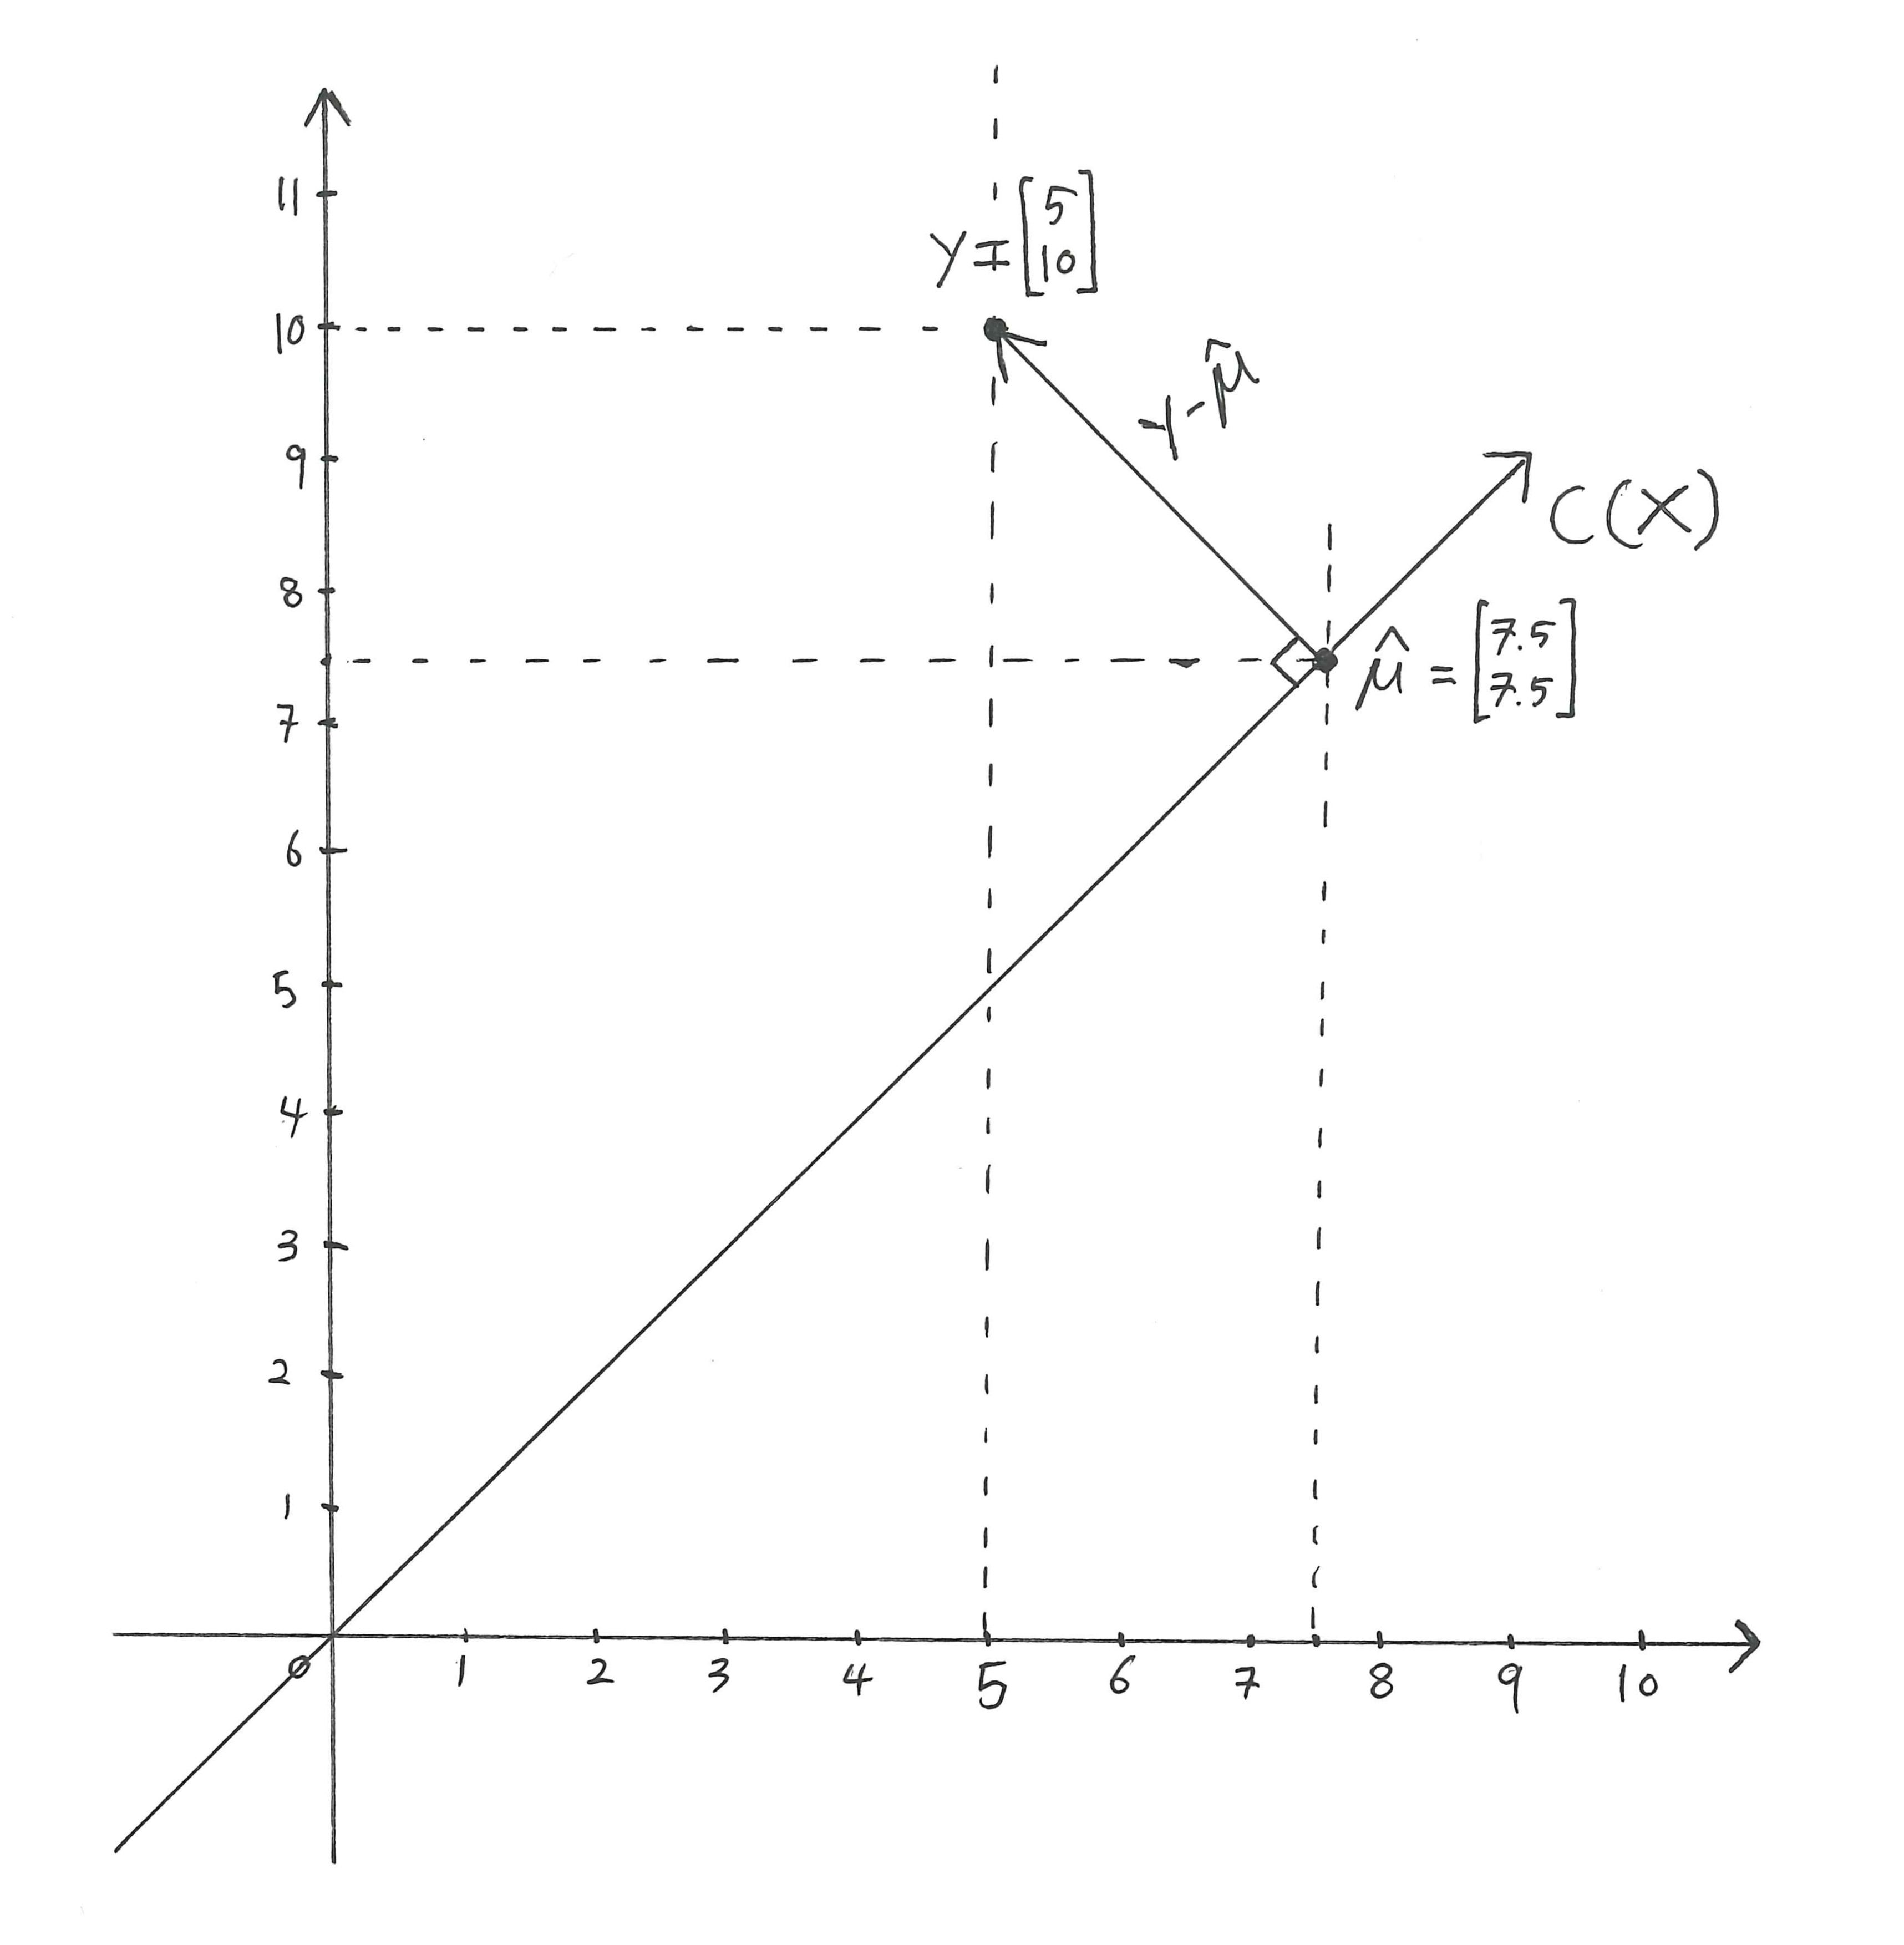
\includegraphics[width=0.7\textwidth]{Exercise_2_22_b.jpeg}
\caption{Visualization of $\bm{y}, \widehat{\bm{\mu}}, C(\bm{X})$}
\end{figure}



\vspace{\baselineskip}
\section{Exercise 2.23}
Consider the saturated model $\E[Y_{i}] = \beta_{i}$, $i = 1, \cdots ,n$.
\subsection{(a)}
\begin{align*}
\bm{X}= \bm{I}_{n}
, \quad
C(\bm{X}) = \left\{\bm{\eta} = \bm{X}\bm{\beta} = \bm{\beta} = 
\begin{bmatrix}
\beta_{1}\\
\vdots\\
\beta_{n}
\end{bmatrix}
\left. \right\vert \bm{\beta} \in \mathbb{R}^{n}
\right\}
= \mathbb{R}^{n}
\end{align*}
Its orthogonal complement is
$C(\bm{X})^{\perp} = \left\{\bm{\tau} = \bm{0}_{n}\right\}$ because we have $\bm{\eta}^{\rm T}\bm{\tau} = 0$.\\
\begin{align*}
\bm{P}_{X} &= \bm{X}(\bm{X}^{\rm T}\bm{X})^{-1}\bm{X}^{\rm T}
= \bm{I}_{n}\\
\bm{I} - \bm{P}_{X} &= \bm{0}_{n \times n}
\end{align*}

\subsection{(b)}
\begin{align*}
\widehat{\bm{\beta}} = \bm{y}, \quad \widehat{\bm{\mu}} = \widehat{\bm{\beta}} = \bm{y}
\end{align*}

\begin{align*}
s = \sqrt{\frac{\sum_{i=1}^{n} (y_{i} - y_{i})^{2}}{n-n}} = \frac{0}{0}
\end{align*}

This saturated model is not sensible for practical use because it's not processing anything. It merely returns the raw information from data as output, namely $\widehat{\mu}_{i} = y_{i}$.


\vspace{\baselineskip}
\section{Exercise 3.2}
Note that we solve this exercise for more general case where $T$ has noncentral $t$-distribution.\\

It's given that $T \sim t_{p,\mu}$. We can rewrite $T$ as
\begin{align*}
T = \frac{Z}{\sqrt{X/p}}
\end{align*}
where $Z \sim N(\mu, 1)$, $X \sim \chi_{p}^2$ and $Z \independent X$. (The notation $A \independent B$ means that $A$ and $B$ are independent.)\\
Let $W = Z^2$, then $W \sim \chi_{1, \mu^2}^2$ (noncentral chi-squared distribution).\\

Now we look at $T^2$:
\begin{align*}
T^2 = \frac{Z^2}{X/p} = \frac{W/1}{X/p}
\end{align*}
where $W \sim \chi_{1, \mu^2}$, $X \sim \chi_{p}^2$ and $W \independent X$.

Then, by definition, $T^2 \sim F_{1,p,\mu^2}$ (noncentral $F$-distribution).

If we let $\mu = 0$, then we have the (central) $F$-distribution.

\vspace{\baselineskip}
\vspace{\baselineskip}
\begin{framed}
The relationship between noncentral $t$-distribution and noncentral $F$-distribution:
\begin{align*}
T \sim t_{p, \mu} ~ \Rightarrow ~ F = T^2 \sim F_{1,p,\mu^2}
\end{align*}
\end{framed}



\vspace{\baselineskip}
\section{Exercise 3.4}
Sum-of-squares decomposition (p.42 of the book): $\bm{Y}^{\rm T}\bm{Y} = \bm{Y}^{\rm T}\bm{P}_{X}\bm{Y} + \bm{Y}^{\rm T}\left(\bm{I} - \bm{P}_{X} \right)\bm{Y}$.

Since $\bm{P}_{X} + (\bm{I} -\bm{P}_{X}) = \bm{I}$, $\bm{Y}^{\rm T}\bm{P}_{X}\bm{Y} \independent \bm{Y}^{\rm T}\left(\bm{I} - \bm{P}_{X}\right)\bm{Y}$ by Cochran's theorem.

In case of null model, $\bm{P}_{X} = \frac{1}{n}\bm{1}_{n}\bm{1}_{n}^{\rm T}$ and we have
\begin{align*}
\bm{Y}^{\rm T}\bm{P}_{X}\bm{Y} &= \bm{Y}^{\rm T}\overline{Y}\bm{1}_{n} = \overline{Y}\bm{Y}^{\rm T}\bm{1}_{n} = n\overline{Y}^2\\
\bm{Y}^{\rm T}\left(\bm{I} - \bm{P}_{X}\right)\bm{Y} &= \bm{Y}^{\rm T}\left(\bm{I} - \bm{P}_{X}\right)^{\rm T}\left(\bm{I} - \bm{P}_{X}\right)\bm{Y} = \left(\bm{Y} - \overline{Y}\bm{1}_{n}\right)^{\rm T}\left(\bm{Y} - \overline{Y}\bm{1}_{n}\right) = \sum_{i=1}^{n} (Y_{i} - \overline{Y})^{2}
\end{align*}
So, $n\overline{Y}^2 \independent \sum_{i=1}^{n} (Y_{i} - \overline{Y})^{2}$ which implies  $\overline{Y}^2 \independent \frac{\sum_{i=1}^{n} (Y_{i} - \overline{Y})^{2}}{n-1} = S^2$.


\vspace{\baselineskip}
\section{Exercise 3.5}
We apply the sum-of-squares decomposition to $(\bm{Y} - \bm{\mu}_{0})$ where $\bm{Y} \sim N(\bm{\mu}, \sigma^2 \bm{I})$, $\bm{\mu_{0}} = \mu_{0}\bm{1}_{n}$, $\bm{\mu} = \mu\bm{1}_{n}$:
\begin{align*}
(\bm{Y} - \bm{\mu}_{0})^{\rm T}(\bm{Y} - \bm{\mu}_{0}) = (\bm{Y} - \bm{\mu}_{0})^{\rm T}\bm{P}_{X}(\bm{Y} - \bm{\mu}_{0}) + (\bm{Y} - \bm{\mu}_{0})^{\rm T}\left(\bm{I} - \bm{P}_{X} \right)(\bm{Y} - \bm{\mu}_{0}).
\end{align*}

Since $\bm{P}_{X} + (\bm{I} -\bm{P}_{X}) = \bm{I}$, Cochran's theorem gives $(\bm{Y} - \bm{\mu}_{0})^{\rm T}\bm{P}_{X}(\bm{Y} - \bm{\mu}_{0}) \independent (\bm{Y} - \bm{\mu}_{0})^{\rm T}\left(\bm{I} - \bm{P}_{X} \right)(\bm{Y} - \bm{\mu}_{0})$ and
\begin{align*}
\frac{(\bm{Y} - \bm{\mu}_{0})^{\rm T}\bm{P}_{X}(\bm{Y} - \bm{\mu}_{0})}{\sigma^2} \sim \chi_{r_{1}, \lambda_{1}}^2
\end{align*}
\begin{align*}
\frac{(\bm{Y} - \bm{\mu}_{0})^{\rm T}\left(\bm{I} - \bm{P}_{X} \right)(\bm{Y} - \bm{\mu}_{0})}{\sigma^2} \sim \chi_{r_{2}, \lambda_{2}}^2
\end{align*}

where $r_{1} = \mathrm{rank}(\bm{P}_{X})$, $\lambda_{1} = \frac{(\bm{\mu} - \bm{\mu}_{0})^{\rm T} \bm{P}_{X} (\bm{\mu} - \bm{\mu}_{0})}{\sigma^2}$ and $r_{2} = \mathrm{rank}(\bm{I} - \bm{P}_{X})$, $\lambda_{2} = \frac{(\bm{\mu} - \bm{\mu}_{0})^{\rm T}\left(\bm{I} - \bm{P}_{X} \right)(\bm{\mu} - \bm{\mu}_{0})}{\sigma^2}$.


In case of null model, $\bm{P}_{X} = \frac{1}{n}\bm{1}_{n}\bm{1}_{n}^{\rm T}$ and we have $\bm{P}_{X}\bm{Y} = \frac{1}{n}\bm{1}_{n}\bm{1}_{n}^{\rm T}\bm{Y} = \overline{Y}\bm{1}_{n}$, $\bm{P}_{X}\bm{\mu} = \frac{1}{n}\bm{1}_{n}\bm{1}_{n}^{\rm T}\bm{1}_{n}\mu = \mu\bm{1}_{n} = \bm{\mu}$.\\

Further,
\begin{align*}
(\bm{Y} - \bm{\mu}_{0})^{\rm T}\bm{P}_{X}(\bm{Y} - \bm{\mu}_{0}) &= (\bm{Y} - \bm{\mu}_{0})^{\rm T}\bm{P}_{X}^{\rm T}\bm{P}_{X}(\bm{Y} - \bm{\mu}_{0})\\
&= (\overline{Y}\bm{1}_{n} - \mu_{0}\bm{1}_{n})^{\rm T}(\overline{Y}\bm{1}_{n} - \mu_{0}\bm{1}_{n}) = (\overline{Y} - \mu_{0})^2 \bm{1}_{n}^{\rm T}\bm{1}_{n}\\
&= n(\overline{Y} - \mu_{0})^2\\
(\bm{Y} - \bm{\mu}_{0})^{\rm T}\left(\bm{I} - \bm{P}_{X} \right)(\bm{Y} - \bm{\mu}_{0}) &= (\bm{Y} - \bm{\mu}_{0})^{\rm T}\left(\bm{I} - \bm{P}_{X} \right)^{\rm T}\left(\bm{I} - \bm{P}_{X} \right)(\bm{Y} - \bm{\mu}_{0})\\
&= (\bm{Y} - \overline{Y}\bm{1}_{n})^{\rm T}(\bm{Y} - \overline{Y}\bm{1}_{n})\\
&= \sum_{i=1}^{n} (Y_{i} - \overline{Y})^{2}
\end{align*}
and
\begin{align*}
r_{1} &= \mathrm{rank}(\bm{P}_{X}) = \mathrm{rank}(\frac{1}{n}\bm{1}_{n}\bm{1}_{n}^{\rm T}) = 1\\
r_{2} &= \mathrm{rank}(\bm{I} - \bm{P}_{X}) = n - 1\\
\lambda_{1} &= \frac{(\bm{\mu} - \bm{\mu}_{0})^{\rm T} \bm{P}_{X} (\bm{\mu} - \bm{\mu}_{0})}{\sigma^2} = \frac{n(\mu - \mu_{0})^2}{\sigma^2}\\
\lambda_{2} &= \frac{(\bm{\mu} - \bm{\mu}_{0})^{\rm T}\left(\bm{I} - \bm{P}_{X} \right)(\bm{\mu} - \bm{\mu}_{0})}{\sigma^2} = \frac{\sum_{i=1}^{n} (\mu - \mu)^{2}}{\sigma^2} = 0.
\end{align*}


So, we have 
\begin{align*}
\frac{n(\overline{Y} - \mu_{0})^2}{\sigma^2} \sim \chi_{1, \lambda_{1}}^2 ~~\mbox{and}~~ \frac{(n-1)S^2}{\sigma^2} = \frac{\sum_{i=1}^{n} (Y_{i} - \overline{Y})^{2}}{\sigma^2} \sim \chi_{n-1}^2
\end{align*}
and they are independent.\\

Then, by the definition of noncentral $F$-distribution,
\begin{align*}
F = \frac{n(\overline{Y} - \mu_{0})^2}{S^2} = \frac{n(\overline{Y} - \mu_{0})^2 / 1}{\sum_{i=1}^{n} (Y_{i} - \overline{Y})^{2} / (n-1)} \sim F_{1, n-1, \lambda_{1}}.
\end{align*}
$F$ is our test statistic.

Null hypothesis $H_{0}: \mu = \mu_{0}$. Under this $H_{0}$, $\lambda_{1} = \frac{n(\mu_{0} - \mu_{0})^2}{\sigma^2} = 0$. So, our test statistic follows (central) $F$-distribution: $F \sim F_{1, n-1}$.

A level $\alpha$ $F$-test rejects the null hypothesis if  $F > f_{1-\alpha, 1, n-1}$.\\
\vspace{\baselineskip}


Now, we construct a $t$-test.\\
Since $Y_{i}, \cdots Y_{n} \stackrel{i.i.d.}{\sim} N(\mu, \sigma^2)$, $\overline{Y} \sim N\left(\mu, \frac{\sigma^2}{n} \right)$ and by transformation $\frac{\sqrt{n}(\overline{Y} -\mu_{0})}{\sigma} \sim N\left(\frac{\sqrt{n}(\mu -\mu_{0})}{\sigma}, 1\right)$.

It's well known that $\frac{(n-1)S^2}{\sigma^2} \sim \chi_{n-1}^2$. (You can easily show this by using the result from p.82 of the book.) By combining those results, we have
\begin{align*}
T = \frac{\frac{\sqrt{n}(\overline{Y} -\mu_{0})}{\sigma}}{\sqrt{\frac{(n-1)S^2}{\sigma^2}/(n-1)}} = \frac{\sqrt{n}(\overline{Y} - \mu_{0})}{S}  \sim t_{n-1, \sqrt{\lambda_{1}}}.
\end{align*}

Under $H_{0}: \mu = \mu_{0}$, $\lambda_{1} = \frac{n(\mu_{0} - \mu_{0})^2}{\sigma^2} = 0$. So, our test statistic follows (central) $t$-distribution: $T \sim t_{n-1}$.

A level $\alpha$ two-sided $t$-test rejects the null hypothesis if  $|T| > t_{1-\frac{\alpha}{2}, n-1}$.

\vspace{\baselineskip}
\section{Exercise 3.7}

\subsection{(a)}
In one-way ANOVA, the following sum of squares decomposition is used:
\begin{align*}
\bm{Y}^{\rm T}\bm{Y} = \bm{Y}^{\rm T}\bm{P}_{0}\bm{Y} +\bm{Y}^{\rm T}\left(\bm{P}_{X} -\bm{P}_{0} \right)\bm{Y} +\bm{Y}^{\rm T}\left(\bm{I} -\bm{P}_{X}\right)\bm{Y}.
\end{align*}
(See p.46 of the book for details.)

The between-groups sum of squares is
\begin{align*}
\bm{Y}^{\rm T}\left(\bm{P}_{X} -\bm{P}_{0} \right)\bm{Y} = \sum_{i=1}^{c} n_{i}\left(\overline{Y}_{i} - \overline{Y}\right)^2.
\end{align*}
By Cochran's theorem, $\frac{\bm{Y}^{\rm T}\left(\bm{P}_{X} -\bm{P}_{0} \right)\bm{Y}}{\sigma^2} \sim \chi_{r, \lambda}^2$ with $r = \mathrm{rank}(\bm{P}_{X} -\bm{P}_{0}) = c-1, \lambda = \frac{\bm{\mu}^{\rm T}\left(\bm{P}_{X} -\bm{P}_{0} \right)\bm{\mu}}{\sigma^2}$.

By replacing $\bm{Y}$ by $\bm{\mu}$ in the expression of between-groups sum of squares, we directly obtain
\begin{align*}
\lambda = \frac{\bm{\mu}^{\rm T}\left(\bm{P}_{X} -\bm{P}_{0} \right)\bm{\mu}}{\sigma^2} = \frac{1}{\sigma^2} \sum_{i=1}^{c} n_{i}\left(\mu_{i} - \overline{\mu}\right)^2
\end{align*}
where $\overline{\mu} = \frac{1}{n} \sum_{i=1}^{c} n_{i} \mu_{i}$.

\subsection{(b)}
To perform $F$-test, we need to evaluate $\bm{Y}^{\rm T}\left(\bm{I} -\bm{P}_{X}\right)\bm{Y}$:
\begin{align*}
\bm{Y}^{\rm T}\left(\bm{I} -\bm{P}_{X}\right)\bm{Y} = \sum_{i=1}^{c} \sum_{j=1}^{n_{i}} \left(Y_{i,j} - \overline{Y}_{i} \right)^2.
\end{align*}


By Cochran's theorem, $\frac{\bm{Y}^{\rm T}\left(\bm{I} -\bm{P}_{X}\right)\bm{Y}}{\sigma^2} \sim \chi_{r_{*} , \lambda_{*}}^2$ where $r_{*} = \mathrm{rank}(\bm{I} -\bm{P}_{X}) = n-c, \lambda_{*} = \frac{\bm{\mu}^{\rm T}\left(\bm{I} -\bm{P}_{X} \right)\bm{\mu}}{\sigma^2} = \frac{1}{\sigma^2} \sum_{i=1}^{c} n_{i}\left(\mu_{i} - \mu_{i}\right)^2 = 0$.


By the definition of noncentral $F$-distribution, we have the test statistic
\begin{align*}
F = \frac{\frac{\sum_{i=1}^{c} n_{i}\left(\overline{Y}_{i} - \overline{Y}\right)^2}{\sigma^2}/(c-1)}{\frac{\sum_{i=1}^{c} \sum_{j=1}^{n_{i}} \left(Y_{i,j} - \overline{Y}_{i} \right)^2}{\sigma^2} / (n-c)} \sim \frac{\chi_{c-1, \lambda}^2 / (c-1)}{\chi_{n-c}^2 / (n-c)} = F_{c-1,n-c,\lambda}
\end{align*}

Now, we evaluate the noncentrality parameter $\lambda$ by using given conditions:
\begin{align*}
\lambda &= \frac{1}{\sigma^2} \sum_{i=1}^{c} n_{i}\left(\mu_{i} - \overline{\mu}\right)^2\\
&= \frac{n}{\sigma^2}\left[\left(\mu_{1} - \overline{\mu}\right)^2 + \left(\mu_{2} - \overline{\mu}\right)^2 + \left(\mu_{3} - \overline{\mu}\right)^2 \right]\\
&= \frac{n}{9\sigma^2}\left[\left(3\mu_{1} - (\mu_{1} + \mu_{2} + \mu_{3})\right)^2 + \left(3\mu_{2} - (\mu_{1} + \mu_{2} + \mu_{3})\right)^2 + \left(3\mu_{3} - (\mu_{1} + \mu_{2} + \mu_{3})\right)^2 \right]\\
&= \frac{n}{9\sigma^2}\left[\left( (\mu_{1} - \mu_{2}) + (\mu_{1} - \mu_{3}) \right)^2 + \left( -(\mu_{1} - \mu_{2}) + (\mu_{2} - \mu_{3}) \right)^2 + \left( -(\mu_{1} - \mu_{3}) - (\mu_{2} - \mu_{3}) \right)^2 \right]\\
&= \frac{n}{9\sigma^2}\left[\left( (\mu_{1} - \mu_{2}) + (\mu_{1} - \mu_{3}) \right)^2 + \left( -(\mu_{1} - \mu_{2}) + (\mu_{2} - \mu_{3}) \right)^2 + \left( -(\mu_{1} - \mu_{3}) - (\mu_{2} - \mu_{3}) \right)^2 \right]\\
&= \frac{n}{9\sigma^2}\left[\left(\frac{\sigma}{2} + \sigma \right)^2 + \left(-\frac{\sigma}{2} + \frac{\sigma}{2} \right)^2 + \left(-\sigma -\frac{\sigma}{2} \right)^2  \right]\\
&= \frac{n}{9\sigma^2}\left(\frac{9\sigma^2}{2} \right)\\
&= \frac{n}{2}.
\end{align*}


So, our test statistic becomes
\begin{align*}
F_{2,n-3,\frac{n}{2}}
\end{align*}
and level $0.05$ $F$-test rejects the null hypothesis if  $F > f_{0.95, 2, n-3}$.\\

Now, we calculate power.
\begin{align*}
\mbox{Power} &= \Pr\left(\mbox{reject}~H_{0}|H_{1}~\mbox{is true}\right)\\
&= \Pr\left(F_{2,n-3,\frac{n}{2}} > f_{0.95, 2, n-3}\right)\\
&= 1 - \Pr\left(F_{2,n-3,\frac{n}{2}} \leq f_{0.95, 2, n-3}\right)\\
&= 1 - G\left(f_{0.95, 2, n-3}\right)
\end{align*}

Calculation in \texttt{R}:
\begin{lstlisting}
> alpha = 0.05
> c.val = 3
> n = c(10, 30, 50)
> lambda = n/2
> 
> df.1 = c.val - 1
> df.2 = c.val*n - c.val
> 
> critic.val = qf(1 - alpha, df.1 , df.2) # 0.95 quantile of F dist
> power.val = 1 - pf(critic.val, df.1, df.2, lambda) # right-tail prob. for noncentral F
> 
> result.mat = data.frame(n = n, critic.val = critic.val, power.val = power.val)
> show(result.mat)
   n critic.val power.val
1 10   3.354131 0.4579923
2 30   3.101296 0.9362768
3 50   3.057621 0.9959038
\end{lstlisting}


\subsection{(c)}
\begin{align*}
\lambda &= \frac{1}{\sigma^2} \sum_{i=1}^{c} n_{i}\left(\mu_{i} - \overline{\mu}\right)^2\\
&= \frac{n}{\sigma^2}\left[\left(\mu_{1} - \overline{\mu}\right)^2 + \left(\mu_{2} - \overline{\mu}\right)^2 + \left(\mu_{3} - \overline{\mu}\right)^2 \right]\\
&= \frac{n}{9\sigma^2}\left[\left(3\mu_{1} - (\mu_{1} + \mu_{2} + \mu_{3})\right)^2 + \left(3\mu_{2} - (\mu_{1} + \mu_{2} + \mu_{3})\right)^2 + \left(3\mu_{3} - (\mu_{1} + \mu_{2} + \mu_{3})\right)^2 \right]\\
&= \frac{n}{9\sigma^2}\left[\left( (\mu_{1} - \mu_{2}) + (\mu_{1} - \mu_{3}) \right)^2 + \left( -(\mu_{1} - \mu_{2}) + (\mu_{2} - \mu_{3}) \right)^2 + \left( -(\mu_{1} - \mu_{3}) - (\mu_{2} - \mu_{3}) \right)^2 \right]\\
&= \frac{n}{9\sigma^2}\left[\left( (\mu_{1} - \mu_{2}) + (\mu_{1} - \mu_{3}) \right)^2 + \left( -(\mu_{1} - \mu_{2}) + (\mu_{2} - \mu_{3}) \right)^2 + \left( -(\mu_{1} - \mu_{3}) - (\mu_{2} - \mu_{3}) \right)^2 \right]\\
&= \frac{n}{9\sigma^2}\left[\left(\Delta\sigma + 2\Delta\sigma \right)^2 + \left(-\Delta\sigma + \Delta\sigma \right)^2 + \left(-2\Delta\sigma -\Delta\sigma \right)^2 \right]\\
&= \frac{n}{9\sigma^2} \cdot 2(3\Delta\sigma)^2\\
&= 2n\Delta^2
\end{align*}

Calculation in \texttt{R}:
\begin{lstlisting}
> alpha = 0.05
> c.val = 3
> n = 10
> Delta = c(0, 0.5, 1)
> lambda = 2*n*Delta^2
> 
> df.1 = c.val - 1
> df.2 = c.val*n - c.val
> 
> critic.val = qf(1 - alpha, df.1 , df.2) # 0.95 quantile of F dist
> power.val = 1 - pf(critic.val, df.1, df.2, lambda) # right-tail prob. for noncentral F
> 
> result.mat = data.frame(Delta = Delta, critic.val = critic.val, power.val = power.val)
> show(result.mat)
  Delta critic.val power.val
1   0.0   3.354131 0.0500000
2   0.5   3.354131 0.4579923
3   1.0   3.354131 0.9732551
\end{lstlisting}


\vspace{\baselineskip}
\section{Exercise 3.9}


\subsection{(a)}
\begin{align*}
\E[\bm{Y}] = \bm{X}\bm{\beta}
\end{align*}
where
\begin{align*}
\bm{Y} =
\begin{bmatrix}
\bm{Y}_{1}\\
\bm{Y}_{2}
\end{bmatrix}
, \quad
\bm{X} = 
\begin{bmatrix}
\bm{1}_{n_{1}} & \bm{1}_{n_{1}}\\
\bm{1}_{n_{2}} & \bm{0}_{n_{2}}
\end{bmatrix}
, \quad
\bm{\beta} =
\begin{bmatrix}
\beta_{0}\\
\beta_{1}
\end{bmatrix}
\end{align*}

Interpretation:\\
Note that $\mu_{1} = \beta_{0} + \beta_{1}$ and $\mu_{2} = \beta_{0}$. Therefore, $\beta_{0} = \mu_{2}$ and $\beta_{1} = \mu_{1} - \mu_{2}$.


\subsection{(b)}
Use equation (2.6) from p.45 of the book.
\begin{align*}
\bm{P}_{X} = 
\begin{bmatrix}
\frac{1}{n_{1}}\bm{1}_{n_{1}}\bm{1}_{n_{1}}^{\rm T} & \bm{0}\\
\bm{0} & \frac{1}{n_{2}}\bm{1}_{n_{2}}\bm{1}_{n_{2}}^{\rm T}
\end{bmatrix}
\end{align*}

Realize that this exercise is a special case of exercise 3.7 with $c = 2$. We simply use the results from exercise 3.7.
\begin{align*}
\mathrm{SSE} &= \sum_{i=1}^{2} \sum_{j=1}^{n_{i}} \left(Y_{i,j} - \overline{Y}_{i} \right)^2 = \bm{Y}^{\rm T}\left(\bm{I} -\bm{P}_{X}\right)\bm{Y}\\
\mathrm{SSR} &= \sum_{i=1}^{2} n_{i}\left(\overline{Y}_{i} - \overline{Y}\right)^2 = \bm{Y}^{\rm T}\left(\bm{P}_{X} -\bm{P}_{0} \right)\bm{Y}
\end{align*}
(For definitions of SSR and SSE, see p.51 of the book.)


\subsection{(c)}
In exercise 3.7, we showed:
\begin{align*}
F &= \frac{\frac{\bm{Y}^{\rm T}\left(\bm{P}_{X} -\bm{P}_{0} \right)\bm{Y}}{\sigma^2}/(c-1)}{\frac{\bm{Y}^{\rm T}\left(\bm{I} -\bm{P}_{X}\right)\bm{Y}}{\sigma^2}/(n-c)}\\
&= \frac{\frac{\sum_{i=1}^{c} n_{i}\left(\overline{Y}_{i} - \overline{Y}\right)^2}{\sigma^2}/(c-1)}{\frac{\sum_{i=1}^{c} \sum_{j=1}^{n_{i}} \left(Y_{i,j} - \overline{Y}_{i} \right)^2}{\sigma^2}/(n-c)}\\
&\sim \frac{\chi_{c-1, \lambda}^2 / (c-1)}{\chi_{n-c}^2 / (n-c)}\\
&= F_{c-1,n-c,\lambda}
\end{align*}
where
\begin{align*}
\lambda = \frac{\bm{\mu}^{\rm T}\left(\bm{P}_{X} -\bm{P}_{0} \right)\bm{\mu}}{\sigma^2} = \frac{1}{\sigma^2} \sum_{i=1}^{c} n_{i}\left(\mu_{i} - \overline{\mu}\right)^2.
\end{align*}

In our case with $c = 2$, it becomes
\begin{align*}
F &= \frac{\frac{\sum_{i=1}^{2} n_{i}\left(\overline{Y}_{i} - \overline{Y}\right)^2}{\sigma^2}}{\frac{\sum_{i=1}^{2} \sum_{j=1}^{n_{i}} \left(Y_{i,j} - \overline{Y}_{i} \right)^2}{\sigma^2}/(n_{1}+n_{2}-2)}\\
&\sim \frac{\chi_{1, \lambda}^2}{\chi_{n-2}^2 / (n_{1}+n_{2}-2)}\\
&= F_{1,n-2,\lambda}
\end{align*}
where
\begin{align*}
\lambda = \frac{\bm{\mu}^{\rm T}\left(\bm{P}_{X} -\bm{P}_{0} \right)\bm{\mu}}{\sigma^2} = \frac{1}{\sigma^2} \sum_{i=1}^{2} n_{i}\left(\mu_{i} - \overline{\mu}\right)^2.
\end{align*}

Notice that
\begin{align*}
\sum_{i=1}^{2} n_{i}\left(\overline{Y}_{i} - \overline{Y}\right)^2
&= n_{1}\left(\overline{Y}_{1} - \overline{Y}\right)^2 + n_{2}\left(\overline{Y}_{2} - \overline{Y}\right)^2\\
&= n_{1}\left(\frac{n_{1}\overline{Y}_{1}+n_{2}\overline{Y}_{1}-n_{1}\overline{Y}_{1}-n_{2}\overline{Y}_{2}}{n_{1}+n_{2}}\right)^2 + n_{2}\left(\frac{n_{1}\overline{Y}_{2}+n_{2}\overline{Y}_{2}-n_{1}\overline{Y}_{1}-n_{2}\overline{Y}_{2}}{n_{1}+n_{2}}\right)^2\\
&= n_{1}\left(\frac{n_{2}\overline{Y}_{1}-n_{2}\overline{Y}_{2}}{n_{1}+n_{2}}\right)^2 + n_{2}\left(\frac{n_{1}\overline{Y}_{2}-n_{1}\overline{Y}_{1}}{n_{1}+n_{2}}\right)^2\\
&= \frac{(\overline{Y}_{1} - \overline{Y}_{2})^2}{(n_{1}+n_{2})^2} n_{1}n_{2}^2 + \frac{(\overline{Y}_{1} - \overline{Y}_{2})^2}{(n_{1}+n_{2})^2} n_{1}^2 n_{2}\\
&= (\overline{Y}_{1} - \overline{Y}_{2})^2 \frac{n_{1}n_{2}(n_{1}+n_{2})}{(n_{1}+n_{2})^2}\\
&= (\overline{Y}_{1} - \overline{Y}_{2})^2 \frac{n_{1}n_{2}}{n_{1}+n_{2}}\\
&= (\overline{Y}_{1} - \overline{Y}_{2})^2 \left(\frac{n_{1}+n_{2}}{n_{1}n_{2}}\right)^{-1}\\
&= (\overline{Y}_{1} - \overline{Y}_{2})^2 \left(\frac{1}{n_{1}} + \frac{1}{n_{2}}\right)^{-1}
\end{align*}
and
\begin{align*}
\frac{1}{n_{1} +n_{2} -2}\sum_{i=1}^{2} \sum_{j=1}^{n_{i}} \left(Y_{i,j} - \overline{Y}_{i} \right)^2
&= \frac{1}{n_{1} +n_{2} -2}\sum_{i=1}^{2} \sum_{j=1}^{n_{i}} (n_{i}-1)\frac{\left(Y_{i,j} - \overline{Y}_{i} \right)^2}{n_{i}-1}\\
&= \frac{1}{n_{1} +n_{2} -2}\sum_{i=1}^{2} (n_{i}-1) S_{i}^2\\
&= \frac{n_{1} - 1}{n_{1} +n_{2} -2} S_{1}^2 + \frac{n_{2} - 1}{n_{1} +n_{2} -2} S_{2}^2\\
&= S^2.
\end{align*}
(This famous result has the name \textit{pooled variance}.)

Thus,
\begin{align*}
F &= \frac{\frac{\sum_{i=1}^{2} n_{i}\left(\overline{Y}_{i} - \overline{Y}\right)^2}{\sigma^2}}{\frac{\sum_{i=1}^{2} \sum_{j=1}^{n_{i}} \left(Y_{i,j} - \overline{Y}_{i} \right)^2}{\sigma^2}/(n_{1}+n_{2}-2)}\\
&= \frac{(\overline{Y}_{1} - \overline{Y}_{2})^2 \left(\frac{1}{n_{1}} + \frac{1}{n_{2}}\right)^{-1}}{S^2}\\
&= \frac{(\overline{Y}_{1} - \overline{Y}_{2})^2}{S^2\left(\frac{1}{n_{1}} + \frac{1}{n_{2}}\right)}\\
&\sim \frac{\chi_{1, \lambda}^2}{\chi_{n_{1}+n_{2}-2}^2 / (n_{1}+n_{2}-2)}\\
&= F_{1,n_{1}+n_{2}-2,\lambda}
\end{align*}

Null hypothesis $H_{0}: \mu_{1} = \mu_{2}$. Under this $H_{0}$, $\lambda = 0$.
So, the null distribution is $F_{1,n-2}$


\subsection{(d)}
Notice that $\overline{Y}_{1} - \overline{Y}_{2} \sim N\left(\mu_{1} - \mu_{2}, \frac{\sigma^2}{n_{1}} + \frac{\sigma^2}{n_{2}}\right)$, which can be transformed into $\frac{\overline{Y}_{1} - \overline{Y}_{2}}{\sigma\sqrt{\frac{1}{n_{1}} + \frac{1}{n_{2}}}} \sim N\left(\frac{\mu_{1} - \mu_{2}}{\sigma\sqrt{\frac{1}{n_{1}} + \frac{1}{n_{2}}}}, 1\right)$.\\
Further, $\frac{(n_{1} +n_{2} -2)S^2}{\sigma^2} \sim \chi_{n_{1} +n_{2} -2}^2$.\\

So, 
\begin{align*}
T = \frac{\frac{\overline{Y}_{1} - \overline{Y}_{2}}{\sigma\sqrt{\frac{1}{n_{1}} + \frac{1}{n_{2}}}}}{\sqrt{\frac{(n_{1} +n_{2} -2)S^2}{\sigma^2}/(n_{1} +n_{2} -2)}} = \frac{\overline{Y}_{1} - \overline{Y}_{2}}{S\sqrt{\frac{1}{n_{1}} + \frac{1}{n_{2}}}} \sim t_{n_{1} +n_{2} -2, \lambda}
\end{align*}
where $\lambda = \frac{\mu_{1} - \mu_{2}}{\sigma\sqrt{\frac{1}{n_{1}} + \frac{1}{n_{2}}}}$.\\
Under $H_{0}: \mu_{1} = \mu_{2}$, $\lambda = 0$ and $T \sim t_{n_{1} +n_{2} -2}$.


\vspace{\baselineskip}
\section{Exercise 3.17}
\subsection{(a)}
p.93 of the book gives description of \textit{general linear hypothesis} including corresponding $F$-test statistic.\\
In our case, we impose 1 constraint ($\beta_{j} = \beta_{k}$) to the model with $n$ observations and $p$ parameters.

For normal linear model, it's well known that
\begin{align*}
\widehat{\bm{\beta}} \sim N\left(\bm{\beta}, \sigma^2 (\bm{X}^{\rm T}\bm{X})^{-1} \right).
\end{align*}
By multiplying $\bm{\beta}$ with a row vector $\bm{\Lambda}$, we obtain
\begin{align*}
\bm{\Lambda}\widehat{\bm{\beta}} \sim N\left(\bm{\Lambda}\bm{\beta}, \sigma^2 \bm{\Lambda}(\bm{X}^{\rm T}\bm{X})^{-1}\bm{\Lambda}^{\rm T} \right).
\end{align*}
By using the result from p.82 of the book, we have
\begin{align*}
\left(\bm{\Lambda}{\widehat{\bm{\beta}}} - \bm{\Lambda}\bm{\beta}\right)^{\rm T}\left[\sigma^2\bm{\Lambda} (\bm{X}^{\rm T}\bm{X})^{-1} \bm{\Lambda}^{\rm T} \right]^{-1}\left(\bm{\Lambda}{\widehat{\bm{\beta}}} - \bm{\Lambda}\bm{\beta}\right) \sim \chi_{p}^2
\end{align*}
where $p = \mathrm{rank}(\bm{\Lambda}\bm{\Lambda}^{\rm T})$.\\

We choose $\bm{\Lambda}$ such that $\bm{\Lambda}$ is a $1 \times p$ vector of 0's except 1 in position $j$ and $-1$ in position $k$. Then we have $\bm{\Lambda}\bm{\beta} = \beta_{j} - \beta_{k}$ and the null-hypothesis can be written as: $H_{0}: \bm{\Lambda}\bm{\beta} = \beta_{j} - \beta_{k} = 0$. This gives us
\begin{align*}
\left(\bm{\Lambda}{\widehat{\bm{\beta}}}\right)^{\rm T}\left[\sigma^2\bm{\Lambda} (\bm{X}^{\rm T}\bm{X})^{-1} \bm{\Lambda}^{\rm T} \right]^{-1}\bm{\Lambda}{\widehat{\bm{\beta}}} \sim \chi_{1}^2.
\end{align*}
Note that $\frac{(n-p)S^2}{\sigma^2} \sim \chi_{n-p}^2$.\\

We build our test statistic
\begin{align*}
F &= \frac{(\bm{\Lambda}{\widehat{\bm{\beta}}})^{\rm T}\left[\sigma^2\bm{\Lambda} (\bm{X}^{\rm T}\bm{X})^{-1} \bm{\Lambda}^{\rm T} \right]^{-1}\bm{\Lambda}{\widehat{\bm{\beta}}}/1}{\frac{(n-p)S^2}{\sigma^2}/(n-p)}\\
&= \frac{(\bm{\Lambda}{\widehat{\bm{\beta}}})^{\rm T}\left[\bm{\Lambda} (\bm{X}^{\rm T}\bm{X})^{-1} \bm{\Lambda}^{\rm T} \right]^{-1}\bm{\Lambda}{\widehat{\bm{\beta}}}}{S^2}\\
&= \frac{(\bm{\Lambda}{\widehat{\bm{\beta}}})^{\rm T}\bm{\Lambda}{\widehat{\bm{\beta}}}}{S^2 \bm{\Lambda} (\bm{X}^{\rm T}\bm{X})^{-1} \bm{\Lambda}^{\rm T}}\\
&= \frac{\left(\beta_{j} - \beta_{k} \right)^2}{S^2 \bm{\Lambda} (\bm{X}^{\rm T}\bm{X})^{-1} \bm{\Lambda}^{\rm T}}\\
&\sim \frac{\chi_{1}^2}{\chi_{n-p}^2}\\
&\sim F_{1,n-p}.
\end{align*}
and perform $F$-test.


\vspace{\baselineskip}
\section{Exercise 4.4}

i)\\
From p.124 of the book, we have $\frac{\partial L(\bm{\beta})}{\partial \beta_{j}} = \sum_{i=1}^{n}\frac{(y_{i}-\mu_{i})x_{i,j}}{\Var(Y_{i})}\frac{\partial \mu_{i}}{\partial \eta_{i}} = 0$. By replacing $x_{i,j}$ with $\frac{\partial \eta_{i}}{\partial \beta_{j}}$, we obtain
\begin{align*}
\frac{\partial L(\bm{\beta})}{\partial \beta_{j}} = \sum_{i=1}^{n}\frac{(y_{i}-\mu_{i})x_{i,j}}{\Var(Y_{i})}\frac{\partial \mu_{i}}{\partial \eta_{i}} = \sum_{i=1}^{n}\frac{(y_{i}-\mu_{i})}{\Var(Y_{i})}\frac{\partial \mu_{i}}{\partial \eta_{i}}\frac{\partial \eta_{i}}{\partial \beta_{j}} = \sum_{i=1}^{n}\frac{(y_{i}-\mu_{i})}{\Var(y_{i})}\frac{\partial \mu_{i}}{\partial \beta_{j}} = 0
\end{align*}

ii)\\
In generalized least squares, $M = \sum_{i=1}^{n}\frac{(y_{i}-\mu_{i})^{2}}{\Var(y_{i})}$ is minimized with respect to model parameters. The solution then should satisfy $\frac{\partial M}{\partial \beta_{j}} = \frac{\partial \sum_{i=1}^{n}\frac{(y_{i}-\mu_{i})^{2}}{\Var(y_{i})}}{\partial \beta_{j}} = 0$ for all $j =  1, \cdots, p$. So,

\begin{align*}
\frac{\partial M}{\partial \beta_{j}} = \sum_{i=1}^{n} \frac{1}{\Var(y_{i})}\frac{\partial (y_{i}-\mu_{i})^{2}}{\partial \mu_{i}}\frac{\partial \mu_{i}}{\partial \beta_{j}} = -2\sum_{i=1}^{n}\frac{(y_{i}-\mu_{i})}{\Var(y_{i})}\frac{\partial \mu_{i}}{\partial \beta_{j}} = 0.
\end{align*}
By simplifying the last part, we obtain $\sum_{i=1}^{n}\frac{(y_{i}-\mu_{i})}{\Var(y_{i})}\frac{\partial \mu_{i}}{\partial \beta_{j}} = 0$.



\vspace{\baselineskip}
\section{Exercise 4.6}
Notice that
\begin{align*}
\Var(Y_{i}) = \mu_{i} =
\begin{cases}
\mu_{A} = g^{-1}(\eta_{A}) = \exp(\eta_{A}) = \exp(\beta_{0} + \beta_{1}) ~~&\mbox{if}~~~ 1 \leq i \leq n_{A}\\
\mu_{B} = g^{-1}(\eta_{B}) = \exp(\eta_{B}) = \exp(\beta_{0}) ~~&\mbox{if}~~~ n_{A}+1 \leq i \leq n_{A}+n_{B}\\
\end{cases}.
\end{align*}
So, we have
\begin{align*}
\frac{\partial L(\bm{\beta})}{\partial \beta_{0}} &= \sum_{i=1}^{n_{A}+n_{B}}\frac{(y_{i}-\mu_{i})\cdot 1}{\Var(Y_{i})}\frac{\partial \mu_{i}}{\partial \eta_{i}}\\
&= \sum_{i=1}^{n_{A}}\frac{(y_{i}-\mu_{i})}{e^{\eta_{A}}}e^{\eta_{A}} + \sum_{i=n_{A}+1}^{n_{B}}\frac{(y_{i}-\mu_{i})}{e^{\eta_{B}}}e^{\eta_{B}}\\
&= \sum_{i=1}^{n_{A}}(y_{i}-\mu_{i}) + \sum_{i=n_{A}+1}^{n_{B}}(y_{i}-\mu_{i})\\
&= 0\\ \intertext{and}
\frac{\partial L(\bm{\beta})}{\partial \beta_{1}} &= \sum_{i=1}^{n}\frac{(y_{i}-\mu_{i})x_{i}}{\Var(Y_{i})}\frac{\partial \mu_{i}}{\partial \eta_{i}}\\
&= \sum_{i=1}^{n_{A}}\frac{(y_{i}-\mu_{i})\cdot 1}{\Var(Y_{i})}\frac{\partial \mu_{i}}{\partial \eta_{i}}\\
&= \sum_{i=1}^{n_{A}}\frac{(y_{i}-\mu_{i})}{e^{\eta_{A}}}e^{\eta_{A}}\\
&= \sum_{i=1}^{n_{A}}(y_{i}-\mu_{i})\\
&= 0.
\end{align*}
This implies $\sum_{i=1}^{n_{A}}(y_{i}-\mu_{i}) = \sum_{i=1}^{n_{A}}(y_{i}-\mu_{A}) = 0$ and $\sum_{i=n_{A}+1}^{n_{B}}(y_{i}-\mu_{i}) = \sum_{i=n_{A}+1}^{n_{B}}(y_{i}-\mu_{B}) = 0$.\\
Thus, $\widehat{\mu}_{A} = \frac{1}{n_{A}}\sum_{i=1}^{n_{A}} y_{i}$ and $\widehat{\mu}_{B} = \frac{1}{n_{B}}\sum_{i=n_{A}+1}^{n_{A}+n_{B}} y_{i}$.



\vspace{\baselineskip}
\section{Exercise 4.9}
From p.126 of the book, we have that $\bm{W}$ is a diagonal matrix with diagonal elements $w_{i} = \frac{1}{\Var(Y_{i})}\left(\frac{\partial \mu_{i}}{\partial \eta_{i}}\right)^{2}$. Under ordinary normal linear model, $g(\mu) = \mu = \eta$. So, $\frac{\partial \mu_{i}}{\partial \eta_{i}} = 1$ and $w_{i} = \frac{1}{\Var(Y_{i})}$. Consequently, $\bm{W} = \sigma^{-2}\bm{I}$.\\
By plugging this result into $\Var(\widehat{\bm{\beta}}) = \left(\bm{X}^{\rm T}\bm{W}\bm{X}\right)^{-1}$, we obtain $\Var(\widehat{\bm{\beta}}) = \sigma^{2}\left(\bm{X}^{\rm T}\bm{X}\right)^{-1}$.


\vspace{\baselineskip}
\section{Exercise 4.12}

% Solution from Ørnulf
We consider a GLM  with linear predictor $\eta_i =\sum_{j=1}^{p} x_{i,j} \beta_{j} =\bm{x}_{i} \bm{\beta}$ and link function $g(\mu_{i})=\eta_{i}$.

We want to find a confidence interval for $\mu=E[Y|\bm{x}_0]$.

It is well known that (cf. page 126 in the book)
\begin{align*}
\widehat{\bm{\beta}} \sim N\left(\bm{\beta}, (\bm{X}^{\rm T}\bm{W}\bm{X})^{-1} \right),\quad \mbox{approximately}
\end{align*}
So,
\begin{align*}
\widehat{\eta} = \bm{x}_{0}\widehat{\bm{\beta}} \sim N\left(\eta = \bm{x}_{0}\bm{\beta}, \, \bm{x}_{0}(\bm{X}^{\rm T}\bm{W}\bm{X})^{-1}\bm{x}_{0}^{\rm T} \right),\quad \mbox{approximately}
\end{align*}
By reformulating this, we have
\begin{align*}
\frac{\widehat{\eta}-\eta}{\sqrt{\bm{x}_{0}(\bm{X}^{\rm T}\bm{W}\bm{X})^{-1}\bm{x}_{0}^{\rm T}}} \sim N(0,1), \quad \mbox{approximately},
\end{align*}

Note that $\widehat{\bm{W}} ~\overset{p}{\to}~ \bm{W}$. Then, it follows from Slutsky's theorem that
\begin{align*}
\frac{\widehat{\eta}-\eta}{\sqrt{\bm{x}_{0}(\bm{X}^{\rm T}\bm{W}\bm{X})^{-1}\bm{x}_{0}^{\rm T}}} &= 
\frac{\widehat{\eta}-\eta}{\sqrt{\bm{x}_{0}(\bm{X}^{\rm T}\widehat{\bm{W}}\bm{X})^{-1}\bm{x}_{0}^{\rm T}}}\cdot\frac{\sqrt{\bm{x}_{0}(\bm{X}^{\rm T}\widehat{\bm{W}}\bm{X})^{-1}\bm{x}_{0}^{\rm T}}}{\sqrt{\bm{x}_{0}(\bm{X}^{\rm T}\bm{W}\bm{X})^{-1}\bm{x}_{0}^{\rm T}}}\\
&\overset{p}{\to}~ \frac{\widehat{\eta}-\eta}{\sqrt{\bm{x}_{0}(\bm{X}^{\rm T}\widehat{\bm{W}}\bm{X})^{-1}\bm{x}_{0}^{\rm T}}} \cdot 1\\
&\sim N(0,1), \quad \mbox{approximately},
\end{align*}
where $\widehat{\bm{W}}$ is $\bm{W}$ evaluated at $\widehat{\bm{\beta}}$. By a standard argument, we obtain an approximate $100(1-\alpha){\%}$ confidence interval for $\eta$ as
\begin{align*}
\left[\, \widehat{\eta} -z_{1-\frac{\alpha}{2}}\sqrt{\bm{x}_{0}(\bm{X}^{\rm T}\widehat{\bm{W}}\bm{X})^{-1}\bm{x}_{0}^{\rm T}}\, , \, \widehat{\eta} +z_{1-\frac{\alpha}{2}}\sqrt{\bm{x}_{0}(\bm{X}^{\rm T}\widehat{\bm{W}}\bm{X})^{-1}\bm{x}_{0}^{\rm T}} \, \right]
\end{align*}
Finally we obtain an approximate $100(1-\alpha){\%}$ confidence interval for $\mu=g^{-1}(\eta)$ by transforming the limits of this confidence interval, i.e.
\begin{align*}
\left[\, g^{-1}\left(\widehat{\eta} -z_{1-\frac{\alpha}{2}}\sqrt{\bm{x}_{0}(\bm{X}^{\rm T}\widehat{\bm{W}}\bm{X})^{-1}\bm{x}_{0}^{\rm T}}\,\right)\, , \, g^{-1}\left(\widehat{\eta} +z_{1-\frac{\alpha}{2}}\sqrt{\bm{x}_{0}(\bm{X}^{\rm T}\widehat{\bm{W}}\bm{X})^{-1}\bm{x}_{0}^{\rm T}}\,\right) \,  \right]
\end{align*}

Note that this ``naive'' method only works when $g^{-1}(\cdot)$ is a monotonic function (at the bottom of p.127 in the book).


%%%%%%%%%%%%%%%%%%%%%%%%
%% Alternative solution with Delta method
%\vspace{\baselineskip}
%\section{Exercise 4.12}
%We obtain the confidence interval of $\mu = \E[Y]$ for a given data point $\bm{x}_{0}$, by transforming the confidence interval for $\eta$ with Delta method.
%
%\vspace{0.5cm}
%\begin{framed}
%\textit{Multivariate Delta method}\\
%
%Suppose that
%\begin{align*}
%\sqrt{n}(\bm{X}_{n} - \bm{\eta}) ~\overset{d}{\to}~ N_{r}\left(\bm{0}, \bm{\Sigma}\right),
%\end{align*}
%for some $r$-dimensional random vector $\bm{X}_{n}$ depending on $n$. If $S$ is a function $\mathbb{R}^{r} \to \mathbb{R}^{s}$ which is once differentiable at $\bm{\eta}$ and has Jacobian matrix $\dot{\bm{S}}(\bm{\eta})$, then
%\begin{align*}
%\sqrt{n}\left(S(\bm{X}_{n}) - S(\bm{\eta})\right) ~\overset{d}{\to}~ N_{s}\left(\bm{0},~ \dot{\bm{S}}(\bm{\eta})^{\rm T} \, \bm{\Sigma} \, \dot{\bm{S}}(\bm{\eta})\right),
%\end{align*}
%provided that $\dot{\bm{S}}(\bm{\eta})^{\rm T} \, \bm{\Sigma} \, \dot{\bm{S}}(\bm{\eta})$ is positive definite.
%\end{framed}
%\vspace{\baselineskip}
%
%For GLM, it's well known that 
%\begin{align*}
%\widehat{\bm{\beta}} \sim N\left(\bm{\beta}, (\bm{X}^{\rm T}\bm{W}\bm{X})^{-1} \right).
%\end{align*}
%So,
%\begin{align*}
%\widehat{\eta} = \bm{x}_{0}\widehat{\bm{\beta}} \sim N\left(\eta = \bm{x}_{0}\bm{\beta}, \, \bm{x}_{0}(\bm{X}^{\rm T}\bm{W}\bm{X})^{-1}\bm{x}_{0}^{\rm T} \right).
%\end{align*}
%By applying Delta method, we obtain
%\begin{align*}
%\widehat{\mu} = g^{-1}(\widehat{\eta}) \sim N\left(g^{-1}\left(\eta\right),~ \dot{S}(\eta)^{\rm T}\bm{x}_{0}(\bm{X}^{\rm T}\bm{W}\bm{X})^{-1}\bm{x}_{0}^{\rm T}\dot{S}(\eta) \right)
%\end{align*}
%where $\dot{S}(\eta) = \frac{\partial g^{-1}(\eta)}{\partial \eta}$ and $\eta = \bm{x}_{0}\bm{\beta}$.\\
%
%By using this results, we obtain
%\begin{align*}
%Z = \frac{\widehat{\mu}-\mu}{\sqrt{\dot{S}(\eta)^{\rm T}\bm{x}_{0}(\bm{X}^{\rm T}\bm{W}\bm{X})^{-1}\bm{x}_{0}^{\rm T}\dot{S}(\eta)}} \sim N(0,1).
%\end{align*}
%
%{\color{red}
%Up to here it's okay to use this Delta method approach. However, we can also just convert the lower and upper bound by using $g^{-1}(\cdot)$ since $g(\cdot)$ is a monotonic function.\\
%
%From here, the approach is wrong because $\frac{(n-p-1)\widehat{\sigma}^2}{\sigma^2} \sim \chi_{n-p-1}^2$ holds only if $\sigma^2$ is a variance of normal distribution. So, we can't use this $t$-distribution based approach.\\}
%
%
%Further, we know that $\frac{(n-p-1)\widehat{\sigma}^2}{\sigma^2} \sim \chi_{n-p-1}^2$ where\\
%
%
%\begin{align*}
%\sigma_{\mu}^2 = \dot{S}(\eta)^{\rm T}\bm{x}_{0}(\bm{X}^{\rm T}\bm{W}\bm{X})^{-1}\bm{x}_{0}^{\rm T}\dot{S}(\eta)\\ \intertext{and}
%s_{\widehat{\mu}}^2 = \widehat{\sigma}_{\widehat{\mu}}^2 = \dot{S}(\widehat{\eta})^{\rm T}\bm{x}_{0}(\bm{X}^{\rm T}\widehat{\bm{W}}\bm{X})^{-1}\bm{x}_{0}^{\rm T}\dot{S}(\widehat{\eta}).
%\end{align*}
%We denote this by $X = \frac{(n-p-1) s_{\widehat{\mu}}^2}{\sigma_{\mu}^2} \sim \chi_{n-p-1}^2$.
%
%{\color{red} We need $Z \independent X$ or $s_{\widehat{\mu}}^2 \independent \widehat{\mu}$. How to show this?\\}
%
%Therefore,
%\begin{align*}
%T = \frac{Z}{\sqrt{\frac{X}{n-p-1}}} = \frac{\frac{\widehat{\mu}-\mu}{\sqrt{\sigma_{\mu}^{2}}}}{\sqrt{\frac{s_{\mu}^2}{\sigma_{\mu}^2}}}  = \frac{\widehat{\mu}-\mu}{s_{\widehat{\mu}}} \sim t_{n-p-1}.
%\end{align*}
%
%And we get
%\begin{align*}
%&P \left(t_{\frac{\alpha}{2}, n-p-1} \leq \frac{\widehat{\mu}-\mu}{s_{\widehat{\mu}}} \leq t_{1 -\frac{\alpha}{2}, n-p-1} \right)\\
%&= P \left(\widehat{\mu} -t_{1 -\frac{\alpha}{2}, n-p-1} \cdot s_{\widehat{\mu}} \leq \mu \leq \widehat{\mu} +t_{1 -\frac{\alpha}{2}, n-p-1} \cdot s_{\widehat{\mu}} \right)\\
%&= P \left(\widehat{\theta} -t_{1 -\frac{\alpha}{2}, n-p-1} \cdot \sqrt{\dot{S}(\widehat{\eta})^{\rm T}\bm{x}_{0}(\bm{X}^{\rm T}\widehat{\bm{W}}\bm{X})^{-1}\bm{x}_{0}^{\rm T}\dot{S}(\widehat{\eta})} \leq \theta \leq \widehat{\theta} +t_{1 -\frac{\alpha}{2}, n-p-1} \cdot \sqrt{\dot{S}(\widehat{\eta})^{\rm T}\bm{x}_{0}(\bm{X}^{\rm T}\widehat{\bm{W}}\bm{X})^{-1}\bm{x}_{0}^{\rm T}\dot{S}(\widehat{\eta})} \right)\\
%&= 1 -\alpha.
%\end{align*}
%
%Finally, $100(1-\alpha)\%$ confidence interval of $\mu$ is
%\begin{align*}
%\left[\widehat{\mu} -t_{1 -\frac{\alpha}{2}, n-p-1} \cdot s_{\widehat{\mu}},~ \widehat{\mu} +t_{1 -\frac{\alpha}{2}, n-p-1} \cdot s_{\widehat{\mu}} \right].
%\end{align*}
%%%%%%%%%%%%%%%%%%%%%%%%

\vspace{\baselineskip}
\section{Exercise 4.13}
i)\\
From p.135 of the book, we have that the Pearson chi-squared statistic is defined as $X^{2} = \sum_{i=1}^{n} \frac{(y_{i} - \widehat{\mu}_{i})^{2}}{\Var(Y_{i})}$. Further, it's given that $y_{i} \sim N(\mu_{i},\sigma^{2})$. So, $X^{2} = \frac{\sum_{i=1}^{n}(y_{i} - \widehat{\mu}_{i})^{2}}{\sigma^{2}} \sim \chi_{n-p}^{2}$.\\

The deviance is
\begin{align*}
D(\bm{y},\widehat{\bm{\mu}}) &= -2\left(L\left(\widehat{\bm{\mu}},\bm{y}\right) - L\left(\bm{y},\bm{y}\right)\right)\\
&= -2\left(-\frac{n}{2}\log(2\pi) -n\log\sigma - \frac{1}{2\sigma^{2}}\sum_{i=1}^{n}(y_{i} - \widehat{\mu}_{i})^{2} -\left(-\frac{n}{2}\log(2\pi) -n\log\sigma\right)\right)\\
&= \frac{1}{\sigma^{2}}\sum_{i=1}^{n}(y_{i} - \widehat{\mu}_{i})^{2}.
\end{align*}
So, the Pearson chi-squared statistic is the same as the deviance.\\

ii)
\begin{align*}
D(\bm{y},\widehat{\bm{\mu}}_{0}) - D(\bm{y},\widehat{\bm{\mu}}_{1}) &= -2\left(L\left(\widehat{\bm{\mu}}_{0},\bm{y}\right) - L\left(\widehat{\bm{\mu}}_{1},\bm{y}\right)\right)\\
&= -2\left(-\frac{1}{2\sigma^{2}}\sum_{i=1}^{n}(y_{i} - \widehat{\mu}_{0,i})^{2} +\frac{1}{2\sigma^{2}}\sum_{i=1}^{n}(y_{i} - \widehat{\mu}_{1,i})^{2}\right)\\
&= \frac{1}{\sigma^{2}}\sum_{i=1}^{n}\left[(y_{i} - \widehat{\mu}_{0,i})^{2} -(y_{i} - \widehat{\mu}_{1,i})^{2}\right]\\
\end{align*}


\vspace{\baselineskip}
\section{Exercise 4.14}
The likelihood equation of GLM is $\frac{\partial L(\bm{\beta})}{\partial \beta_{j}} = \sum_{i=1}^{n}\frac{(y_{i}-\mu_{i})x_{i,j}}{\Var(Y_{i})}\frac{\partial \mu_{i}}{\partial \eta_{i}} = 0$ (p.124 of the book).\\
For the intercept. this becomes 
$\frac{\partial L(\bm{\beta})}{\partial \beta_{0}} = \sum_{i=1}^{n}\frac{(y_{i}-\mu_{i})}{\Var(Y_{i})}\frac{\partial \mu_{i}}{\partial \eta_{i}} = 0$.\\

Canonical link function $g(\cdot)$ is a link function such that $\theta = g\left(\E[Y] \right)$. (p.123 of the book).\\
So, $\frac{\partial \mu_{i}}{\partial \eta_{i}} = \frac{\partial \mu_{i}}{\partial \theta_{i}} = \frac{\partial b'(\theta_{i})}{\partial \theta_{i}} = b''(\theta_{i})$. Further, we know $\Var(Y_{i}) = b''(\theta_{i})a(\phi)$.\\
Thus,
\begin{align*}
\frac{\partial L(\bm{\beta})}{\partial \beta_{0}} &= \sum_{i=1}^{n}\frac{(y_{i}-\mu_{i})}{\Var(Y_{i})}\frac{\partial \mu_{i}}{\partial \eta_{i}}\\
&= \sum_{i=1}^{n}(y_{i}-\mu_{i})\frac{1}{a(\phi)}\\
&= 0
\end{align*}
In most cases $a(\phi)$ doesn't depend on the data. In that case, 
\begin{align*}
\frac{\partial L(\bm{\beta})}{\partial \beta_{0}} = \frac{1}{a(\phi)}\sum_{i=1}^{n}(y_{i}-\mu_{i}) = 0.
\end{align*}
So, $\sum_{i=1}^{n}y_{i} = \sum_{i=1}^{n}\widehat{\mu}_{i}$ and this equality doesn't necessarily hold for a GLM with non-canonical function.\\
Obviously, when there is no $\beta_{0}$ for a GLM with canonical link function, we can't derive this equality.


\vspace{\baselineskip}
\section{Exercise 4.16}
Note: I use the binomial distribution as defined in p.122 of the book. This implies that $y_{i}$ is a proportion of success, instead of a number of success.

\subsection{a)}
The pmf of binomial distribution is
\begin{align*}
f(y_{i}) &= \binom{n_{i}}{n_{i}y_{i}} \pi_{i}^{n_{i}y_{i}} (1-\pi_{i})^{n_{i}-n_{i}y_{i}}\\
&= \exp\left[\frac{\theta_{i}y_{i} -\log\left(1+e^{\theta_{i}}\right)}{\frac{1}{n_{i}}} + \log\binom{n_{i}}{n_{i}y_{i}}\right]\\
&= \exp\left[\frac{\theta_{i}y_{i} -b(\theta_{i})}{a(\phi)} + c(y_{i},\phi)\right]
\end{align*}
where $\theta_{i} = \log\left(\frac{\pi_{i}}{1-\pi_{i}}\right)$, $\pi_{i} = \frac{e^{\theta_{i}}}{1+e^{\theta_{i}}}$, $b(\theta_{i}) = \log\left(1+e^{\theta_{i}}\right) = -\log\left(1-\pi_{i}\right)$, $c(y_{i}) = \log\binom{n_{i}}{n_{i}y_{i}}$, $a(\phi) = \frac{1}{n_{i}}$.\\
Since $a(\phi) = \frac{1}{n_{i}}$, $w_{i} = n_{i}$ (p.121 of the book) and we have
\begin{align*}
d_{i} &= 2w_{i}\left[y_{i}\left(\widetilde{\theta}_{i} - \widehat{\theta}_{i}\right) -b\left(\widetilde{\theta}_{i}\right) + b\left(\widehat{\theta}_{i}\right)\right]\\
&= 2n_{i}\left[y_{i}\left(\log\left(\frac{y_{i}}{1-y_{i}}\right) -  \log\left(\frac{\widehat{\pi}_{i}}{1-\widehat{\pi}_{i}}\right)\right) +\log\left(1-y_{i}\right) -\log\left(1-\widehat{\pi}_{i}\right)\right]\\
&= 2n_{i}\left[y_{i}\log y_{i} - y_{i}\log (1-y_{i}) - y_{i}\log\widehat{\pi}_{i} +y_{i}\log(1-\widehat{\pi}_{i}) +\log\left(1-y_{i}\right) -\log\left(1-\widehat{\pi}_{i}\right)\right]\\
&= 2n_{i}\left[y_{i}\log \frac{y_{i}}{\widehat{\pi}_{i}} +(1-y_{i})\log\left(\frac{1-y_{i}}{1-\widehat{\pi}_{i}}\right)\right]\\
&= 2\left[n_{i}y_{i}\log \frac{y_{i}}{\widehat{\pi}_{i}} +n_{i}(1-y_{i})\log\left(\frac{1-y_{i}}{1-\widehat{\pi}_{i}}\right)\right].
\end{align*}

\vspace{\baselineskip}
\subsection{b)}
The pmf of Poisson distribution is
\begin{align*}
f(y_{i}) &= \frac{\mu_{i}^{y_{i}}}{y_{i}!}e^{-\mu_{i}}\\
&= \exp\left[y_{i}\log\mu_{i} -\mu_{i} -\log y_{i}!\right]\\
&= \exp\left[\frac{\theta_{i}y_{i} -b(\theta_{i})}{a(\phi)} + c(y_{i},\phi)\right]
\end{align*}
where $\theta_{i} = \log\mu_{i}$, $b(\theta_{i}) = e^{\theta_{i}} = \mu_{i}$, $c(y_{i}) = -\log y_{i}!$, $a(\phi) = 1$, $w_{i} = 1$.\\
Thus, we have
\begin{align*}
d_{i} &= 2w_{i}\left[y_{i}\left(\widetilde{\theta}_{i} - \widehat{\theta}_{i}\right) -b\left(\widetilde{\theta}_{i}\right) + b\left(\widehat{\theta}_{i}\right)\right]\\
&= 2\left[y_{i}\left(\log y_{i} -\log\widehat{\mu}_{i}\right) -y_{i} +\widehat{\mu}_{i}\right]\\
&= 2\left[y_{i}\log\left(\frac{y_{i}}{\widehat{\mu}_{i}}\right) -y_{i} +\widehat{\mu}_{i}\right].
\end{align*}
This matches the expression in p.133 of the book.


\vspace{\baselineskip}
\section{Exercise 4.19}
\subsection{a)}
For $\beta^{(0)}$ that is close to $\widehat{\beta}$, we can use first order Taylor approximation
\begin{align*}
0 = L'(\widehat{\beta}) = L'(\beta^{(0)}) + \left(\widehat{\beta}-\beta^{(0)}\right)L''(\beta^{(0)}) + o_p (n^{-\frac{1}{2}}).
\end{align*}
We can rewrite this as
\begin{align*}
\widehat{\beta} \approx \beta^{(0)} - \frac{L'(\beta^{(0)})}{L''(\beta^{(0)})}.
\end{align*}
Approximating $\widehat{\beta}$ by $\beta^{(1)}$ gives us
\begin{align*}
\beta^{(1)} = \beta^{(0)} - \frac{L'(\beta^{(0)})}{L''(\beta^{(0)})}.
\end{align*}

\vspace{\baselineskip}
\subsection{b)}
By generalizing the result from a), we have
\begin{align*}
\beta^{(t+1)} = \beta^{(t)} - \frac{L'(\beta^{(t)})}{L''(\beta^{(t)})}.
\end{align*}


\vspace{\baselineskip}
\section{Exercise 4.20}
The pmf of Poisson distribution is
\begin{align*}
f(y) = \frac{\mu^{y}}{y!}e^{-\mu}
\end{align*}
So,
\begin{align*}
L(\bm{y}) &= \log\mu\sum_{i=1}^{n}y_{i} - n\mu -\sum_{i}^{n}\log y_{i}!\\
\frac{\partial L(\bm{y})}{\partial \mu} &= \frac{1}{\mu}\sum_{i=1}^{n}y_{i} -n = -n +\frac{n\overline{y}}{\mu}\\
H &= \frac{\partial^{2} L(\bm{y})}{\partial \mu^{2}} = -\frac{n\overline{y}}{\mu^{2}}\\
\mathcal{J} &= \E\left[-\frac{\partial^{2} L(\bm{Y})}{\partial \mu^{2}}\right] = \frac{n}{\mu^{2}}\E\left[\overline{Y}\right] = \frac{n}{\mu}.
\end{align*}

Fisher scoring gives
\begin{align*}
\mu^{(t+1)} = \mu^{(t)} + \left(\mathcal{J}^{(t)}\right)^{-1}u^{(t)} = \mu^{(t)} + \frac{\mu^{(t)}}{n}\left(-n +\frac{n\overline{y}}{\mu^{(t)}}\right) = \overline{y}.
\end{align*}

Newton-Raphson gives
\begin{align*}
\mu^{(t+1)} = \mu^{(t)} + \left(H^{(t)}\right)^{-1}u^{(t)} = \mu^{(t)} -\frac{\left(\mu^{(t)}\right)^{2}}{n\overline{y}}\left(-n +\frac{n\overline{y}}{\mu^{(t)}}\right) = \mu^{(t)}\left(2 - \frac{\mu^{(t)}}{\overline{y}}\right).
\end{align*}
Note that if $\mu^{(t)} = \overline{y}$, then $\mu^{(t+1)} = \overline{y}$.


\vspace{\baselineskip}
\section{Exercise 5.4}
When equation (5.5) holds for $\beta_{0}$, $x_{i,j} = 1$ and we have $\sum_{i=1}^{n} n_{i}y_{i} = \sum_{i=1}^{n} n_{i}\pi_{i}$. By dividing $N = \sum_{i=1}^{n} n_{i}$ on both sides, we obtain $\overline{y} = \frac{1}{N}\sum_{i=1}^{n} n_{i}y_{i} = \frac{1}{N}\sum_{i=1}^{n} n_{i}\pi_{i} = \pi$. So, the estimated (overall) success probability equals overall sample proportion of successes.\\
This result doesn't hold for binary GLMs where the link function is not logistic link function.

\vspace{\baselineskip}
\section{Exercise 5.5}
It's given that $n_{i}Y_{i} \sim \mathrm{Bin}(n_{i}, \pi_{i})$. So, $\Var(Y_{i}) = \frac{1}{n_{i}^{2}}\Var(n_{i}Y_{i}) = \frac{n_{i}\pi_{i}(1-\pi_{i})}{n_{i}^{2}} = \frac{\pi_{i}(1-\pi_{i})}{n_{i}}$ and $w_{i} = \frac{1}{\Var(Y_{i})}\left(\frac{\partial \mu_{i}}{\partial \eta_{i}}\right)^{2} = \frac{n_{i} f^{2}(\eta_{i})}{\pi_{i}(1-\pi_{i})}$.\\
Consequently, we have $\Var(\widehat{\bm{\beta}}) = \left(\bm{X}^{\rm T}\bm{W}\bm{X}\right)^{-1} = \left(\left(\sum_{i=1}^{n} \frac{x_{i,h}x_{i,j}}{\Var(Y_{i})}\left(\frac{\partial \mu_{i}}{\partial \eta_{i}}\right)^{2} \right)_{h,j}\right)^{-1} = \left(\left(\sum_{i=1}^{n} \frac{n_{i} x_{i,h}x_{i,j}f^{2}(\eta_{i})}{\pi_{i}(1-\pi_{i})} \right)_{h,j}\right)^{-1}$


\vspace{\baselineskip}
\section{Exercise 5.6}
\begin{align*}
\widehat{\Var}(\widehat{\bm{\beta}}) = \left(\bm{X}^{\rm T}\widehat{\bm{W}}\bm{X}\right)^{-1} = \left(\bm{X}^{\rm T}\mathrm{Diag}(n_{i}\widehat{\pi}_{i}(1-\widehat{\pi}_{i}))\bm{X}\right)^{-1}
\end{align*}

\subsection{(a)}
Obviously, if $n_{i}$ increases, $\widehat{\Var}(\widehat{\bm{\beta}})$ decreases. 

\subsection{(b)}
Note that in case of ungrouped data $\widehat{\Var}(\widehat{\bm{\beta}}) = \left(\bm{X}^{\rm T}\mathrm{Diag}(\widehat{\pi}_{i}(1-\widehat{\pi}_{i}))\bm{X}\right)^{-1} = \left(\left(\sum_{i=1}^{n} x_{i,h} \, x_{i,j} \, \widehat{\pi}_{i}(1-\widehat{\pi}_{i})\right)_{h,j}\right)^{-1}$.\\
So, when $N$ increases, the number of terms within the sum increases and $\widehat{\Var}(\widehat{\bm{\beta}})$ therefore decreases.



\vspace{\baselineskip}
\section{Exercise 5.10}

% Solution from Ørnulf
i)\\
We have a logistic regression model with $\mathrm{logit}(\pi)=\eta=\beta_0+\beta_1 x$.

We let $x_0$ be given by $\frac{\exp(\beta_{0}+\beta_{1} x_{0})}{1+\exp(\beta_{0}+\beta_{1} x_{0})} = \pi_{0}$ for a given probability $\pi_{0}$.

We will  find a confidence interval for $x_{0}$ by inverting a $\alpha$-level test for $H_{0}: \pi=\pi_{0}$ or equivalently $H_{0}: \eta = \mathrm{logit}(\pi_{0})$.
A Wald test  rejects  $H_0$ when
%
\begin{align*}
\left| \frac{\widehat{\eta} -\mathrm{logit}(\pi_{0})}{\sqrt{\Var(\widehat{\eta})}}\right| \ge z_{1-\frac{\alpha}{2}}.
\end{align*}
As $\widehat{\Var}(\widehat{\eta}) ~\overset{p}{\to}~ \Var(\widehat{\eta})$, we have asymptotically
\begin{align*}
\left| \frac{\widehat{\eta} -\mathrm{logit}(\pi_{0})}{\sqrt{\widehat{\Var}(\widehat{\eta})}}\right| \ge z_{1-\frac{\alpha}{2}}
\end{align*}


or equivalently
\begin{align*}
\left| \frac{\widehat{\beta}_0+\widehat{\beta}_1 x-\mathrm{logit}(\pi_0)}{\sqrt{\widehat{\Var}(\widehat{\beta}_0)+x^2 \widehat{\Var}(\widehat{\beta}_1)+
2x\,\widehat{\Cov}(\widehat{\beta}_0,\widehat{\beta}_1)}}\right| \ge z_{1-\frac{\alpha}{2}}.
\end{align*}
%
We obtain a $100(1-\alpha){\%}$ confidence interval for $x_{0}$ by inverting this test, so the interval is given by all $x$ that satisfy the inequality
%
\[
\left| \frac{\widehat{\beta}_0+\widehat{\beta}_1 x-\mathrm{logit}(\pi_0)}{\sqrt{\widehat{\Var}(\widehat{\beta}_0)+x^2\widehat{\Var}(\widehat{\beta}_1)+
2x\, \widehat{\Cov}(\widehat{\beta}_0,\widehat{\beta}_1)}}\right| < z_{1-\frac{\alpha}{2}}
\]


ii)\\
The likelihood ratio  test  for $H_0: \eta=\mathrm{logit}(\pi_0)$ rejects if
\[
-2\{L(\beta_0^*,\beta_1^*) - L(\widehat{\beta}_0,\widehat{\beta}_1)\} \ge \chi_{1}^{2}(\alpha),
\]
where $\widehat{\beta}_0$ and $\widehat{\beta}_1$ are the maximum likelihood estimators under the logistic model, and $\beta_0^*$ and $\beta_1^*$ are the maximum likelihood estimators under the restriction $\beta_0+\beta_1 x =\mathrm{logit}(\pi_0)$ [so $L(\beta_0^*,\beta_1^*)$ depends on $x$].

A confidence interval is then given as the set of $x$ that satisfy
\[
-2\{L(\beta_0^*,\beta_1^*) - L(\widehat{\beta}_0,\widehat{\beta}_1)\} < \chi_{1}^{2}(\alpha),
\]



\vspace{\baselineskip}
\section{Exercise 5.11}
By the given conditions, the pmf of $Y_i$ is given by $f(y_{i}) = \binom{n_{i}}{y_{i}}\pi_{i}^{y_{i}}(1-\pi_{i})^{n_{i}-y_{i}}$ for $i=1,2$, where  $\mathrm{logit}(\pi_{i}) = \beta_{0} + \beta_{1}x_{i}$
and $x_1=0$, $x_2=1$. Then, the log-likelihood is
\begin{align*}
L(\bm{\beta}) &= \log f(y_{1}) + \log f(y_{2})\\
&= y_{1}\log\pi_{1} + (n_{1}-y_{1})\log(1 -\pi_{1}) + y_{2}\log\pi_{2} + (n_{2}-y_{2})\log(1 -\pi_{2}) + \log\binom{n_{1}}{y_{1}} + \binom{n_{2}}{y_{2}}\\
&= y_{1}\log\left(\frac{e^{\beta_{0}}}{e^{\beta_{0}}+1}\right) + (n_{1}-y_{1})\log\left(\frac{1}{e^{\beta_{0}}+1}\right) + y_{2}\log\left(\frac{e^{\beta_{0}+\beta_{1}}}{e^{\beta_{0}+\beta_{1}}+1}\right) + (n_{2}-y_{2})\log\left(\frac{1}{e^{\beta_{0}+\beta_{1}}+1}\right)\\
&\quad + \log\binom{n_{1}}{y_{1}} + \binom{n_{2}}{y_{2}}\\
&= y_{1}\left(\beta_{0} - \log\left(e^{\beta_{0}}+1\right)\right) - (n_{1}-y_{1}) \log\left(e^{\beta_{0}}+1\right)\\
&\quad + y_{2}\left(\beta_{0}+\beta_{1} - \log\left(e^{\beta_{0}+\beta_{1}}+1\right)\right) - (n_{2}-y_{2}) \log\left(e^{\beta_{0}+\beta_{1}}+1\right) + \log\binom{n_{1}}{y_{1}} + \binom{n_{2}}{y_{2}}\\
&= y_{1}\beta_{0} -n_{1}\log\left(e^{\beta_{0}}+1\right) + y_{2}(\beta_{0}+\beta_{1}) -n_{2}\log\left(e^{\beta_{0}+\beta_{1}}+1\right) + \log\binom{n_{1}}{y_{1}} + \binom{n_{2}}{y_{2}}\\.
\end{align*}

The likelihood equations are
\begin{align*}
\frac{\partial L}{\partial \beta_{0}} &= y_{1} -n_{1}\frac{e^{\beta_{0}}}{e^{\beta_{0}}+1} + y_{2} -n_{2}\frac{e^{\beta_{0}+\beta_{1}}}{e^{\beta_{0}+\beta_{1}}+1} = 0\\
\frac{\partial L}{\partial \beta_{1}} &= y_{2} -n_{2}\frac{e^{\beta_{0}+\beta_{1}}}{e^{\beta_{0}+\beta_{1}}+1} = 0.
\end{align*}
We solve the equations and obtain
\begin{align*}
\widehat{\beta}_{0} &= \mathrm{logit}\left(\frac{y_{1}}{n_{1}}\right) = \log\left(\frac{y_{1}}{n_{1}-y_{1}}\right)\\
\widehat{\beta}_{1} &= \mathrm{logit}\left(\frac{y_{2}}{n_{2}}\right) - \mathrm{logit}\left(\frac{y_{1}}{n_{1}}\right) = \log\left(\frac{\frac{y_{2}}{n_{2}-y_{2}}}{\frac{y_{1}}{n_{1}-y_{1}}}\right).
\end{align*}
So, $\widehat{\beta}_{1}$ is the sample log odds ratio.



\vspace{\baselineskip}
\section{Exercise 5.14}
Note: I use the binomial distribution as defined in p.122 of the book. This implies that $y_{i}$ is a proportion of success, instead of a number of success.\\

The binomial pmf with a common $\pi$ is
\begin{align*}
f(y_{i}) &= \binom{n_{i}}{n_{i}y_{i}} \pi^{n_{i}y_{i}} (1-\pi)^{n_{i}-n_{i}y_{i}}
\end{align*}

Then, the log-likelihood is
\begin{align*}
L(\pi) = \sum_{i=1}^{N} \left[\log\binom{n_{i}}{n_{i}y_i} + n_{i}y_{i}\log\pi + (n_{i} -n_{i}y_{i})\log(1-\pi)\right].
\end{align*}
By solving
\begin{align*}
\frac{\partial L(\pi)}{\partial \pi} =  \frac{1}{\pi}\sum_{i=1}^{N}n_{i}y_{i} -\frac{1}{1-\pi}\sum_{i=1}^{N}(n_{i}-n_{i}y_{i}) = 0
\end{align*}
\begin{align*}
(1-\pi)\sum_{i=1}^{N}n_{i}y_{i}  = \pi\sum_{i=1}^{N}(n_{i}-n_{i}y_{i})
\end{align*}
we obtain
\begin{align*}
\widehat{\pi} = \frac{\sum_{i=1}^{N}n_{i}y_{i}}{\sum_{i=1}^{N}n_{i}}.
\end{align*}

The Pearson chi-squared statistic (p.135 of the book) is
\begin{align*}
X^{2} &= \sum_{i=1}^{N} \frac{(y_{i} - \widehat{\pi})^{2}}{\Var(Y_{i})}\\
&= \sum_{i=1}^{N} \frac{(y_{i} - \widehat{\pi})^{2}}{\widehat{\pi}(1-\widehat{\pi})/n_{i}}
\end{align*}
When all $n_{i} = 1$, we obtain $\widehat{\pi} = \frac{\sum_{i=1}^{N}n_{i}y_{i}}{\sum_{i=1}^{N}n_{i}} = \frac{\sum_{i=1}^{N}y_{i}}{N}$ and
\begin{align*}
X^{2} &= \sum_{i=1}^{N} \frac{(y_{i} - \widehat{\pi})^{2}}{\Var(Y_{i})}\\
&= \frac{1}{\widehat{\pi}(1-\widehat{\pi})}\sum_{i=1}^{N}(y_{i} - \widehat{\pi})^{2}\\
&= \frac{1}{\widehat{\pi}(1-\widehat{\pi})}\sum_{i=1}^{N}(y_{i}^{2} -2\widehat{\pi}y_{i} + \widehat{\pi}^{2})\\
&= \frac{1}{\widehat{\pi}(1-\widehat{\pi})}\left(\sum_{i=1}^{N}y_{i} -2\widehat{\pi}\sum_{i=1}^{N}y_{i} +N\widehat{\pi}^{2}\right)\\
&= \frac{1}{\widehat{\pi}(1-\widehat{\pi})}\left(N\widehat{\pi} -2\widehat{\pi}N\widehat{\pi} +N\widehat{\pi}^{2}\right)\\
&= \frac{1}{\widehat{\pi}(1-\widehat{\pi})}N\widehat{\pi}\left(1 -\widehat{\pi}\right)\\
&= N.
\end{align*}



\vspace{\baselineskip}
\section{Exercise 5.15}
Note: I use the binomial distribution as defined in p.122 of the book. This implies that $y_{i}$ is a proportion of success, instead of a number of success.\\

For binomial GLM, the deviance is defined as
\begin{align*}
D(\bm{y},\widehat{\bm{\mu}}) = 2\sum_{i=1}^{n} n_{i}y_{i} \log\left(\frac{n_{i}y_{i}}{n_{i}\widehat{\pi}_{i}}\right) + 2\sum_{i=1}^{n}(n_{i}-n_{i}y_{i})\log\left(\frac{n_{i} - n_{i}y_{i}}{n_{i} - n_{i}\widehat{\pi}_{i}}\right)
\end{align*}
We are given that $n_{i} = 1$. So, 
\begin{align*}
D(\bm{y},\widehat{\bm{\mu}}) &= 2\sum_{i=1}^{n} y_{i} \log\left(\frac{y_{i}}{\widehat{\pi}_{i}}\right) + 2\sum_{i=1}^{n}(1-y_{i})\log\left(\frac{1 - y_{i}}{1 - \widehat{\pi}_{i}}\right)\\
&= 2\sum_{i=1}^{n}\left[y_{i}\log y_{i} -y_{i}\log\left(\widehat{\pi}_{i}\right) +(1-y_{i})\log\left(1 - y_{i}\right) -(1-y_{i})\log\left(1 - \widehat{\pi}_{i}\right)\right]\\
\intertext{By noting that $y_{i}\log y_{i}$ and $(1-y_{i})\log\left(1 - y_{i}\right)$ are always 0.}
&= 2\sum_{i=1}^{n}\left[-y_{i}\log\left(\widehat{\pi}_{i}\right) -(1-y_{i})\log\left(1 - \widehat{\pi}_{i}\right)\right]\\
\intertext{Since $\mathrm{logit}\left(\widehat{\pi}_{i}\right) = \widehat{\beta}_{0} + \widehat{\beta}_{1}x_{i}$, $\widehat{\pi}_{i} = \frac{e^{\widehat{\beta}_{0} + \widehat{\beta}_{1}x_{i}}}{1+e^{\widehat{\beta}_{0} + \widehat{\beta}_{1}x_{i}}}$}
&= 2\sum_{i=1}^{n}\left[-y_{i}\log\left(\frac{e^{\widehat{\beta}_{0} + \widehat{\beta}_{1}x_{i}}}{1+e^{\widehat{\beta}_{0} + \widehat{\beta}_{1}x_{i}}}\right) -(1-y_{i})\log\left(1 - \frac{e^{\widehat{\beta}_{0} + \widehat{\beta}_{1}x_{i}}}{1+e^{\widehat{\beta}_{0} + \widehat{\beta}_{1}x_{i}}}\right)\right]\\
&= 2\sum_{i=1}^{n}\left[-y_{i}\left(\widehat{\beta}_{0} + \widehat{\beta}_{1}x_{i}\right) + \log\left(1+e^{\widehat{\beta}_{0} + \widehat{\beta}_{1}x_{i}}\right)\right]\\
&= 2\left[-\sum_{i=1}^{n}y_{i}\left(\widehat{\beta}_{0} + \widehat{\beta}_{1}x_{i}\right) + \sum_{i=1}^{n}\log\left(1+e^{\widehat{\beta}_{0} + \widehat{\beta}_{1}x_{i}}\right)\right]\\
&= 2\left[-\widehat{\beta}_{0}\sum_{i=1}^{n}y_{i} -\widehat{\beta}_{1}\sum_{i=1}^{n}y_{i}x_{i} + \sum_{i=1}^{n}\log\left(1+e^{\widehat{\beta}_{0} + \widehat{\beta}_{1}x_{i}}\right)\right]\\
\intertext{According to equation (5.5) from p.173 of the book, we have $\sum_{i=1}^{n}n_{i}\widehat{\pi}_{i}x_{i,j} = \sum_{i=1}^{n}n_{i}y_{i}x_{i,j}$.}
&= 2\left[-\widehat{\beta}_{0}\sum_{i=1}^{n}\widehat{\pi}_{i} -\widehat{\beta}_{1}\sum_{i=1}^{n}\widehat{\pi}_{i}x_{i} + \sum_{i=1}^{n}\log\left(1+e^{\widehat{\beta}_{0} + \widehat{\beta}_{1}x_{i}}\right)\right]
\end{align*}
Therefore, the deviance depends on $\widehat{\pi}_{i}$ and not on $y_{i}$. This implies that goodness-of-fit statistics are uninformative for ungrounded data.



\vspace{\baselineskip}
\section{Exercise 5.16}
\subsection{a)}
If we treat the data as $N$ binomial observations by letting $y_{i} = \sum_{j=1}^{n_{i}}y_{ij}$, the pmf's become
\begin{align*}
f(y_{i}) = \binom{n_{i}}{y_i} \pi_{i}^{y_{i}} (1-\pi_{i})^{n_{i}-y_{i}}
\end{align*}
Then, the log-likelihood is
\begin{align*}
L(\bm{\pi}) = \sum_{i=1}^{N} \left[\log\binom{n_{i}}{y_i} + y_{i}\log\pi_{i} + (n_{i}-y_{i})\log(1-\pi_{i})\right].
\end{align*}
The kernel of the log-likelihood (by dropping the parts that don't depend on $\pi_{i}$) is
\begin{align*}
L(\bm{\pi}) = \sum_{i=1}^{N} \left[y_{i}\log\pi_{i} + (n_{i}-y_{i})\log(1-\pi_{i})\right].
\end{align*}

If we treat data as $n = \sum_{i=1}^{N} n_{i}$ Bernoulli observations, the pmf's become
\begin{align*}
f(y_{i,j}) = \pi_{i}^{y_{i,j}} (1-\pi_{i})^{1-y_{i,j}}.
\end{align*}
Then, the log-likelihood is
\begin{align*}
L(\bm{\pi}) &= \sum_{i=1}^{N} \sum_{j=1}^{n_{i}}\left[y_{i,j}\log\pi_{i} + (1-y_{i,j})\log(1-\pi_{i})\right]\\
&= \sum_{i=1}^{N} \left[y_{i}\log\pi_{i} + (n_{i}-y_{i})\log(1-\pi_{i})\right]
\end{align*}
and this is already the kernel.

\vspace{\baselineskip}
\subsection{b)}
For a saturated model there are as many parameters as observations ($n = p$). When we treat the data as $N$ binomial observations, there are $N$ parameters $\pi_{1}, \cdots, \pi_{N}$. When we treat the data as $n = \sum_{i=1}^{N} n_{i}$ Bernoulli observations, there are $n$ parameters $\{\pi_{i,j}\}$.
So, the kernel of (log-)likelihood is different. Consequently, the deviance, which contains the log-likelihood of saturated model is also different.

\vspace{\baselineskip}
\subsection{c)}
When we take difference (i.e.\ subtract) of deviance between 2 unsaturated models, the log-likelihood of the saturated model will be canceled out and the difference depends only on the log-likelihood of unsaturated models. In a), we showed that these log-likelihoods of unsaturated models are not affected by how we form the data entry.


\vspace{\baselineskip}
\section{Exercise 5.17}
\subsection{a)}
\begin{lstlisting}
> # Create data
> n.i = 4
> data.1 = data.frame(
+   x = c(rep(0, n.i), rep(1, n.i), rep(2, n.i)),
+   n = 1,
+   y = c(0,0,0,1,0,0,1,1,1,1,1,1)
+ )
> 
> data.2 = data.frame(
+   x = c(0,1,2),
+   n = 4,
+   y = c(1,2,4)
+ )
> 
> show(data.1)
   x n y
1  0 1 0
2  0 1 0
3  0 1 0
4  0 1 1
5  1 1 0
6  1 1 0
7  1 1 1
8  1 1 1
9  2 1 1
10 2 1 1
11 2 1 1
12 2 1 1
> show(data.2)
  x n y
1 0 4 1
2 1 4 2
3 2 4 4
> 
> # Fit M.0 with 2 different data forms.
> M.0.data.1 = glm(y ~ 1, family = binomial(link = "logit"), data = data.1)
> M.0.data.2 = glm(cbind(y, n-y) ~ 1, family = binomial(link = "logit"), data = data.2)
> summary(M.0.data.1)

Call:
glm(formula = y ~ 1, family = binomial(link = "logit"), data = data.1)

Deviance Residuals: 
   Min      1Q  Median      3Q     Max  
-1.323  -1.323   1.038   1.038   1.038  

Coefficients:
            Estimate Std. Error z value Pr(>|z|)
(Intercept)   0.3365     0.5855   0.575    0.566

(Dispersion parameter for binomial family taken to be 1)

    Null deviance: 16.301  on 11  degrees of freedom
Residual deviance: 16.301  on 11  degrees of freedom
AIC: 18.301

Number of Fisher Scoring iterations: 4

> summary(M.0.data.2)

Call:
glm(formula = cbind(y, n - y) ~ 1, family = binomial(link = "logit"), 
    data = data.2)

Deviance Residuals: 
      1        2        3  
-1.3536  -0.3357   2.0765  

Coefficients:
            Estimate Std. Error z value Pr(>|z|)
(Intercept)   0.3365     0.5855   0.575    0.566

(Dispersion parameter for binomial family taken to be 1)

    Null deviance: 6.2568  on 2  degrees of freedom
Residual deviance: 6.2568  on 2  degrees of freedom
AIC: 11.945

Number of Fisher Scoring iterations: 4

> 
> # Fit M.1 with 2 different data forms.
> M.1.data.1 = glm(y ~ x, family = binomial(link = "logit"), data = data.1)
> M.1.data.2 = glm(cbind(y, n-y) ~ x, family = binomial(link = "logit"), data = data.2)
> summary(M.1.data.1)

Call:
glm(formula = y ~ x, family = binomial(link = "logit"), data = data.1)

Deviance Residuals: 
    Min       1Q   Median       3Q      Max  
-1.4216  -0.6339   0.3752   0.5193   1.8459  

Coefficients:
            Estimate Std. Error z value Pr(>|z|)  
(Intercept)   -1.503      1.181  -1.272   0.2033  
x              2.060      1.130   1.823   0.0682 .
---
Signif. codes:  0 ‘***’ 0.001 ‘**’ 0.01 ‘*’ 0.05 ‘.’ 0.1 ‘ ’ 1

(Dispersion parameter for binomial family taken to be 1)

    Null deviance: 16.301  on 11  degrees of freedom
Residual deviance: 11.028  on 10  degrees of freedom
AIC: 15.028

Number of Fisher Scoring iterations: 4

> summary(M.1.data.2)

Call:
glm(formula = cbind(y, n - y) ~ x, family = binomial(link = "logit"), 
    data = data.2)

Deviance Residuals: 
      1        2        3  
 0.3377  -0.5543   0.7504  

Coefficients:
            Estimate Std. Error z value Pr(>|z|)  
(Intercept)   -1.503      1.181  -1.272   0.2034  
x              2.060      1.130   1.823   0.0683 .
---
Signif. codes:  0 ‘***’ 0.001 ‘**’ 0.01 ‘*’ 0.05 ‘.’ 0.1 ‘ ’ 1

(Dispersion parameter for binomial family taken to be 1)

    Null deviance: 6.2568  on 2  degrees of freedom
Residual deviance: 0.9844  on 1  degrees of freedom
AIC: 8.6722

Number of Fisher Scoring iterations: 4

> 
> deviance.table = as.data.frame(matrix(NA, nrow = 2, ncol = 2))
> rownames(deviance.table) = c("M.0", "M.1")
> colnames(deviance.table) = c("data.1", "data.2")
> deviance.table[1,1] = M.0.data.1$deviance
> deviance.table[1,2] = M.0.data.2$deviance
> deviance.table[2,1] = M.1.data.1$deviance
> deviance.table[2,2] = M.1.data.2$deviance
> show(deviance.table)
      data.1    data.2
M.0 16.30064 6.2567798
M.1 11.02826 0.9843993
> 
> logLik.table = as.data.frame(matrix(NA, nrow = 2, ncol = 2))
> rownames(logLik.table) = c("M.0", "M.1")
> colnames(logLik.table) = c("data.1", "data.2")
> logLik.table[1,1] = logLik(M.0.data.1)
> logLik.table[1,2] = logLik(M.0.data.2)
> logLik.table[2,1] = logLik(M.1.data.1) 
> logLik.table[2,2] = logLik(M.1.data.2)
> show(logLik.table)
       data.1    data.2
M.0 -8.150319 -4.972265
M.1 -5.514129 -2.336075
> 
> kernel.logLik.table = as.data.frame(matrix(NA, nrow = 2, ncol = 2))
> rownames(kernel.logLik.table) = c("M.0", "M.1")
> colnames(kernel.logLik.table) = c("data.1", "data.2")
> kernel.logLik.table[1,1] = logLik(M.0.data.1)
> kernel.logLik.table[1,2] = logLik(M.0.data.2) - (lchoose(4, 1) + lchoose(4, 2) + lchoose(4, 4))
> kernel.logLik.table[2,1] = logLik(M.1.data.1)
> kernel.logLik.table[2,2] = logLik(M.1.data.2) - (lchoose(4, 1) + lchoose(4, 2) + lchoose(4, 4))
> show(kernel.logLik.table)
       data.1    data.2
M.0 -8.150319 -8.150319
M.1 -5.514129 -5.514129
\end{lstlisting}

As we already saw in exercise 5.16 b), the log-likelihood of the saturated model is affected by the number of parameters. Thus, the deviance, which contains the log-likelihood of the saturated model is also affected by the data form.


\vspace{\baselineskip}
\subsection{b)}
\begin{lstlisting}
> deviance.table["M.0","data.1"] - deviance.table["M.1","data.1"]
[1] 5.27238
> deviance.table["M.0","data.2"] - deviance.table["M.1","data.2"]
[1] 5.27238
\end{lstlisting}

As we already saw in exercise 5.16 c), when we take difference (i.e. subtract) of deviance between 2 unsaturated models, the log-likelihood of the saturated model (and the constant part of the log-likelihood) will be canceled out and the difference depends only on the kernel of the log-likelihood of unsaturated models. Therefore, the difference of deviance between 2 unsaturated models is not affected by how we form the data entry.


\vspace{\baselineskip}
\section{Exercise 5.23}
For probit regression, assume $\beta_{1} > 0$.
\begin{align*}
\pi_{i} &= \Phi(\beta_{0} + \beta_{1}x_{i})\\
&= \int_{-\infty}^{\beta_{0} + \beta_{1}x_{i}} \frac{1}{\sqrt{2\pi}}\exp\left[-\frac{z^{2}}{2} \right] \, dz\\
&= \int_{-\infty}^{x_{i}} \frac{1}{\sqrt{2\pi}}\exp\left[-\frac{(\beta_{0} + \beta_{1}u)^{2}}{2} \right] \beta_{1} \, du\\
&= \int_{-\infty}^{x_{i}} \frac{\beta_{1}}{\sqrt{2\pi}}\exp\left[-\frac{\beta_{1}^2}{2}\left(u+\frac{\beta_{0}}{\beta_{1}}\right)^{2} \right] \, du
\end{align*}

This is the cdf of a normal distribution with $\mu = -\frac{\beta_{0}}{\beta_{1}}$ and $\sigma^{2} = \frac{1}{\beta_{1}^{2}}$.\\

Logistic distribution with mean $\mu$ and scale $s$ has cdf $\frac{1}{1+e^{-{\frac{x-\mu}{s}}}}$ and also note that its variance is $\frac{s^{2}\pi^{2}}{3}$.\\
For logistic regression, we have
\begin{align*}
\pi_{i} &= \frac{\exp\left[\beta_{0} + \beta_{1}x_{i}\right]}{1+\exp\left[\beta_{0} + \beta_{1}x_{i}\right]}\\
&= \frac{1}{1+\exp\left[-\beta_{0} -\beta_{1}x_{i}\right]}\\
&= \frac{1}{1+\exp\left[-\frac{x+\frac{\beta_{0}}{\beta_{1}}}{\frac{1}{\beta_{1}}}\right]}
\end{align*}

This is the cdf of a logistic distribution with mean $\mu = -\frac{\beta_{0}}{\beta_{1}}$ and scale $s = \frac{1}{\beta_{1}}$.\\
The variance is $\frac{s^{2}\pi^{2}}{3} = \frac{\pi^{2}}{3\beta_{1}^{2}}$.\\

We now compare the standard deviations: $\frac{\mathrm{sd}_{\mathrm{Logistic}}}{\mathrm{sd}_{\mathrm{Normal}}} = \frac{\pi}{\sqrt{3}} \approx 1.81$. Since both $\mathrm{sd}_{\mathrm{Logistic}}$ and $\mathrm{sd}_{\mathrm{Normal}}$ are standard deviations of $Y$, we expect them to be the same. So, $\beta_{1, \mathrm{Logistic}}$ should be roughly 1.81 times $\beta_{1, \mathrm{Normal}}$. Analogically, we expect $\mu_{\mathrm{Logistic}}$ and $\mu_{\mathrm{Normal}}$ to be the same. So, $\beta_{0, \mathrm{Logistic}}$ should also be roughly 1.81 times $\beta_{0, \mathrm{Normal}}$.


\vspace{\baselineskip}
\section{Exercise 5.24}
i)\\
Since $f$ is symmetric around $0$, $F^{-1}(0.5) = 0$. Thus, if $0.5 = F(\beta_{0} + \beta_{1}x_{i})$, then $\beta_{0} + \beta_{1}x_{i} = 0$ and $x_{i} = -\frac{\beta_{0}}{\beta_{1}}$

ii)\\
The rate of change is $\frac{\partial \pi_{i}}{\partial x_{i}} = \frac{\partial \pi_{i}}{\partial \eta_{i}}\frac{\partial \eta_{i}}{\partial x_{i}} = f(\eta_{i})\beta_{1}$. When $\pi_{i} = 0.5$, we have $\eta_{i} = 0$ and the rate of change is $\beta_{1}f(0)$.\\

For the probit link, $f(0) = \frac{1}{\sqrt{2\pi}}$, the rate of change is $\frac{1}{\sqrt{2\pi}}\beta_{1,\mathrm{probit}}$.\\
For the logit link, $f(0) = 0.25$, the change of rate is $0.25\beta_{1,\mathrm{logit}}$.\\

Since the rate of change should be approximately the same whether the probit or logit link is used, the estimates for the logistic model should be approximately $\frac{4}{\sqrt{2\pi}} \approx 1.6$ times the estimates for the probit model.


\vspace{\baselineskip}
\section{Exercise 5.25}

i)\\
With complementary log-log link we have
\begin{align*}
\log\left(-\log(1-\pi_{i})\right) &= \beta_{0} + \beta_{1}x_{i}\\
\log\left(\frac{1}{1-\pi_{i}}\right) &= \exp\left[\beta_{0} + \beta_{1}x_{i}\right]\\
\frac{1}{1-\pi_{i}} &= \exp\left[\exp\left[\beta_{0} + \beta_{1}x_{i}\right]\right]\\
\pi_{i} &= 1 - \frac{1}{\exp\left[\exp\left[\beta_{0} + \beta_{1}x_{i}\right]\right]}\\
\end{align*}

When $\pi_{i} = 0.5$,
\begin{align*}
2 &= \exp\left[\exp\left[\beta_{0} + \beta_{1}x_{i}\right]\right]\\
\log\left(\log 2\right) &= \beta_{0} + \beta_{1}x_{i}\\
x_{i} &= \frac{\log\left(\log 2\right) - \beta_{0}}{\beta_{1}} = \frac{-0.3665 -\beta_{0}}{\beta_{1}}.\\
\end{align*}

The rate of change is
\begin{align*}
\frac{\partial \pi_{i}}{\partial x_{i}} &= \frac{\partial \pi_{i}}{\partial \eta_{i}}\frac{\partial \eta_{i}}{\partial x_{i}}\\
&= \frac{\exp\left[\exp\left[\beta_{0} + \beta_{1}x_{i}\right]\right] \cdot \exp\left[\beta_{0} + \beta_{1}x_{i}\right]}{\left(\exp\left[\exp\left[\beta_{0} + \beta_{1}x_{i}\right]\right]\right)^{2}}\beta_{1}\\
&= \frac{\exp\left[\beta_{0} + \beta_{1}x_{i}\right]}{\exp\left[\exp\left[\beta_{0} + \beta_{1}x_{i}\right]\right]}\beta_{1}.
\end{align*}

We find $x_{i}$ that maximizes the rate of change
\begin{align*}
\frac{\partial^{2} \pi_{i}}{\partial x_{i}^{2}} &= \frac{\partial}{\partial x_{i}}\left(\frac{\partial \pi_{i}}{\partial x_{i}}\right)\\
&= \frac{\partial}{\partial x_{i}}\left(\frac{\exp\left[\beta_{0} + \beta_{1}x_{i}\right]}{\exp\left[\exp\left[\beta_{0} + \beta_{1}x_{i}\right]\right]}\beta_{1}\right)\\
&= \frac{\beta_{1} \exp\left[\beta_{0} + \beta_{1}x_{i}\right]\exp\left[\exp\left[\beta_{0} + \beta_{1}x_{i}\right]\right] - \exp\left[\beta_{0} + \beta_{1}x_{i}\right] \exp\left[\exp\left[\beta_{0} + \beta_{1}x_{i}\right]\right] \exp\left[\beta_{0} + \beta_{1}x_{i}\right] \beta_{1}}{\left(\exp\left[\exp\left[\beta_{0} + \beta_{1}x_{i}\right]\right]\right)^{2}}\beta_{1}\\
&= \frac{\exp\left[\beta_{0} + \beta_{1}x_{i}\right] - \exp\left[\beta_{0} + \beta_{1}x_{i}\right] \exp\left[\beta_{0} + \beta_{1}x_{i}\right] }{\exp\left[\exp\left[\beta_{0} + \beta_{1}x_{i}\right]\right]}\beta_{1}^{2}\\
&= \frac{\exp\left[\beta_{0} + \beta_{1}x_{i}\right]\left(1 - \exp\left[\beta_{0} + \beta_{1}x_{i}\right]\right)}{\exp\left[\exp\left[\beta_{0} + \beta_{1}x_{i}\right]\right]}\beta_{1}^{2}\\
&= 0.
\end{align*}
So, the rate of change reaches its maximum when $\exp\left[\beta_{0} + \beta_{1}x_{i}\right] = 1$. We have then $\beta_{0} + \beta_{1}x_{i} = 0$ and $x_{i} = -\frac{\beta_{0}}{\beta_{1}}$. When $x_{i} = -\frac{\beta_{0}}{\beta_{1}}$, $\pi_{i} = 1 - \frac{1}{e} = 0.6321$.\\

\vspace{\baselineskip}
ii)\\
Repeat i) for log-log link
\begin{align*}
-\log\left(-\log\pi_{i}\right) &= \beta_{0} + \beta_{1}x_{i}\\
\end{align*}


\vspace{\baselineskip}
\section{Exercise 5.26}
It's given that $Y_{i} \sim \mathrm{Pois}\left(\mu_{i} = \exp\left[\sum_{j}\beta_{j}x_{i,j}\right]\right)$ and $Z_{i} = I(Y_{i} > 0)$.\\
So, $Z_{i} \sim \mathrm{Bin}\left(1,\mathrm{P}(Y_{i} > 0)\right)$.\\
Notice that
$\pi_{i} = \mathrm{P}(Y_{i} > 0) = 1 - \mathrm{P}(Y_{i} \leq 0) = 1 - \mathrm{P}(Y_{i} = 0) = 1 -e^{-\mu_{i}} = 1-\exp\left[-\exp\left[\eta_{i}\right]\right] = 1-\exp\left[-\exp\left[\sum_{j}\beta_{j}x_{i,j}\right]\right]$.\\

This gives $\eta_{i} = \log\left(-\log\left(1-\pi_{i}\right)\right)$.



\vspace{\baselineskip}
\section{Exercise 6.3}
We use vector notation
$\bm{x}_{i} =
\begin{bmatrix}
x_{i,1}, \cdots, x_{i,p}
\end{bmatrix}$
~and~
$\bm{\beta}_{j} =
\begin{bmatrix}
\beta_{j,1}, \cdots, \beta_{j,p}
\end{bmatrix}^{\rm T}$.\\

$\pi_{i,j}$ is defined as
\begin{align*}
\pi_{i,j} =
\begin{cases}
\frac{\exp\left[\bm{x}_{i}\bm{\beta}_{j}\right]}{1+\sum_{h=1}^{c-1}\exp\left[\bm{x}_{i}\bm{\beta}_{h}\right]} ~~&\mbox{for}~~ j = 1, \cdots, c-1\\
\\
\frac{1}{1+\sum_{h=1}^{c-1}\exp\left[\bm{x}_{i}\bm{\beta}_{h}\right]} ~~&\mbox{for}~~ j = c\\
\end{cases}.
\end{align*}
Since the restriction we impose is $\bm{\beta}_{c} = \bm{0}$, I prefer to merge these two cases into one: 
\begin{align*}
\pi_{i,j} =
\frac{\exp\left[\bm{x}_{i}\bm{\beta}_{j}\right]}{\sum_{h=1}^{c}\exp\left[\bm{x}_{i}\bm{\beta}_{h}\right]} ~~&\mbox{for}~~ j = 1, \cdots, c.
\end{align*}

Thus, the rate of change is
\begin{align*}
\frac{\partial \pi_{i,j}}{\partial x_{i,k}} &= \frac{\partial}{\partial x_{i,k}}\left(\frac{\exp\left[\bm{x}_{i}\bm{\beta}_{j}\right]}{\sum_{h=1}^{c}\exp\left[\bm{x}_{i}\bm{\beta}_{h}\right]}\right)\\
&= \frac{\beta_{j,k}\exp\left[\bm{x}_{i}\bm{\beta}_{j}\right] \cdot \sum_{h=1}^{c}\exp\left[\bm{x}_{i}\bm{\beta}_{h}\right] - \exp\left[\bm{x}_{i}\bm{\beta}_{j}\right] \cdot \sum_{h=1}^{c}\beta_{h,k}\exp\left[\bm{x}_{i}\bm{\beta}_{h}\right]}{\left(\sum_{h=1}^{c}\exp\left[\bm{x}_{i}\bm{\beta}_{h}\right]\right)^2}\\
&= \frac{\exp\left[\bm{x}_{i}\bm{\beta}_{j}\right]}{\sum_{h=1}^{c}\exp\left[\bm{x}_{i}\bm{\beta}_{h}\right]}\left(\frac{\beta_{j,k}\sum_{h=1}^{c}\exp\left[\bm{x}_{i}\bm{\beta}_{h}\right] - \sum_{h=1}^{c}\beta_{h,k}\exp\left[\bm{x}_{i}\bm{\beta}_{h}\right]}{\sum_{h=1}^{c}\exp\left[\bm{x}_{i}\bm{\beta}_{h}\right]}\right)\\
&= \frac{\exp\left[\bm{x}_{i}\bm{\beta}_{j}\right]}{\sum_{h=1}^{c}\exp\left[\bm{x}_{i}\bm{\beta}_{h}\right]}\left(\beta_{j,k} -\frac{\sum_{h=1}^{c}\beta_{h,k}\exp\left[\bm{x}_{i}\bm{\beta}_{h}\right]}{\sum_{h=1}^{c}\exp\left[\bm{x}_{i}\bm{\beta}_{h}\right]}\right)\\
&= \frac{\exp\left[\bm{x}_{i}\bm{\beta}_{j}\right]}{\sum_{h=1}^{c}\exp\left[\bm{x}_{i}\bm{\beta}_{h}\right]}\left(\beta_{j,k} -\sum_{h=1}^{c}\left[\frac{\exp\left[\bm{x}_{i}\bm{\beta}_{h}\right]}{\sum_{h=1}^{c}\exp\left[\bm{x}_{i}\bm{\beta}_{h}\right]}\beta_{h,k}\right]\right)\\
&= \pi_{i,j}\left(\beta_{j,k} -\sum_{h=1}^{c}\left[\pi_{i,h}\beta_{h,k}\right]\right)\\
&= \pi_{i,j}\left(\beta_{j,k} -\sum_{h=1}^{c-1}\left[\pi_{i,h}\beta_{h,k}\right]\right)
\end{align*}

In binary case (i.e. $c = 2$), $j = 1$. So, the rate of change simplifies to 
\begin{align*}
\frac{\partial \pi_{i}}{\partial x_{i,k}} = \beta_{k}\pi_{i}(1-\pi_{i}).
\end{align*}


\vspace{\baselineskip}
\section{Exercise 6.4}
When there is 1 covariant and $c = 3$ (and assuming that the last group is the reference case),
\begin{align*}
\pi_{i,j} = \frac{\exp\left[\bm{x}_{i}\bm{\beta}_{j}\right]}{\sum_{h=1}^{c}\exp\left[\bm{x}_{i}\bm{\beta}_{h}\right]} = \frac{\exp\left[\beta_{j,0}+\beta_{j,1}x_{i}\right]}{1+\exp\left[\beta_{1,0}+\beta_{1,1}x_{i}\right]+\exp\left[\beta_{2,0}+\beta_{2,1}x_{i}\right]}.
\end{align*}
Thus,
\begin{align*}
\pi_{i,3} = \frac{1}{1+\exp\left[\beta_{1,0}+\beta_{1,1}x_{i}\right]+\exp\left[\beta_{2,0}+\beta_{2,1}x_{i}\right]}
\end{align*}
and
\begin{align*}
\frac{\partial \pi_{i,3}}{\partial x_{i}} &= \frac{\partial}{\partial x_{i}} \left(\frac{1}{1+\exp\left[\beta_{1,0}+\beta_{1,1}x_{i}\right]+\exp\left[\beta_{2,0}+\beta_{2,1}x_{i}\right]}\right)
&= -\frac{\beta_{1,1}\exp\left[\beta_{1,0}+\beta_{1,1}x_{i}\right]+\beta_{2,1}\exp\left[\beta_{2,0}+\beta_{2,1}x_{i}\right]}{\left(1+\exp\left[\beta_{1,0}+\beta_{1,1}x_{i}\right]+\exp\left[\beta_{2,0}+\beta_{2,1}x_{i}\right]\right)^{2}}.
\end{align*}

\vspace{\baselineskip}
\subsection{a)}
If $\beta_{1,1} > 0$ and $\beta_{2,1} > 0$, then $\frac{\partial \pi_{i,3}}{\partial x_{i}} < 0$. So, $\pi_{i,3}$ is decreasing in $x_{i}$.

\vspace{\baselineskip}
\subsection{b)}
If $\beta_{1,1} < 0$ and $\beta_{2,1} < 0$, then $\frac{\partial \pi_{i,3}}{\partial x_{i}} > 0$. So, $\pi_{i,3}$ is increasing in $x_{i}$.

\vspace{\baselineskip}
\subsection{c)}
If $\beta_{1,1}$ and $\beta_{2,1}$ have opposite signs, $\pi_{i,3}$ can be both negative and positive. So, there is no guarantee that $\pi_{i,3}$ is monotone in $x_{i}$.


\vspace{\baselineskip}
\section{Exercise 6.13}
\subsection{a)}
Let $j < k$, then $\mathrm{logit}\left[P(y\leq j|x=x_{i})\right] - \mathrm{logit}\left[P(y\leq k|x=x_{i})\right] = (\alpha_{j} - \alpha_{k}) + (\beta_{j} - \beta_{k})x_{i}$.\\
The left side term: $\mathrm{logit}\left[P(y\leq j|x=x_{i})\right] - \mathrm{logit}\left[P(y\leq k|x=x_{i})\right] < 0$ because $j < k$. However, the right side term can have both negative and positive value, based on the value of $x_{i}$.\\
Thus, this type of model is improper for continuous $x_{i}$.

\vspace{\baselineskip}
\subsection{b)}
Let $j < k$, then when $x_{i}$ is binary indicator (i.e. $x_{i} = 0, 1$),
\begin{align*}
\mathrm{logit}\left[P(y\leq j|x=x_{i})\right] - \mathrm{logit}\left[P(y\leq k|x=x_{i})\right] =
\begin{cases}
(\alpha_{j} - \alpha_{k}) ~~&\mbox{if}~~ x_{i} = 0\\
(\alpha_{j} - \alpha_{k}) + (\beta_{j} - \beta_{k}) ~~&\mbox{if}~~ x_{i} = 1
\end{cases}
\end{align*}
If we set the constraints: for $j < k$, $\alpha_{j} < \alpha_{k}$ and $\alpha_{j} + \beta_{j} < \alpha_{k} + \beta_{k}$, both left and right side have matching signs. The model is then proper.\\

With $c$ categories, the saturated model has $2(c-1)$ parameters, and this is also the case for the model constructed here.


\vspace{\baselineskip}
\section{Exercise 6.15}

\subsection{a)}
Consider proportional odds with a unit increase in $\bm{x}_{i}$ (i.e. adding 1 to every element of the vector $\bm{x}_{i}$):
\begin{align*}
\frac{\frac{\omega_{i',j}}{1-\omega_{i',j}}}{\frac{\omega_{i,j}}{1-\omega_{i,j}}} = \frac{\exp\left[\alpha_{j}+(\bm{x}_{i}+\bm{1})\bm{\beta}_{j}\right]}{\exp\left[\alpha_{j}+\bm{x}_{i}\bm{\beta}_{j}\right]} = e^{\bm{\beta}_{j}}.
\end{align*}
Thus, $\bm{\beta}_{j}$ is the effect of unit increase in $\bm{x}_{i}$ on log odds ratio.\\
$\bm{\beta}_{j}$ is the effect for category $j$. If all $\bm{\beta}_{j} = \bm{\beta}$, then the effect is assumed to be the same for all $j$.\\

Such a way of sequential estimation can be useful for survival time analysis when we consider discrete time points as categories.

\vspace{\baselineskip}
\subsection{b)}
By sequentially conditioning the joint probability from $1$ to $c$, we obtain
\begin{align*}
P(y_{i,1}, \cdots, y_{i,c}) = P(y_{i,1})P(y_{i,2}|y_{i,1})P(y_{i,3}|y_{i,1}, y_{i,2}) \cdots P(y_{i,c-1}|y_{i,1}, \cdots, y_{i,c-2}) P(y_{i,c}|y_{i,1}, \cdots, y_{i,c-1})
\end{align*}
The log-likelihood for unit $i$ becomes
\begin{align*}
L_{i} &= \log P(y_{i,1}) + \log P(y_{i,2}|y_{i,1}) + \log P(y_{i,3}|y_{i,1}, y_{i,2}) +\\
&\quad \cdots + \log P(y_{i,c-1}|y_{i,1}, \cdots, y_{i,c-2}) + \log P(y_{i,c}|y_{i,1}, \cdots, y_{i,c-1}).
\end{align*}

Note that $P(y_{i,2} = 1|y_{i,1} = 1) = 0$ and $P(y_{i,2} = 1|y_{i,1} = 0) = \omega_{i,1}$. So, we can estimate $\alpha_{2}$ and $\bm{\beta}_{2}$ by fitting a binary GLM to $y_{i,2}$ for all units $i$ where $y_{i,1} = 0$. By using this technique sequentially, we end up fitting $c$ binary GLMs and estimate remaining $\alpha_{j}$'s and $\bm{\beta}_{j}$'s.



\vspace{\baselineskip}
\section{Exercise 7.2}
The pmf of Poisson distribution is $f(y) = \frac{\mu^{y}}{y!}e^{-\mu}$. The corresponding log-likelihood function is $L(\bm{y}) = \log\mu\sum_{i=1}^{n}y_{i} - n\mu -\sum_{i}^{n}\log y_{i}!$. The MLE of $\mu$ is then $\widehat{\mu} = \overline{y}$. Thus, the likelihood-ratio statistic is

\begin{align*}
-2\left(L_{0} - L_{1}\right) &= 2\left(
\log\widehat{\mu}_{1}\sum_{i=1}^{n}y_{i} - n\widehat{\mu}_{1} -\sum_{i}^{n}\log y_{i}!
-\log\mu_{0}\sum_{i=1}^{n}y_{i} +n\mu_{0} +\sum_{i}^{n}\log y_{i}!
\right)\\
&= 2\left(\log\frac{\widehat{\mu}_{1}}{\mu_{0}}\sum_{i=1}^{n}y_{i} +n\left(\widehat{\mu}_{1} -\mu_{0}\right)\right)\\
&= 2\left(n\overline{y}\log\frac{\widehat{\mu}_{1}}{\mu_{0}} +n\left(\widehat{\mu}_{1} -\mu_{0}\right)\right)\\
&= 2\left(n\overline{y}\log\frac{\overline{y}}{\mu_{0}} +n\left(\overline{y} -\mu_{0}\right)\right).
\end{align*}
The likelihood-ratio statistics follows chi-squared distribution with degrees of freedom $1$. So, a $100(1-\alpha)\%$ confidence interval is given as the set of $\mu_{0}$ that satisfy
\begin{align*}
2\left(n\overline{y}\log\frac{\overline{y}}{\mu_{0}} +n\left(\overline{y} -\mu_{0}\right)\right) < \chi_{1}^{2}(\alpha).
\end{align*}
(See problem 2 i) of the mandatory assignment.)



\vspace{\baselineskip}
\section{Exercise 7.3}
The score and information of Poisson distribution are
\begin{align*}
S(\mu) &= \frac{\partial L(\bm{y})}{\partial \mu} = \frac{1}{\mu}\sum_{i=1}^{n}y_{i} -n = n\left(\frac{\overline{y}}{\mu}-1\right)\\
H(\mu) &= \frac{\partial^{2} L(\bm{y})}{\partial \mu^{2}} = -\frac{n\overline{y}}{\mu^{2}}\\
\mathcal{J}(\mu) &= \E\left[-\frac{\partial^{2} L(\bm{Y})}{\partial \mu^{2}}\right] = \frac{n}{\mu^{2}}\E\left[\overline{Y}\right] = \frac{n}{\mu}.
\end{align*}

So, the score test statistic is
\begin{align*}
\frac{S(\mu_{0})}{\sqrt{\mathcal{J}(\mu_{0})}} = \frac{n\left(\frac{\overline{y}}{\mu_{0}}-1\right)}{\frac{n}{\mu_{0}}} = \frac{\sqrt{n}(\overline{y}-\mu_{0})}{\sqrt{\mu_{0}}} = \sim N(0,1).
\end{align*}

Thus, a $100(1-\alpha)\%$ confidence interval is given as the set of $\mu_{0}$ that satisfy
\begin{align*}
\left|\frac{\sqrt{n}(\overline{y}-\mu_{0})}{\sqrt{\mu_{0}}}\right| < z_{1-\frac{\alpha}{2}}.
\end{align*}
(See extra exercise 15.)



\vspace{\baselineskip}
\section{Exercise 7.31}
\subsection{a)}

\begin{lstlisting}
> # Read data
> homicide.data = read.table("http://www.stat.ufl.edu/~aa/glm/data/Homicides.dat", header = T)
> homicide.data[,"race"] = as.factor(homicide.data[,"race"])
> head(homicide.data)
  Obs race count
1   1    0     0
2   2    0     0
3   3    0     0
4   4    0     0
5   5    0     0
6   6    0     0
> table(homicide.data[,"count"], homicide.data[,"race"])
   
       0    1
  0 1070  119
  1   60   16
  2   14   12
  3    4    7
  4    0    3
  5    0    2
  6    1    0
> 
> # a)
> 
> # Fit Poisson model
> Poisson.model = glm(count ~ race, family = poisson, data = homicide.data)
> summary(Poisson.model)

Call:
glm(formula = count ~ race, family = poisson, data = homicide.data)

Deviance Residuals: 
    Min       1Q   Median       3Q      Max  
-1.0218  -0.4295  -0.4295  -0.4295   6.1874  

Coefficients:
            Estimate Std. Error z value Pr(>|z|)    
(Intercept) -2.38321    0.09713  -24.54   <2e-16 ***
race1        1.73314    0.14657   11.82   <2e-16 ***
---
Signif. codes:  0 ‘***’ 0.001 ‘**’ 0.01 ‘*’ 0.05 ‘.’ 0.1 ‘ ’ 1

(Dispersion parameter for poisson family taken to be 1)

    Null deviance: 962.80  on 1307  degrees of freedom
Residual deviance: 844.71  on 1306  degrees of freedom
AIC: 1122

Number of Fisher Scoring iterations: 6
\end{lstlisting}

$\widehat{\beta}_{0}$ can be interpreted as the log of the average number of known homicide victims for the reference group (white): $\E\left[Y|x_{i} = 0\right] = e^{\widehat{\beta}_{0}} = e^{-2.3832} = 0.0923$.\\

$\widehat{\beta}_{1}$ can be interpreted as the log rate ratio between the average number of known homicide victims for white and black: $\frac{\E\left[Y|x_{i} = 1\right]}{\E\left[Y|x_{i} = 0\right]} = e^{\widehat{\beta}_{1}} = e^{1.7331} = 5.6584$.\\


\vspace{\baselineskip}
\subsection{b)}
Possible factors of heterogeneity might be socio-economic variables.\\

Fit negative binomial GLM
\begin{lstlisting}
> # Fit negative binomial model 
> negbin.model = glm.nb(count ~ race, data = homicide.data)
> summary(negbin.model)

Call:
glm.nb(formula = count ~ race, data = homicide.data, init.theta = 0.2023119205, 
    link = log)

Deviance Residuals: 
    Min       1Q   Median       3Q      Max  
-0.7184  -0.3899  -0.3899  -0.3899   3.5072  

Coefficients:
            Estimate Std. Error z value Pr(>|z|)    
(Intercept)  -2.3832     0.1172 -20.335  < 2e-16 ***
race1         1.7331     0.2385   7.268 3.66e-13 ***
---
Signif. codes:  0 ‘***’ 0.001 ‘**’ 0.01 ‘*’ 0.05 ‘.’ 0.1 ‘ ’ 1

(Dispersion parameter for Negative Binomial(0.2023) family taken to be 1)

    Null deviance: 471.57  on 1307  degrees of freedom
Residual deviance: 412.60  on 1306  degrees of freedom
AIC: 1001.8

Number of Fisher Scoring iterations: 1


              Theta:  0.2023 
          Std. Err.:  0.0409 

 2 x log-likelihood:  -995.7980 
> 
> # Test overdispersion
> overdisp.test.statistic = -2*(logLik(Poisson.model) - logLik(negbin.model))
> 1 - pchisq(as.numeric(overdisp.test.statistic), df = 1)
[1] 0
> # We reject the null hypothesis with alpha = 0.05.
> # So, we conclude that there is overdispersion and choose for the negative binomial model.
\end{lstlisting}

The coefficient estimates are virtually the same as in the Poisson GLM, but the estimated dispersion parameter is $\widehat{\gamma} = \frac{1}{\theta} = \frac{1}{0.2023} = 4.94$. This suggests that there is overdispersion and that the Poisson GLM is inadequate.


\vspace{\baselineskip}
\subsection{c)}
\begin{lstlisting}
> # Wald 95% confidence interval
> exp(confint.default(Poisson.model))
                2.5 %    97.5 %
(Intercept) 0.0762623 0.1115994
race1       4.2455738 7.5414329
> exp(confint.default(negbin.model))
                 2.5 %    97.5 %
(Intercept) 0.07332043 0.1160771
race1       3.54571025 9.0299848
\end{lstlisting}

As we saw in b), there is an evidence of overdispersion. Therefore, the confidence interval from negative binomial GLM is more reliable.\\

\vspace{\baselineskip}
\subsection{Extra: reconstruct table 7.5}
\begin{lstlisting}
> n.white = nrow(homicide.data[(homicide.data[,"race"] == 0),])
> n.black = nrow(homicide.data[(homicide.data[,"race"] == 1),])
> response.range = 0:6
> 
> # Estimated number of reponses from Poisson model
> Pois.mu.hat.white = predict(Poisson.model, newdata = data.frame(race = as.factor(0)), type = "response")
> Pois.mu.hat.black = predict(Poisson.model, newdata = data.frame(race = as.factor(1)), type = "response")
> Poisson.estimation = data.frame(
+   black = n.black*dpois(x = response.range, lambda = Pois.mu.hat.black),
+   white = n.white*dpois(x = response.range, lambda = Pois.mu.hat.white)
+   )
> Poisson.estimation = round(Poisson.estimation, 1)
> Poisson.estimation
  black  white
1  94.3 1047.7
2  49.2   96.7
3  12.9    4.5
4   2.2    0.1
5   0.3    0.0
6   0.0    0.0
7   0.0    0.0
> 
> # Estimated number of reponses from negative binomial model
> negbin.mu.hat.white = predict(negbin.model, newdata = data.frame(race = as.factor(0)), type = "response")
> negbin.mu.hat.black = predict(negbin.model, newdata = data.frame(race = as.factor(1)), type = "response")
> negbin.estimation = data.frame(
+   black = n.black*dnbinom(x = response.range, size = negbin.model$theta, mu = negbin.mu.hat.black),
+   white = n.white*dnbinom(x = response.range, size = negbin.model$theta, mu = negbin.mu.hat.white)
+ )
> negbin.estimation = round(negbin.estimation, 1)
> negbin.estimation
  black  white
1 122.8 1064.9
2  17.9   67.5
3   7.8   12.7
4   4.1    2.9
5   2.4    0.7
6   1.4    0.2
7   0.9    0.1

\end{lstlisting}



\vspace{\baselineskip}
\section{Exercise 8.6}
In weighted least squares, $\beta_{j}$'s are estimated by minimizing $Q(\bm{\beta}) = \sum_{i=1}^{n} \frac{(y_{i} - \mu_{i})^{2}}{v_{i}}$. So,
\begin{align*}
\frac{\partial Q(\bm{\beta})}{\partial \beta_{j}} = \frac{\partial}{\partial \beta_{j}}\sum_{i=1}^{n} \frac{(y_{i} - \mu_{i})^{2}}{v_{i}} = -2\sum_{i=1}^{n} \frac{\partial \mu_{i}}{\partial \beta_{j}} \frac{y_{i}-\mu_{i}}{v_{i}} \propto \sum_{i=1}^{n} \frac{\partial \mu_{i}}{\partial \beta_{j}} \frac{y_{i}-\mu_{i}}{v_{i}} = 0.
\end{align*}
Thus, when variance is known, equation (8.2) is equal to the weighted least square equation.



\vspace{\baselineskip}
\section{Exercise 8.8}
Assume the null model $\mu_{i} = \beta$ and $v(\mu_{i}) = \sigma^{2}$, then
\begin{align*}
u(\beta) = \sum_{i=1}^{n}\frac{\partial \mu_{i}}{\partial \beta} \frac{y_{i}-\mu_{i}}{v(\mu_{i})} = \frac{1}{\sigma^{2}} \sum_{i=1}^{n}(y_{i}-\mu_{i}).
\end{align*}
Thus, $u(\bm{\beta}) = 0$ gives $\widehat{\beta} = \overline{y}$ and by using formula (8.3) we obtain $V = \left[\sum_{i=1}^{n}\left(\frac{\partial \mu_{i}}{\partial \bm{\beta}}\right)^{\rm T}\left(v(\mu_{i})\right)^{-1}\left(\frac{\partial \mu_{i}}{\partial \bm{\beta}}\right)\right]^{-1} = \left[\sum_{i=1}^{n}1 \cdot \frac{1}{\sigma^{2}} \cdot 1\right]^{-1} = \frac{\sigma^{2}}{n}$. A sensible model based estimate of $V$ is $\widehat{V} = \frac{1}{n^{2}}\sum_{i=1}^{n}(y_{i}-\overline{y})^{2}$. The actual asymptotic variance of $\widehat{\beta}$ is by formula (8.4)
\begin{align*}
V\left(\sum_{i=1}^{n}\frac{\partial \mu_{i}}{\partial \beta}\frac{\Var(y_{i})}{v(\mu_{i})^{2}}\frac{\partial \mu_{i}}{\partial \beta}\right)V = \frac{\sigma^{2}}{n}\left(\sum_{i=1}^{n}\frac{\beta}{\sigma^{4}}\right)\frac{\sigma^{2}}{n} = \frac{\beta}{n}.
\end{align*}
To find the robust estimate of the variance that adjusts for model misspecification, we replace $\Var(y_{i})$ in the expression above with $(y_{i}-\overline{y})^{2}$. We find the robust estimate to be $\frac{1}{n^{2}}\sum_{i=1}^{n}(y_{i}-\overline{y})^{2}$.



\vspace{\baselineskip}
\section{Exercise 8.9}
Assume the null model $\mu_{i} = \beta$ and $v(\mu_{i}) = \mu_{i}$, then
\begin{align*}
u(\beta) = \sum_{i=1}^{n}\frac{\partial \mu_{i}}{\partial \beta} \frac{y_{i}-\mu_{i}}{v(\mu_{i})} = \sum_{i=1}^{n}\frac{y_{i}-\mu_{i}}{\mu_{i}} = \sum_{i=1}^{n}\frac{y_{i}-\beta}{\beta}.
\end{align*}
Thus, $u(\bm{\beta}) = 0$ gives $\widehat{\beta} = \overline{y}$ and by using formula (8.3) we obtain $V = \left[\sum_{i=1}^{n}\left(\frac{\partial \mu_{i}}{\partial \bm{\beta}}\right)^{\rm T}\left(v(\mu_{i})\right)^{-1}\left(\frac{\partial \mu_{i}}{\partial \bm{\beta}}\right)\right]^{-1} = \left[\sum_{i=1}^{n}1 \cdot \frac{1}{\beta} \cdot 1\right]^{-1} = \frac{\beta}{n}$. A sensible model based estimate of $V$ is $\widehat{V} = \frac{\overline{y}}{n}$. The actual asymptotic variance of $\widehat{\beta}$ is by formula (8.4)
\begin{align*}
V\left(\sum_{i=1}^{n}\frac{\partial \mu_{i}}{\partial \beta}\frac{\Var(y_{i})}{v(\mu_{i})^{2}}\frac{\partial \mu_{i}}{\partial \beta}\right)V = \frac{\beta}{n}\left(\sum_{i=1}^{n}\frac{\sigma^{2}}{\beta^{2}}\right)\frac{\beta}{n} = \frac{\sigma^{2}}{n}.
\end{align*}
To find the robust estimate of the variance that adjusts for model misspecification, we replace $\Var(y_{i})$ in the expression above with $(y_{i}-\overline{y})^{2}$. We find the robust estimate to be $\frac{1}{n^{2}}\sum_{i=1}^{n}(y_{i}-\overline{y})^{2}$.



\vspace{\baselineskip}
\section{Exercise 8.14}
\begin{lstlisting}
> # Load packages
> library(MASS)
> 
> # Read data
> homicide.data = read.table("http://www.stat.ufl.edu/~aa/glm/data/Homicides.dat", header = T)
> homicide.data[,"race"] = as.factor(homicide.data[,"race"])
> head(homicide.data)
  Obs race count
1   1    0     0
2   2    0     0
3   3    0     0
4   4    0     0
5   5    0     0
6   6    0     0
> table(homicide.data[,"count"], homicide.data[,"race"])
   
       0    1
  0 1070  119
  1   60   16
  2   14   12
  3    4    7
  4    0    3
  5    0    2
  6    1    0
> 
> # Fit Poisson model
> Poisson.model = glm(count ~ race, family = poisson, data = homicide.data)
> summary(Poisson.model)

Call:
glm(formula = count ~ race, family = poisson, data = homicide.data)

Deviance Residuals: 
    Min       1Q   Median       3Q      Max  
-1.0218  -0.4295  -0.4295  -0.4295   6.1874  

Coefficients:
            Estimate Std. Error z value Pr(>|z|)    
(Intercept) -2.38321    0.09713  -24.54   <2e-16 ***
race1        1.73314    0.14657   11.82   <2e-16 ***
---
Signif. codes:  0 ‘***’ 0.001 ‘**’ 0.01 ‘*’ 0.05 ‘.’ 0.1 ‘ ’ 1

(Dispersion parameter for poisson family taken to be 1)

    Null deviance: 962.80  on 1307  degrees of freedom
Residual deviance: 844.71  on 1306  degrees of freedom
AIC: 1122

Number of Fisher Scoring iterations: 6

> 
> # Fit negative binomial model
> negbin.model = glm.nb(count ~ race, data = homicide.data)
> summary(negbin.model)

Call:
glm.nb(formula = count ~ race, data = homicide.data, init.theta = 0.2023119205, 
    link = log)

Deviance Residuals: 
    Min       1Q   Median       3Q      Max  
-0.7184  -0.3899  -0.3899  -0.3899   3.5072  

Coefficients:
            Estimate Std. Error z value Pr(>|z|)    
(Intercept)  -2.3832     0.1172 -20.335  < 2e-16 ***
race1         1.7331     0.2385   7.268 3.66e-13 ***
---
Signif. codes:  0 ‘***’ 0.001 ‘**’ 0.01 ‘*’ 0.05 ‘.’ 0.1 ‘ ’ 1

(Dispersion parameter for Negative Binomial(0.2023) family taken to be 1)

    Null deviance: 471.57  on 1307  degrees of freedom
Residual deviance: 412.60  on 1306  degrees of freedom
AIC: 1001.8

Number of Fisher Scoring iterations: 1


              Theta:  0.2023 
          Std. Err.:  0.0409 

 2 x log-likelihood:  -995.7980 
> 
> # Quasi likelihood approach.
> QL.model = glm(count ~ race, family = quasi(link = "log", variance = "mu"), data = homicide.data)
> summary(QL.model)

Call:
glm(formula = count ~ race, family = quasi(link = "log", variance = "mu"), 
    data = homicide.data)

Deviance Residuals: 
    Min       1Q   Median       3Q      Max  
-1.0218  -0.4295  -0.4295  -0.4295   6.1874  

Coefficients:
            Estimate Std. Error t value Pr(>|t|)    
(Intercept)  -2.3832     0.1283  -18.57   <2e-16 ***
race1         1.7331     0.1937    8.95   <2e-16 ***
---
Signif. codes:  0 ‘***’ 0.001 ‘**’ 0.01 ‘*’ 0.05 ‘.’ 0.1 ‘ ’ 1

(Dispersion parameter for quasi family taken to be 1.745693)

    Null deviance: 962.80  on 1307  degrees of freedom
Residual deviance: 844.71  on 1306  degrees of freedom
AIC: NA

Number of Fisher Scoring iterations: 6
\end{lstlisting}
For the QL-method, we obtain the same estimate as for Poisson model, but the standard errors are multiplied by $\sqrt{1.7457} = 1.3212$. Also, the negative binomial does here give the same estimates as Poisson model (which is not the case in general) and the standard errors are about the same as for the QL-method. (Check p.248 to see how variance is defined for negative binomial model.)



\vspace{\baselineskip}
\section{Exercise 9.1}
i)
\begin{align*}
\Var(b) &= \Var\left(\frac{1}{2}\left(\overline{y}_{1}^{A}+\overline{y}_{2}^{A}-\overline{y}_{1}^{B}-\overline{y}_{2}^{B}\right)\right)\\
&= \frac{1}{4}\Var\left(\left(\overline{y}_{1}^{A}+\overline{y}_{2}^{A}\right) -\left(\overline{y}_{1}^{B}+\overline{y}_{2}^{B}\right)\right)\\
&= \frac{1}{4}\left(\Var\left(\overline{y}_{1}^{A}+\overline{y}_{2}^{A}\right) + \Var\left(\overline{y}_{1}^{B}+\overline{y}_{2}^{B}\right) -2\Cov\left(\overline{y}_{1}^{A}+\overline{y}_{2}^{A},~ \overline{y}_{1}^{B}+\overline{y}_{2}^{B}\right)\right)\\
&= \frac{1}{4}\left(\Var\left(\overline{y}_{1}^{A}+\overline{y}_{2}^{A}\right) + \Var\left(\overline{y}_{1}^{B}+\overline{y}_{2}^{B}\right)\right)\\
&= \frac{1}{4}\left(\Var\left(\overline{y}_{1}^{A}\right)+\Var\left(\overline{y}_{2}^{A}\right) +2\Cov\left(\overline{y}_{1}^{A}, \overline{y}_{2}^{A}\right) + \Var\left(\overline{y}_{1}^{B}\right)+\Var\left(\overline{y}_{2}^{B}\right) +2\Cov\left(\overline{y}_{1}^{B}, \overline{y}_{2}^{B}\right)\right)\\
&= \frac{1}{4}\left(\frac{1}{n}\Var\left(y_{i,1}^{A}\right)+\frac{1}{n}\Var\left(y_{i,2}^{A}\right) +\frac{2}{n^{2}}\sum_{i=1}^{n}\Cov\left(y_{i,1}^{A}, y_{i,2}^{A}\right)\right.\\
&\quad +\left. \frac{1}{n}\Var\left(y_{i,1}^{B}\right)+\frac{1}{n}\Var\left(y_{i,2}^{B}\right) +\frac{2}{n^{2}}\sum_{i=1}^{n}\Cov\left(y_{i,1}^{B}, y_{i,2}^{B}\right) \right)\\
&= \frac{1}{4}\left(\frac{1}{n}\sigma^{2}+\frac{1}{n}\sigma^{2} +\frac{2n\rho\sigma^{2}}{n^{2}}+ \frac{1}{n}\sigma^{2}+\frac{1}{n}\sigma^{2} +\frac{2n\rho\sigma^{2}}{n^{2}}\right)\\
&= \frac{\sigma^{2}(1+\rho)}{n}
\end{align*}


%%% Another solution: It's correct, but unnecessarily complicated. %%%
%\begin{align*}
%\Var(b) &= \Var\left(\frac{1}{2}\left(\overline{y}_{1}^{A}+\overline{y}_{2}^{A}-\overline{y}_{1}^{B}-\overline{y}_{2}^{B}\right)\right)\\
%&= \frac{1}{4n^{2}}\Var\left(\sum_{i=1}^{n} \left[y_{i,1}^{A} + y_{i,2}^{A}\right] - \sum_{i=1}^{n} \left[y_{i,1}^{B} + y_{i,2}^{B}\right]\right)\\
%&= \frac{1}{4n^{2}}\Var\left(\sum_{i=1}^{n} \left[y_{i,1}^{A} + y_{i,2}^{A}\right]\right) + \frac{1}{4n^{2}}\Var\left(\sum_{i=1}^{n} \left[y_{i,1}^{B} + y_{i,2}^{B}\right]\right)\\ \intertext{Use the rule $\Var\left(\sum_{i=1}^{n}X_{i}\right)=\sum_{i,j=1}^{n}\Cov(X_{i},X_{j})=\sum_{i=1}^{n}\Var(X_{i})+\sum_{i \neq j}\Cov(X_{i},X_{j}).
%$}
%&= \frac{1}{4n^{2}}\sum_{i=1}^{n}\Var\left(y_{i,1}^{A} + y_{i,2}^{A}\right) + \frac{1}{4n^{2}}\sum_{i \neq j}\Cov\left(y_{i,1}^{A} + y_{i,2}^{A},~ y_{j,1}^{A} + y_{j,2}^{A}\right)\\
%&\quad +\frac{1}{4n^{2}}\sum_{i=1}^{n}\Var\left(y_{i,1}^{B} + y_{i,2}^{B}\right) + \frac{1}{4n^{2}}\sum_{i \neq j}\Cov\left(y_{i,1}^{B} + y_{i,2}^{B},~ y_{j,1}^{B} + y_{j,2}^{B}\right)\\
%&= \frac{1}{4n^{2}}\sum_{i=1}^{n}\left[\Var\left(y_{i,1}^{A}\right)+\Var\left(y_{i,2}^{A}\right) + 2\Cov\left(y_{i,1}^{A}, y_{i,2}^{A}\right)\right]\\
%&\quad +\frac{1}{4n^{2}}\sum_{i \neq j}\left[\Cov\left(y_{i,1}^{A}, y_{j,1}^{A}\right) + \Cov\left(y_{i,1}^{A}, y_{j,2}^{A}\right) + \Cov\left(y_{i,2}^{A}, y_{j,1}^{A}\right) + \Cov\left(y_{i,2}^{A}, y_{j,2}^{A}\right)\right]\\
%&\quad +\frac{1}{4n^{2}}\sum_{i=1}^{n}\left[\Var\left(y_{i,1}^{B}\right)+\Var\left(y_{i,2}^{B}\right) + 2\Cov\left(y_{i,1}^{B}, y_{i,2}^{B}\right)\right]\\
%&\quad +\frac{1}{4n^{2}}\sum_{i \neq j}\left[\Cov\left(y_{i,1}^{B}, y_{j,1}^{B}\right) + \Cov\left(y_{i,1}^{B}, y_{j,2}^{B}\right) + \Cov\left(y_{i,2}^{B}, y_{j,1}^{B}\right) + \Cov\left(y_{i,2}^{B}, y_{j,2}^{B}\right)\right]\\
%&= \frac{1}{4n^{2}}\sum_{i=1}^{n}\left[\sigma^{2}+\sigma^{2} + 2\rho\sigma^{2}\right] + \frac{1}{4n^{2}}\sum_{i \neq j}\left[0+0+0+0\right]
%+\frac{1}{4n^{2}}\sum_{i=1}^{n}\left[\sigma^{2}+\sigma^{2} + 2\rho\sigma^{2}\right] + \frac{1}{4n^{2}}\sum_{i \neq j}\left[0+0+0+0\right]\\
%&= \frac{n\left(4\sigma^{2} + 4\rho\sigma^{2}\right)}{4n^{2}}\\
%&= \frac{\sigma^{2}(1+\rho)}{n}
%\end{align*}


ii)
\begin{align*}
\Var(w) &= \Var\left(\frac{1}{2}\left(\overline{y}_{1}^{A}-\overline{y}_{2}^{A}+\overline{y}_{1}^{B}-\overline{y}_{2}^{B}\right)\right)\\
&= \frac{1}{4}\Var\left(\left(\overline{y}_{1}^{A}-\overline{y}_{2}^{A}\right) +\left(\overline{y}_{1}^{B}-\overline{y}_{2}^{B}\right)\right)\\
&= \frac{1}{4}\left(\Var\left(\overline{y}_{1}^{A}-\overline{y}_{2}^{A}\right) + \Var\left(\overline{y}_{1}^{B}-\overline{y}_{2}^{B}\right) +2\Cov\left(\overline{y}_{1}^{A}-\overline{y}_{2}^{A},~ \overline{y}_{1}^{B}-\overline{y}_{2}^{B}\right)\right)\\
&= \frac{1}{4}\left(\Var\left(\overline{y}_{1}^{A}-\overline{y}_{2}^{A}\right) + \Var\left(\overline{y}_{1}^{B}-\overline{y}_{2}^{B}\right)\right)\\
&= \frac{1}{4}\left(\Var\left(\overline{y}_{1}^{A}\right)+\Var\left(\overline{y}_{2}^{A}\right) -2\Cov\left(\overline{y}_{1}^{A}, \overline{y}_{2}^{A}\right) + \Var\left(\overline{y}_{1}^{B}\right)+\Var\left(\overline{y}_{2}^{B}\right) -2\Cov\left(\overline{y}_{1}^{B}, \overline{y}_{2}^{B}\right)\right)\\
&= \frac{1}{4}\left(\frac{1}{n}\Var\left(y_{i,1}^{A}\right)+\frac{1}{n}\Var\left(y_{i,2}^{A}\right) -\frac{2}{n^{2}}\sum_{i=1}^{n}\Cov\left(y_{i,1}^{A}, y_{i,2}^{A}\right)\right.\\
&\quad +\left. \frac{1}{n}\Var\left(y_{i,1}^{B}\right)+\frac{1}{n}\Var\left(y_{i,2}^{B}\right) -\frac{2}{n^{2}}\sum_{i=1}^{n}\Cov\left(y_{i,1}^{B}, y_{i,2}^{B}\right) \right)\\
&= \frac{1}{4}\left(\frac{1}{n}\sigma^{2}+\frac{1}{n}\sigma^{2} -\frac{2n\rho\sigma^{2}}{n^{2}}+ \frac{1}{n}\sigma^{2}+\frac{1}{n}\sigma^{2} -\frac{2n\rho\sigma^{2}}{n^{2}}\right)\\
&= \frac{\sigma^{2}(1-\rho)}{n}
\end{align*}



\vspace{\baselineskip}
\section{Exercise 9.7}
\begin{align*}
\Var(\bm{y}_{i}) &= \Var\left(\bm{X}_{i}\bm{\beta} + \bm{Z}_{i}\bm{u}_{i} + \bm{\epsilon}_{i}\right)\\
&= \bm{Z}_{i}\Var\left(\bm{u}_{i}\right)\bm{Z}_{i}^{\rm T} + \Var\left(\bm{\epsilon}_{i}\right)\\
&= \bm{Z}_{i}\bm{\Sigma}_{u}\bm{Z}_{i}^{\rm T} + \sigma_{\epsilon}^{2}\bm{I}\\
\end{align*}



\vspace{\baselineskip}
\section{Exercise 9.8}
Assume that $\Cov(\epsilon_{i,j},\epsilon_{i,k}) = \sigma_{\epsilon}^{2}\rho^{|j-k|}$, then
\begin{align*}
\Cor(y_{i,j},y_{i,k}) &= \frac{\Cov(y_{i,j},y_{i,k})}{\sqrt{\Var(y_{i,j})\Var(y_{i,k})}}\\
&= \frac{\Cov(u_{i,j} + \epsilon_{i,j}, u_{i,k}+\epsilon_{i,k})}{\sigma_{u}^{2}+\sigma_{\epsilon}^{2}}\\
&= \frac{\Cov(u_{i,j}, u_{i,k}) + \Cov(\epsilon_{i,j}, \epsilon_{i,k})}{\sigma_{u}^{2}+\sigma_{\epsilon}^{2}}\\
&= \frac{\Var(u_{i,j}) + \Var(\epsilon_{i,j})}{\sigma_{u}^{2}+\sigma_{\epsilon}^{2}}\\
&= \frac{\sigma_{u}^{2} + \sigma_{\epsilon}^{2}\rho^{|j-k|}}{\sigma_{u}^{2}+\sigma_{\epsilon}^{2}}.
\end{align*}



\vspace{\baselineskip}
\section{Exercise 9.10}
i)\\
When $\bm{V}$ is known, we have from (9.10) of the book
\begin{align*}
\tilde{\bm{\beta}} = \left(\bm{X}^{\rm T}\bm{V}^{-1}\bm{X}\right)^{-1}\bm{X}^{\rm T}\bm{V}^{-1}\bm{y}.
\end{align*}
So,
\begin{align*}
\E\left[\tilde{\bm{\beta}}\right] &= \E\left[\left(\bm{X}^{\rm T}\bm{V}^{-1}\bm{X}\right)^{-1}\bm{X}^{\rm T}\bm{V}^{-1}\bm{y}\right]\\
&= \left(\bm{X}^{\rm T}\bm{V}^{-1}\bm{X}\right)^{-1}\bm{X}^{\rm T}\bm{V}^{-1}\E\left[\bm{y}\right]\\
&= \left(\bm{X}^{\rm T}\bm{V}^{-1}\bm{X}\right)^{-1}\bm{X}^{\rm T}\bm{V}^{-1}\bm{X}\bm{\beta}\\
&= \bm{\beta}
\end{align*}
which means that $\tilde{\bm{\beta}}$ is an unbiased estimator of $\bm{\beta}$.

ii)
\begin{align*}
\Var\left(\tilde{\bm{\beta}}\right) &= \left(\bm{X}^{\rm T}\bm{V}^{-1}\bm{X}\right)^{-1}\bm{X}^{\rm T}\bm{V}^{-1}\Var\left(\bm{y}\right)\left(\left(\bm{X}^{\rm T}\bm{V}^{-1}\bm{X}\right)^{-1}\bm{X}^{\rm T}\bm{V}^{-1}\right)^{\rm T}\\
&= \left(\bm{X}^{\rm T}\bm{V}^{-1}\bm{X}\right)^{-1}\bm{X}^{\rm T}\bm{V}^{-1}\bm{V}\bm{V}^{-1}\bm{X}\left(\bm{X}^{\rm T}\bm{V}^{-1}\bm{X}\right)^{-1}\\
&= \left(\bm{X}^{\rm T}\bm{V}^{-1}\bm{X}\right)^{-1}
\end{align*}

iii)\\
When there are no random effects, $\bm{u} = \bm{0}$ and $\bm{V} = \bm{R}_{\bm{\epsilon}} = \sigma_{\epsilon}^{2}\bm{I}$.
So,
\begin{align*}
\tilde{\bm{\beta}} = \left(\bm{X}^{\rm T}\bm{V}^{-1}\bm{X}\right)^{-1}\bm{X}^{\rm T}\bm{V}^{-1}\bm{y} = \left(\bm{X}^{\rm T}\left(\sigma_{\epsilon}^{2}\right)^{-1}\bm{X}\right)^{-1}\bm{X}^{\rm T}\left(\sigma_{\epsilon}^{2}\right)^{-1}\bm{y} = \left(\bm{X}^{\rm T}\bm{X}\right)^{-1}\bm{X}^{\rm T}\bm{y} 
\end{align*}
and
\begin{align*}
\Var\left(\tilde{\bm{\beta}}\right) &= \left(\bm{X}^{\rm T}\bm{V}^{-1}\bm{X}\right)^{-1} = \left(\bm{X}^{\rm T}\left(\sigma_{\epsilon}^{2}\right)^{-1}\bm{X}\right)^{-1} = \sigma_{\epsilon}^{2}\left(\bm{X}^{\rm T}\bm{X}\right)^{-1}.
\end{align*}
When there is no random effects, those quantities become that of normal linear model.



\vspace{\baselineskip}
\section{Exercise 9.11}
If $\bm{X}_{i}=\bm{X}_{1}$ and $\bm{V}_{i}=\bm{V}_{1}$ for $i=1,\ldots ,n$, we have
\begin{align*}
\tilde{\bm{\beta}} &= \left(\sum_{i=1}^{n}\bm{X}_{i}^{\rm T}\bm{V}_{i}^{-1}\bm{X}_{i}\right)^{-1}\sum_{i=1}^{n}\bm{X}_{i}^{\rm T}\bm{V}_{i}^{-1}\bm{y}_{i}\\
&= \left(n\bm{X}_{1}^{\rm T}\bm{V}_{1}^{-1}\bm{X}_{1}\right)^{-1}\left(\bm{X}_{1}^{\rm T}\bm{V}_{1}^{-1}\sum_{i=1}^{n}\bm{y}_{i}\right)\\
&= \left(n\bm{X}_{1}^{\rm T}\bm{V}_{1}^{-1}\bm{X}_{1}\right)^{-1}\left(\bm{X}_{1}^{\rm T}\bm{V}_{1}^{-1}n\overline{\bm{y}}\right)\\
&= \left(\bm{X}_{1}^{\rm T}\bm{V}_{1}^{-1}\bm{X}_{1}\right)^{-1}\left(\bm{X}_{1}^{\rm T}\bm{V}_{1}^{-1}\overline{\bm{y}}\right)
\end{align*}
Thus the generalized least squares solution (9.10) can be expressed in terms of $\overline{\bm{y}} = \frac{1}{n}\sum_{i=1}^{n}\bm{y}_{i}$.



\vspace{\baselineskip}
\section{Exercise 9.12}
\begin{framed}
\textbf{Sherman--Morrison formula}\\[0.5\baselineskip]
Suppose that $A \in \mathbb{R}^{n\times n}$ is an invertible square matrix and $u, v \in \mathbb{R}^{n}$ are column vectors. Then, $A + vu^{\rm T}$ is invertible if and only if $1+v^{\rm T}A^{-1}u \neq 0$. If $A+uv^{\rm T}$ is invertible, then its inverse is given by
\begin{align*}
(A+uv^{\rm T})^{-1} = A^{-1} - {A^{-1}uv^{\rm T} A^{-1} \over 1 + v^{\rm T} A^{-1}u}.
\end{align*}
\end{framed}

For the balanced random-intercept linear mixed model (9.8), we have $\bm{V} = \Var(\bm{y}) = \sigma_{u}^{2}\bm{1}\bm{1}^{\rm T} + \sigma_{\epsilon}^{2}\bm{I}$.

First, we evaluate the inverse of $\bm{V}$:
\begin{align*}
\bm{V}^{-1} &= \left(\sigma_{\epsilon}^{2}\bm{I} + \sigma_{u}^{2}\bm{1}_{n}\bm{1}_{n}^{\rm T}\right)^{-1}\\
&= \frac{1}{\sigma_{\epsilon}^{2}}\bm{I} -\frac{
\frac{1}{\sigma_{\epsilon}^{2}}\sigma_{u}^{2}\bm{1}_{n}\bm{1}_{n}^{\rm T}\frac{1}{\sigma_{\epsilon}^{2}}}{1+\bm{1}_{n}^{\rm T}\frac{1}{\sigma_{\epsilon}^{2}}\sigma_{u}^{2}\bm{1}_{n}}\tag{\mbox{by Sherman--Morrison formula}}\\
&= \frac{1}{\sigma_{\epsilon}^{2}}\bm{I} -\frac{\sigma_{u}^{2}}{\sigma_{\epsilon}^{2}\left(\sigma_{\epsilon}^{2}+n\sigma_{u}^{2}\right)}\bm{1}_{n \times n}.
\end{align*}

Let $\delta = \frac{\sigma_{u}^{2}}{\sigma_{\epsilon}^{2}\left(\sigma_{\epsilon}^{2}+n\sigma_{u}^{2}\right)}$ and $t = 1 -\delta\sigma_{\epsilon}^{2}\bm{1}_{n}^{\rm T}\bm{X} \left(\bm{X}^{\rm T}\bm{X}\right)^{-1}\bm{X}^{\rm T}\bm{1}_{n}$. Then, we have 
\begin{align*}
\tilde{\bm{\beta}} &= \left(\bm{X}^{\rm T}\bm{V}^{-1}\bm{X}\right)^{-1}\bm{X}^{\rm T}\bm{V}^{-1}\bm{y}\\
&= \left(\bm{X}^{\rm T}\left(\frac{1}{\sigma_{\epsilon}^{2}}\bm{I} -\frac{\sigma_{u}^{2}}{\sigma_{\epsilon}^{2}\left(\sigma_{\epsilon}^{2}+n\sigma_{u}^{2}\right)}\bm{1}_{n}\bm{1}_{n}^{\rm T}\right)\bm{X}\right)^{-1}
\bm{X}^{\rm T}\left(\frac{1}{\sigma_{\epsilon}^{2}}\bm{I} -\frac{\sigma_{u}^{2}}{\sigma_{\epsilon}^{2}\left(\sigma_{\epsilon}^{2}+n\sigma_{u}^{2}\right)}\bm{1}_{n}\bm{1}_{n}^{\rm T}\right)\bm{y}\\
&= \left(\frac{1}{\sigma_{\epsilon}^{2}}\bm{X}^{\rm T}\bm{X} -\frac{\sigma_{u}^{2}}{\sigma_{\epsilon}^{2}\left(\sigma_{\epsilon}^{2}+n\sigma_{u}^{2}\right)}\bm{X}^{\rm T}\bm{1}_{n}\bm{1}_{n}^{\rm T}\bm{X}\right)^{-1}
\left(\frac{1}{\sigma_{\epsilon}^{2}}\bm{X}^{\rm T}\bm{y} -\frac{\sigma_{u}^{2}}{\sigma_{\epsilon}^{2}\left(\sigma_{\epsilon}^{2}+n\sigma_{u}^{2}\right)}\bm{X}^{\rm T}\bm{1}_{n}\bm{1}_{n}^{\rm T}\bm{y}\right)\\
&= \left(\frac{1}{\sigma_{\epsilon}^{2}}\bm{X}^{\rm T}\bm{X} -\delta\bm{X}^{\rm T}\bm{1}_{n}\bm{1}_{n}^{\rm T}\bm{X}\right)^{-1} \left(\frac{1}{\sigma_{\epsilon}^{2}}\bm{X}^{\rm T}\bm{y} -\delta\bm{X}^{\rm T}\bm{1}_{n}\bm{1}_{n}^{\rm T}\bm{y}\right)\\
&= \left(\sigma_{\epsilon}^{2}\left(\bm{X}^{\rm T}\bm{X}\right)^{-1} -\frac{\sigma_{\epsilon}^{2}\left(\bm{X}^{\rm T}\bm{X}\right)^{-1}\left(-\delta\bm{X}^{\rm T}\bm{1}_{n}\bm{1}_{n}^{\rm T}\bm{X}\right)\sigma_{\epsilon}^{2}\left(\bm{X}^{\rm T}\bm{X}\right)^{-1}}{1+\bm{1}_{n}^{\rm T}\bm{X} \, \sigma_{\epsilon}^{2}\left(\bm{X}^{\rm T}\bm{X}\right)^{-1}\left(-\delta\bm{X}^{\rm T}\bm{1}_{n}\right)}\right)
\left(\frac{1}{\sigma_{\epsilon}^{2}}\bm{X}^{\rm T}\bm{y} -\delta\bm{X}^{\rm T}\bm{1}_{n}\bm{1}_{n}^{\rm T}\bm{y}\right) \tag{\mbox{by Sherman--Morrison formula}}\\
&= \left(\sigma_{\epsilon}^{2}\left(\bm{X}^{\rm T}\bm{X}\right)^{-1} +\frac{\delta\sigma_{\epsilon}^{4}\left(\bm{X}^{\rm T}\bm{X}\right)^{-1}\bm{X}^{\rm T}\bm{1}_{n}\bm{1}_{n}^{\rm T}\bm{X}\left(\bm{X}^{\rm T}\bm{X}\right)^{-1}}{1 -\delta\sigma_{\epsilon}^{2}\bm{1}_{n}^{\rm T}\bm{X} \left(\bm{X}^{\rm T}\bm{X}\right)^{-1}\bm{X}^{\rm T}\bm{1}_{n}}\right)
\left(\frac{1}{\sigma_{\epsilon}^{2}}\bm{X}^{\rm T}\bm{y} -\delta\bm{X}^{\rm T}\bm{1}_{n}\bm{1}_{n}^{\rm T}\bm{y}\right)\\
&= \left(\left(\bm{X}^{\rm T}\bm{X}\right)^{-1} + t^{-1}\delta\sigma_{\epsilon}^{2}\left(\bm{X}^{\rm T}\bm{X}\right)^{-1}\bm{X}^{\rm T}\bm{1}_{n}\bm{1}_{n}^{\rm T}\bm{X}\left(\bm{X}^{\rm T}\bm{X}\right)^{-1}\right)
\left(\bm{X}^{\rm T}\bm{y} -\delta\sigma_{\epsilon}^{2}\bm{X}^{\rm T}\bm{1}_{n}\bm{1}_{n}^{\rm T}\bm{y}\right)\\
&= \left(\bm{X}^{\rm T}\bm{X}\right)^{-1}\bm{X}^{\rm T}\bm{y} -\delta\sigma_{\epsilon}^{2}\left(\bm{X}^{\rm T}\bm{X}\right)^{-1}\bm{X}^{\rm T}\bm{1}_{n}\bm{1}_{n}^{\rm T}\bm{y} +  t^{-1}\delta\sigma_{\epsilon}^{2}\left(\bm{X}^{\rm T}\bm{X}\right)^{-1}\bm{X}^{\rm T}\bm{1}_{n}\bm{1}_{n}^{\rm T}\bm{X}\left(\bm{X}^{\rm T}\bm{X}\right)^{-1}\bm{X}^{\rm T}\bm{y}\\
&\quad -t^{-1}\delta^{2}\sigma_{\epsilon}^{4}\left(\bm{X}^{\rm T}\bm{X}\right)^{-1}\bm{X}^{\rm T}\bm{1}_{n}\bm{1}_{n}^{\rm T}\bm{X}\left(\bm{X}^{\rm T}\bm{X}\right)^{-1}\bm{X}^{\rm T}\bm{1}_{n}\bm{1}_{n}^{\rm T}\bm{y}\\
&= \left(\bm{X}^{\rm T}\bm{X}\right)^{-1}\bm{X}^{\rm T}\bm{y}\\
&\quad -\delta\sigma_{\epsilon}^{2}\left(\bm{X}^{\rm T}\bm{X}\right)^{-1}\bm{X}^{\rm T}\bm{1}_{n}\bm{1}_{n}^{\rm T}\bm{y}\\
&\quad +t^{-1}\delta\sigma_{\epsilon}^{2}\left(\bm{X}^{\rm T}\bm{X}\right)^{-1}\bm{X}^{\rm T}\bm{1}_{n}\bm{1}_{n}^{\rm T}\bm{X}\left(\bm{X}^{\rm T}\bm{X}\right)^{-1}\bm{X}^{\rm T}\bm{y}\\
&\quad -t^{-1}\delta^{2}\sigma_{\epsilon}^{4}\left(\bm{X}^{\rm T}\bm{X}\right)^{-1}\bm{X}^{\rm T}\bm{1}_{n}\bm{1}_{n}^{\rm T}\bm{X}\left(\bm{X}^{\rm T}\bm{X}\right)^{-1}\bm{X}^{\rm T}\bm{1}_{n}\bm{1}_{n}^{\rm T}\bm{y}\\
%
&= \left(\bm{X}^{\rm T}\bm{X}\right)^{-1}\bm{X}^{\rm T}\bm{y}\\
&\quad +\delta\sigma_{\epsilon}^{2}\left(\bm{X}^{\rm T}\bm{X}\right)^{-1}\bm{X}^{\rm T}\bm{1}_{n}\left(
-\bm{1}_{n}^{\rm T}
+t^{-1}\bm{1}_{n}^{\rm T}\bm{X}\left(\bm{X}^{\rm T}\bm{X}\right)^{-1}\bm{X}^{\rm T}
-t^{-1}\delta\sigma_{\epsilon}^{2}\bm{1}_{n}^{\rm T}\bm{X}\left(\bm{X}^{\rm T}\bm{X}\right)^{-1}\bm{X}^{\rm T}\bm{1}_{n}\bm{1}_{n}^{\rm T}
\right)\bm{y}
\end{align*}

{\color{red}
So, we need to show that 
\begin{align*}
&-\bm{1}_{n}^{\rm T} +t^{-1}\bm{1}_{n}^{\rm T}\bm{X}\left(\bm{X}^{\rm T}\bm{X}\right)^{-1}\bm{X}^{\rm T}
-t^{-1}\delta\sigma_{\epsilon}^{2}\bm{1}_{n}^{\rm T}\bm{X}\left(\bm{X}^{\rm T}\bm{X}\right)^{-1}\bm{X}^{\rm T}\bm{1}_{n}\bm{1}_{n}^{\rm T}\\
&= 0
\end{align*}
However, I'm stuck in this part.
}




%\bibliographystyle{plain}
%\bibliography{bibliography.bib}
\end{document}